% Options for packages loaded elsewhere
\PassOptionsToPackage{unicode}{hyperref}
\PassOptionsToPackage{hyphens}{url}
\PassOptionsToPackage{dvipsnames,svgnames,x11names}{xcolor}
%
\documentclass[
  a4paper,
  DIV=11,
  numbers=noendperiod,
  onepage,
  openany]{scrreprt}

\usepackage{amsmath,amssymb}
\usepackage{iftex}
\ifPDFTeX
  \usepackage[T1]{fontenc}
  \usepackage[utf8]{inputenc}
  \usepackage{textcomp} % provide euro and other symbols
\else % if luatex or xetex
  \usepackage{unicode-math}
  \defaultfontfeatures{Scale=MatchLowercase}
  \defaultfontfeatures[\rmfamily]{Ligatures=TeX,Scale=1}
\fi
\usepackage{lmodern}
\ifPDFTeX\else  
    % xetex/luatex font selection
\fi
% Use upquote if available, for straight quotes in verbatim environments
\IfFileExists{upquote.sty}{\usepackage{upquote}}{}
\IfFileExists{microtype.sty}{% use microtype if available
  \usepackage[]{microtype}
  \UseMicrotypeSet[protrusion]{basicmath} % disable protrusion for tt fonts
}{}
\makeatletter
\@ifundefined{KOMAClassName}{% if non-KOMA class
  \IfFileExists{parskip.sty}{%
    \usepackage{parskip}
  }{% else
    \setlength{\parindent}{0pt}
    \setlength{\parskip}{6pt plus 2pt minus 1pt}}
}{% if KOMA class
  \KOMAoptions{parskip=half}}
\makeatother
\usepackage{xcolor}
\usepackage[lmargin=30mm,rmargin=30mm,tmargin=35mm,bmargin=30mm]{geometry}
\setlength{\emergencystretch}{3em} % prevent overfull lines
\setcounter{secnumdepth}{5}
% Make \paragraph and \subparagraph free-standing
\ifx\paragraph\undefined\else
  \let\oldparagraph\paragraph
  \renewcommand{\paragraph}[1]{\oldparagraph{#1}\mbox{}}
\fi
\ifx\subparagraph\undefined\else
  \let\oldsubparagraph\subparagraph
  \renewcommand{\subparagraph}[1]{\oldsubparagraph{#1}\mbox{}}
\fi

\usepackage{color}
\usepackage{fancyvrb}
\newcommand{\VerbBar}{|}
\newcommand{\VERB}{\Verb[commandchars=\\\{\}]}
\DefineVerbatimEnvironment{Highlighting}{Verbatim}{commandchars=\\\{\}}
% Add ',fontsize=\small' for more characters per line
\usepackage{framed}
\definecolor{shadecolor}{RGB}{241,243,245}
\newenvironment{Shaded}{\begin{snugshade}}{\end{snugshade}}
\newcommand{\AlertTok}[1]{\textcolor[rgb]{0.68,0.00,0.00}{#1}}
\newcommand{\AnnotationTok}[1]{\textcolor[rgb]{0.37,0.37,0.37}{#1}}
\newcommand{\AttributeTok}[1]{\textcolor[rgb]{0.40,0.45,0.13}{#1}}
\newcommand{\BaseNTok}[1]{\textcolor[rgb]{0.68,0.00,0.00}{#1}}
\newcommand{\BuiltInTok}[1]{\textcolor[rgb]{0.00,0.23,0.31}{#1}}
\newcommand{\CharTok}[1]{\textcolor[rgb]{0.13,0.47,0.30}{#1}}
\newcommand{\CommentTok}[1]{\textcolor[rgb]{0.37,0.37,0.37}{#1}}
\newcommand{\CommentVarTok}[1]{\textcolor[rgb]{0.37,0.37,0.37}{\textit{#1}}}
\newcommand{\ConstantTok}[1]{\textcolor[rgb]{0.56,0.35,0.01}{#1}}
\newcommand{\ControlFlowTok}[1]{\textcolor[rgb]{0.00,0.23,0.31}{#1}}
\newcommand{\DataTypeTok}[1]{\textcolor[rgb]{0.68,0.00,0.00}{#1}}
\newcommand{\DecValTok}[1]{\textcolor[rgb]{0.68,0.00,0.00}{#1}}
\newcommand{\DocumentationTok}[1]{\textcolor[rgb]{0.37,0.37,0.37}{\textit{#1}}}
\newcommand{\ErrorTok}[1]{\textcolor[rgb]{0.68,0.00,0.00}{#1}}
\newcommand{\ExtensionTok}[1]{\textcolor[rgb]{0.00,0.23,0.31}{#1}}
\newcommand{\FloatTok}[1]{\textcolor[rgb]{0.68,0.00,0.00}{#1}}
\newcommand{\FunctionTok}[1]{\textcolor[rgb]{0.28,0.35,0.67}{#1}}
\newcommand{\ImportTok}[1]{\textcolor[rgb]{0.00,0.46,0.62}{#1}}
\newcommand{\InformationTok}[1]{\textcolor[rgb]{0.37,0.37,0.37}{#1}}
\newcommand{\KeywordTok}[1]{\textcolor[rgb]{0.00,0.23,0.31}{#1}}
\newcommand{\NormalTok}[1]{\textcolor[rgb]{0.00,0.23,0.31}{#1}}
\newcommand{\OperatorTok}[1]{\textcolor[rgb]{0.37,0.37,0.37}{#1}}
\newcommand{\OtherTok}[1]{\textcolor[rgb]{0.00,0.23,0.31}{#1}}
\newcommand{\PreprocessorTok}[1]{\textcolor[rgb]{0.68,0.00,0.00}{#1}}
\newcommand{\RegionMarkerTok}[1]{\textcolor[rgb]{0.00,0.23,0.31}{#1}}
\newcommand{\SpecialCharTok}[1]{\textcolor[rgb]{0.37,0.37,0.37}{#1}}
\newcommand{\SpecialStringTok}[1]{\textcolor[rgb]{0.13,0.47,0.30}{#1}}
\newcommand{\StringTok}[1]{\textcolor[rgb]{0.13,0.47,0.30}{#1}}
\newcommand{\VariableTok}[1]{\textcolor[rgb]{0.07,0.07,0.07}{#1}}
\newcommand{\VerbatimStringTok}[1]{\textcolor[rgb]{0.13,0.47,0.30}{#1}}
\newcommand{\WarningTok}[1]{\textcolor[rgb]{0.37,0.37,0.37}{\textit{#1}}}

\providecommand{\tightlist}{%
  \setlength{\itemsep}{0pt}\setlength{\parskip}{0pt}}\usepackage{longtable,booktabs,array}
\usepackage{calc} % for calculating minipage widths
% Correct order of tables after \paragraph or \subparagraph
\usepackage{etoolbox}
\makeatletter
\patchcmd\longtable{\par}{\if@noskipsec\mbox{}\fi\par}{}{}
\makeatother
% Allow footnotes in longtable head/foot
\IfFileExists{footnotehyper.sty}{\usepackage{footnotehyper}}{\usepackage{footnote}}
\makesavenoteenv{longtable}
\usepackage{graphicx}
\makeatletter
\def\maxwidth{\ifdim\Gin@nat@width>\linewidth\linewidth\else\Gin@nat@width\fi}
\def\maxheight{\ifdim\Gin@nat@height>\textheight\textheight\else\Gin@nat@height\fi}
\makeatother
% Scale images if necessary, so that they will not overflow the page
% margins by default, and it is still possible to overwrite the defaults
% using explicit options in \includegraphics[width, height, ...]{}
\setkeys{Gin}{width=\maxwidth,height=\maxheight,keepaspectratio}
% Set default figure placement to htbp
\makeatletter
\def\fps@figure{htbp}
\makeatother

\KOMAoption{captions}{tableheading}
\makeatletter
\@ifpackageloaded{tcolorbox}{}{\usepackage[skins,breakable]{tcolorbox}}
\@ifpackageloaded{fontawesome5}{}{\usepackage{fontawesome5}}
\definecolor{quarto-callout-color}{HTML}{909090}
\definecolor{quarto-callout-note-color}{HTML}{0758E5}
\definecolor{quarto-callout-important-color}{HTML}{CC1914}
\definecolor{quarto-callout-warning-color}{HTML}{EB9113}
\definecolor{quarto-callout-tip-color}{HTML}{00A047}
\definecolor{quarto-callout-caution-color}{HTML}{FC5300}
\definecolor{quarto-callout-color-frame}{HTML}{acacac}
\definecolor{quarto-callout-note-color-frame}{HTML}{4582ec}
\definecolor{quarto-callout-important-color-frame}{HTML}{d9534f}
\definecolor{quarto-callout-warning-color-frame}{HTML}{f0ad4e}
\definecolor{quarto-callout-tip-color-frame}{HTML}{02b875}
\definecolor{quarto-callout-caution-color-frame}{HTML}{fd7e14}
\makeatother
\makeatletter
\@ifpackageloaded{caption}{}{\usepackage{caption}}
\AtBeginDocument{%
\ifdefined\contentsname
  \renewcommand*\contentsname{Table of contents}
\else
  \newcommand\contentsname{Table of contents}
\fi
\ifdefined\listfigurename
  \renewcommand*\listfigurename{List of Figures}
\else
  \newcommand\listfigurename{List of Figures}
\fi
\ifdefined\listtablename
  \renewcommand*\listtablename{List of Tables}
\else
  \newcommand\listtablename{List of Tables}
\fi
\ifdefined\figurename
  \renewcommand*\figurename{Figure}
\else
  \newcommand\figurename{Figure}
\fi
\ifdefined\tablename
  \renewcommand*\tablename{Table}
\else
  \newcommand\tablename{Table}
\fi
}
\@ifpackageloaded{float}{}{\usepackage{float}}
\floatstyle{ruled}
\@ifundefined{c@chapter}{\newfloat{codelisting}{h}{lop}}{\newfloat{codelisting}{h}{lop}[chapter]}
\floatname{codelisting}{Listing}
\newcommand*\listoflistings{\listof{codelisting}{List of Listings}}
\makeatother
\makeatletter
\makeatother
\makeatletter
\@ifpackageloaded{caption}{}{\usepackage{caption}}
\@ifpackageloaded{subcaption}{}{\usepackage{subcaption}}
\makeatother
\ifLuaTeX
  \usepackage{selnolig}  % disable illegal ligatures
\fi
\usepackage{bookmark}

\IfFileExists{xurl.sty}{\usepackage{xurl}}{} % add URL line breaks if available
\urlstyle{same} % disable monospaced font for URLs
\hypersetup{
  pdftitle={Bootcamp Desarrollo Web FullStack},
  pdfauthor={Diego Saavedra},
  colorlinks=true,
  linkcolor={blue},
  filecolor={Maroon},
  citecolor={Blue},
  urlcolor={Blue},
  pdfcreator={LaTeX via pandoc}}

\title{Bootcamp Desarrollo Web FullStack}
\author{Diego Saavedra}
\date{Oct 30, 2024}

\begin{document}
\maketitle

\renewcommand*\contentsname{Table of contents}
{
\hypersetup{linkcolor=}
\setcounter{tocdepth}{2}
\tableofcontents
}
\chapter{Bienvenido}\label{bienvenido}

¡Bienvenido al Bootcamp de Desarrollo Web Fullstack

En este bootcamp, exploraremos todo, desde los fundamentos hasta las
aplicaciones prácticas.

\section{¿De qué trata este
Bootcamp?}\label{de-quuxe9-trata-este-bootcamp}

Este bootcamp está diseñado para enseñarle a desarrollar aplicaciones
web modernas utilizando Django, Flask y React.

\section{¿Para quién es este
bootcamp?}\label{para-quiuxe9n-es-este-bootcamp}

Este bootcamp es para cualquier persona interesada en aprender a
desarrollar aplicaciones web modernas.

\section{¿Qué aprenderás?}\label{quuxe9-aprenderuxe1s}

Aprenderás algunos lenguajes de programación como Python, JavaScript y
TypeScript, así como algunos de los frameworks y bibliotecas más
populares como Django, FastAPI y React.

\section{¿Cómo contribuir?}\label{cuxf3mo-contribuir}

Valoramos su contribución a este bootcamp. Si encuentra algún error,
desea sugerir mejoras o agregar contenido adicional, me encantaría saber
de usted.

Puede contribuir a través del repositorio en linea, donde puede
compartir sus comentarios y sugerencias.

Juntos, podemos mejorar continuamente este recurso educativo para
beneficiar a la comunidad de estudiantes y entusiastas de la
programación.

Este ebook ha sido creado con el objetivo de proporcionar acceso
gratuito y universal al conocimiento.

Estará disponible en línea para cualquier persona, sin importar su
ubicación o circunstancias, para acceder y aprender a su propio ritmo.

Puede descargarlo en formato PDF, Epub o verlo en línea en cualquier
momento y lugar.

Esperamos que disfrute este emocionante viaje de aprendizaje y
descubrimiento en el mundo del desarrollo web con Django, FastAPI y
React!

\part{Unidad 0: Introducción a Git y GitHub}

\chapter{Git y GitHub 🕹️}\label{git-y-github}

\begin{figure}[H]

{\centering 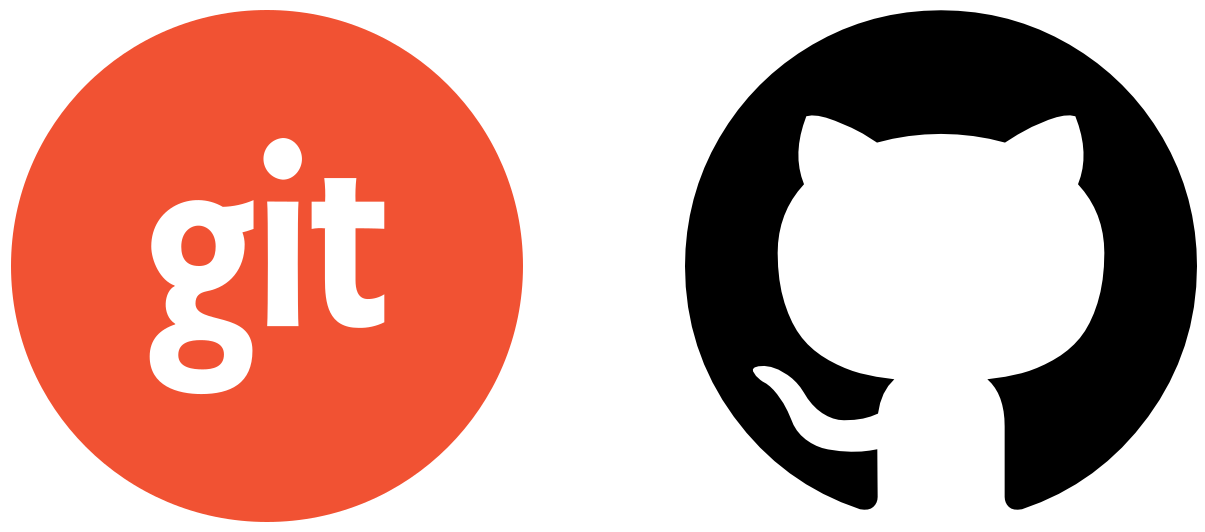
\includegraphics[width=4.16667in,height=\textheight]{unidades/unidad0/../../images/git_and_github.png}

}

\caption{Git and Github}

\end{figure}%

\section{¿Qué es Git y GitHub? 🕹️}\label{quuxe9-es-git-y-github}

\begin{itemize}
\item
  Git y GitHub son herramientas ampliamente utilizadas en el desarrollo
  de software para el control de versiones y la colaboración en
  proyectos.
\item
  Git es un sistema de control de versiones distribuido que permite
  realizar un seguimiento de los cambios en el código fuente durante el
  desarrollo de software. Fue creado por Linus Torvalds en 2005 y se
  utiliza mediante la línea de comandos o a través de interfaces
  gráficas de usuario.
\item
  GitHub, por otro lado, es una plataforma de alojamiento de
  repositorios Git en la nube. Proporciona un entorno colaborativo donde
  los desarrolladores pueden compartir y trabajar en proyectos de
  software de forma conjunta. Además, ofrece características adicionales
  como seguimiento de problemas, solicitudes de extracción y despliegue
  continuo.
\end{itemize}

En este tutorial, aprenderás los conceptos básicos de Git y GitHub, así
como su uso en un proyecto de software real.

\section{¿Quiénes utilizan Git? 🌍}\label{quiuxe9nes-utilizan-git}

\begin{figure}[H]

{\centering 
\includegraphics[width=6.25in,height=\textheight]{unidades/unidad0/../../images/git-logo-sticker.png}

}

\caption{Git}

\end{figure}%

Es ampliamente utilizado por desarrolladores de software en todo el
mundo, desde estudiantes hasta grandes empresas tecnológicas. Es una
herramienta fundamental para el desarrollo colaborativo y la gestión de
proyectos de software.

\section{¿Cómo se utiliza Git? 💻}\label{cuxf3mo-se-utiliza-git}

\begin{figure}[H]

{\centering 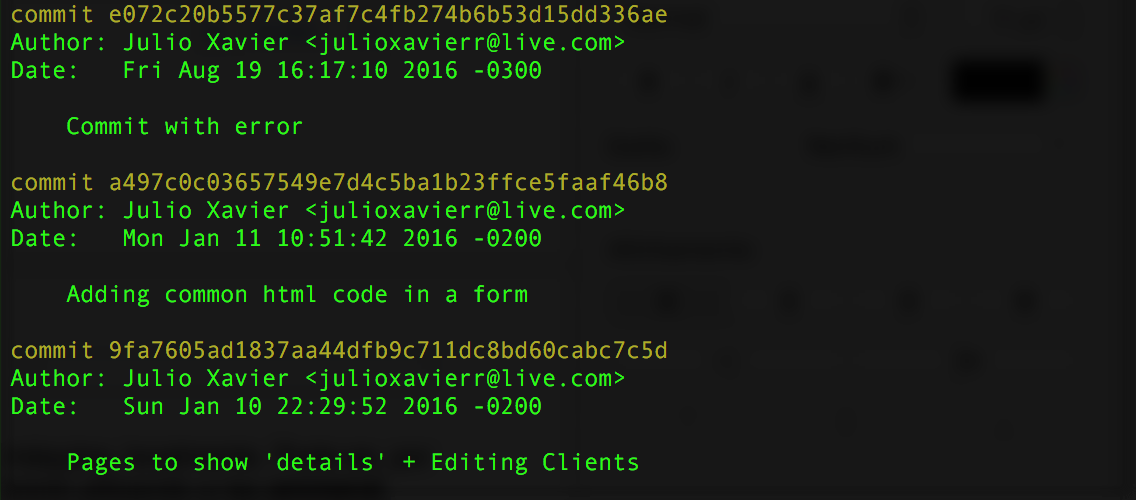
\includegraphics[width=6.25in,height=\textheight]{unidades/unidad0/../../images/git_terminal.png}

}

\caption{Git en Terminal}

\end{figure}%

Se utiliza mediante la \textbf{línea de comandos} o a través de
\textbf{interfaces gráficas} de usuario. Proporciona comandos para
realizar operaciones como:

\begin{enumerate}
\def\labelenumi{\arabic{enumi}.}
\tightlist
\item
  Inicializar un repositorio,
\item
  Realizar cambios,
\item
  Revisar historial,
\item
  Fusionar ramas,
\item
  Entre otros.
\end{enumerate}

\section{¿Para qué sirve Git? 📝}\label{para-quuxe9-sirve-git}

\begin{figure}[H]

{\centering 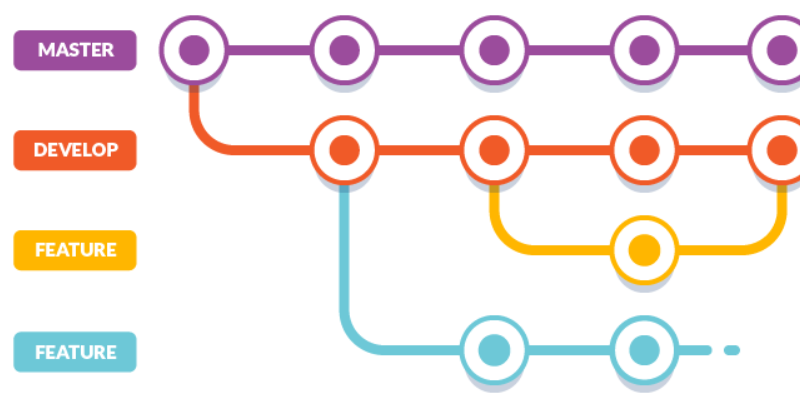
\includegraphics[width=6.25in,height=\textheight]{unidades/unidad0/../../images/seguimiento_cambios_git.png}

}

\caption{Seguimiento de Cambios con Git}

\end{figure}%

Sirve para realizar un seguimiento de los cambios en el código fuente,
coordinar el trabajo entre varios desarrolladores, revertir cambios no
deseados y mantener un historial completo de todas las modificaciones
realizadas en un proyecto.

\section{¿Por qué utilizar Git? 🤔}\label{por-quuxe9-utilizar-git}

\begin{figure}[H]

{\centering 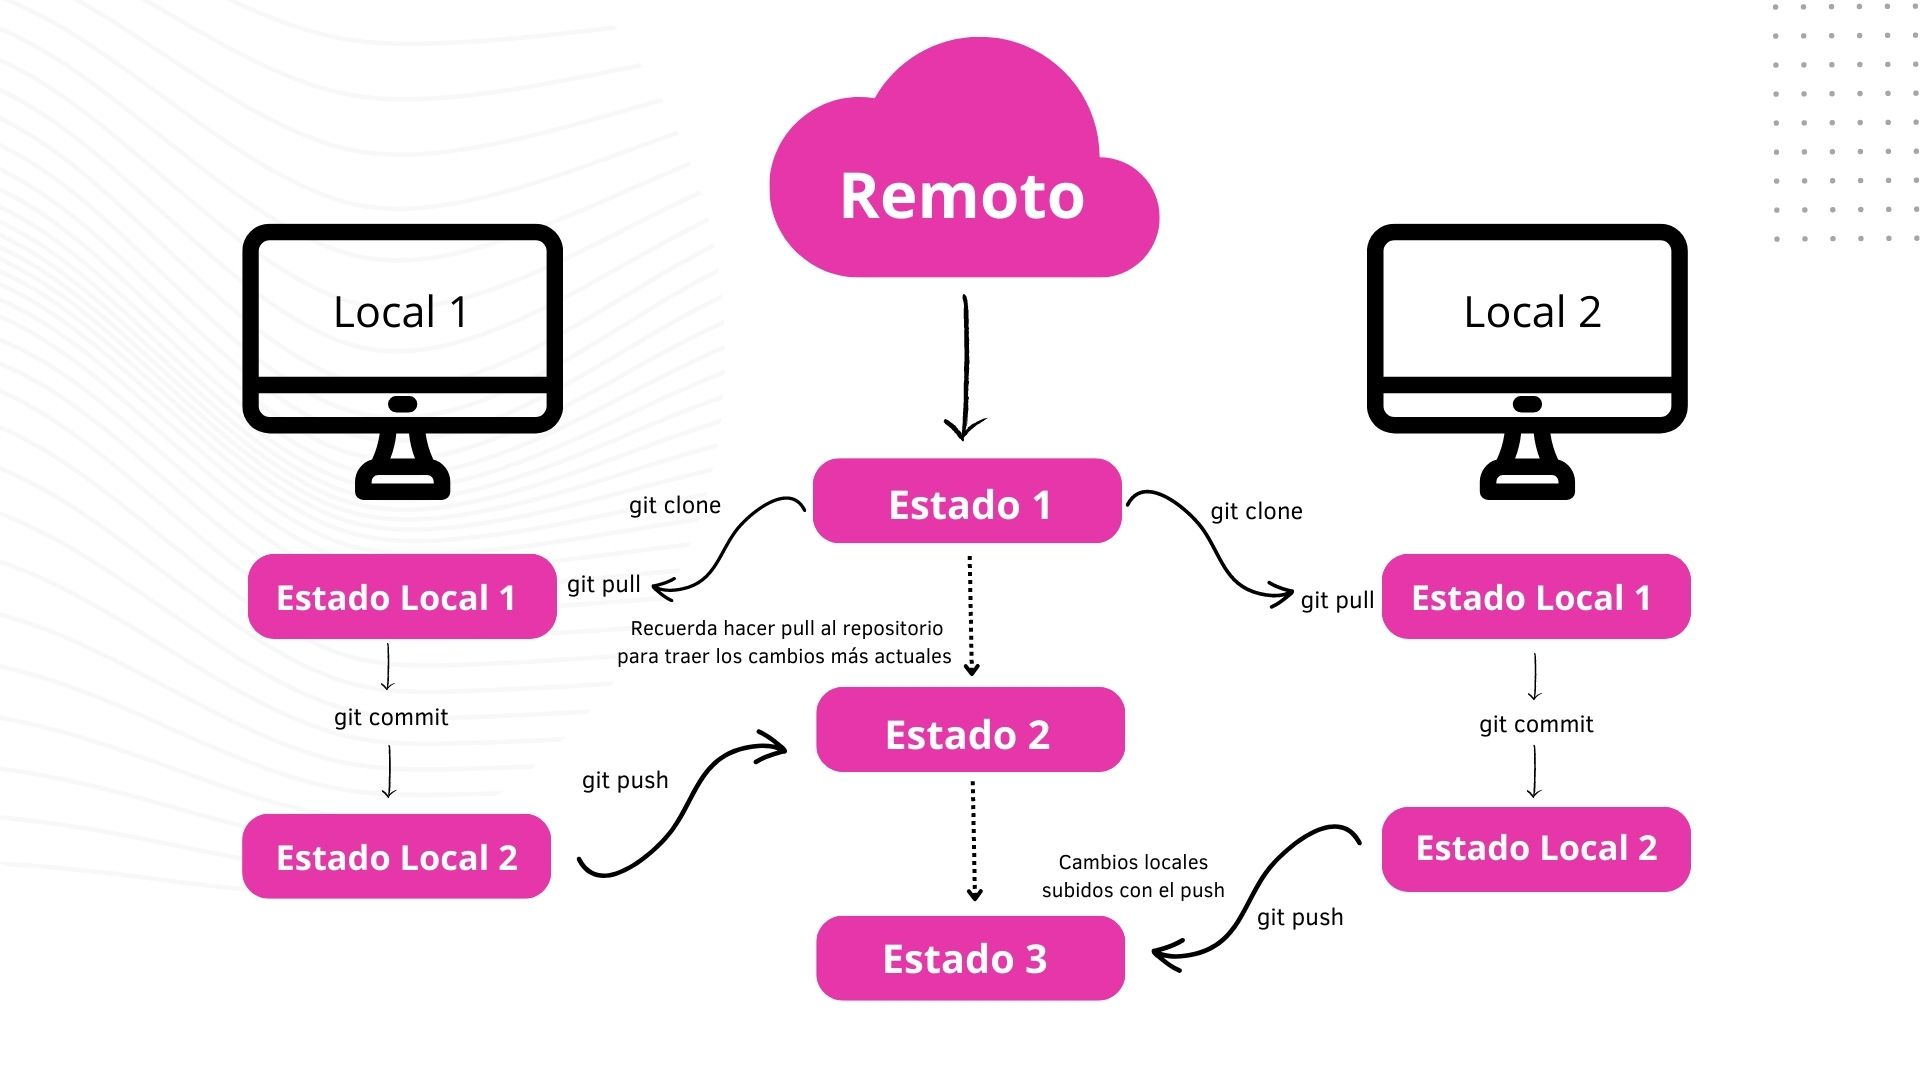
\includegraphics[width=6.25in,height=\textheight]{unidades/unidad0/../../images/ventajas_git.jpg}

}

\caption{Ventajas de Git}

\end{figure}%

Ofrece varias ventajas, como:

\begin{itemize}
\tightlist
\item
  La capacidad de trabajar de forma distribuida
\item
  La gestión eficiente de ramas para desarrollar nuevas funcionalidades
\item
  Corregir errores sin afectar la rama principal
\item
  La posibilidad de colaborar de forma efectiva con otros
  desarrolladores.
\end{itemize}

\section{¿Dónde puedo utilizar Git?
🌐}\label{duxf3nde-puedo-utilizar-git}

\begin{figure}[H]

{\centering 
\includegraphics[width=6.25in,height=\textheight]{unidades/unidad0/../../images/sistemas_operativos_git.png}

}

\caption{Git en Diferentes Sistemas Operativos}

\end{figure}%

Puede ser utilizado en cualquier sistema operativo, incluyendo Windows,
macOS y Linux. Además, es compatible con una amplia variedad de
plataformas de alojamiento de repositorios, siendo GitHub una de las más
populares.

\section{Pasos Básicos 📝}\label{pasos-buxe1sicos}

\begin{tcolorbox}[enhanced jigsaw, bottomrule=.15mm, rightrule=.15mm, colframe=quarto-callout-tip-color-frame, arc=.35mm, breakable, colbacktitle=quarto-callout-tip-color!10!white, toptitle=1mm, colback=white, opacitybacktitle=0.6, opacityback=0, bottomtitle=1mm, toprule=.15mm, titlerule=0mm, left=2mm, coltitle=black, leftrule=.75mm, title=\textcolor{quarto-callout-tip-color}{\faLightbulb}\hspace{0.5em}{Tip}]

Es recomendable tomar en cuenta una herramienta para la edición de
código, como Visual Studio Code, Sublime Text o Atom, para trabajar con
Git y GitHub de manera eficiente.

\end{tcolorbox}

\section{Instalación de Visual Studio Code
📥}\label{instalaciuxf3n-de-visual-studio-code}

\begin{figure}[H]

{\centering 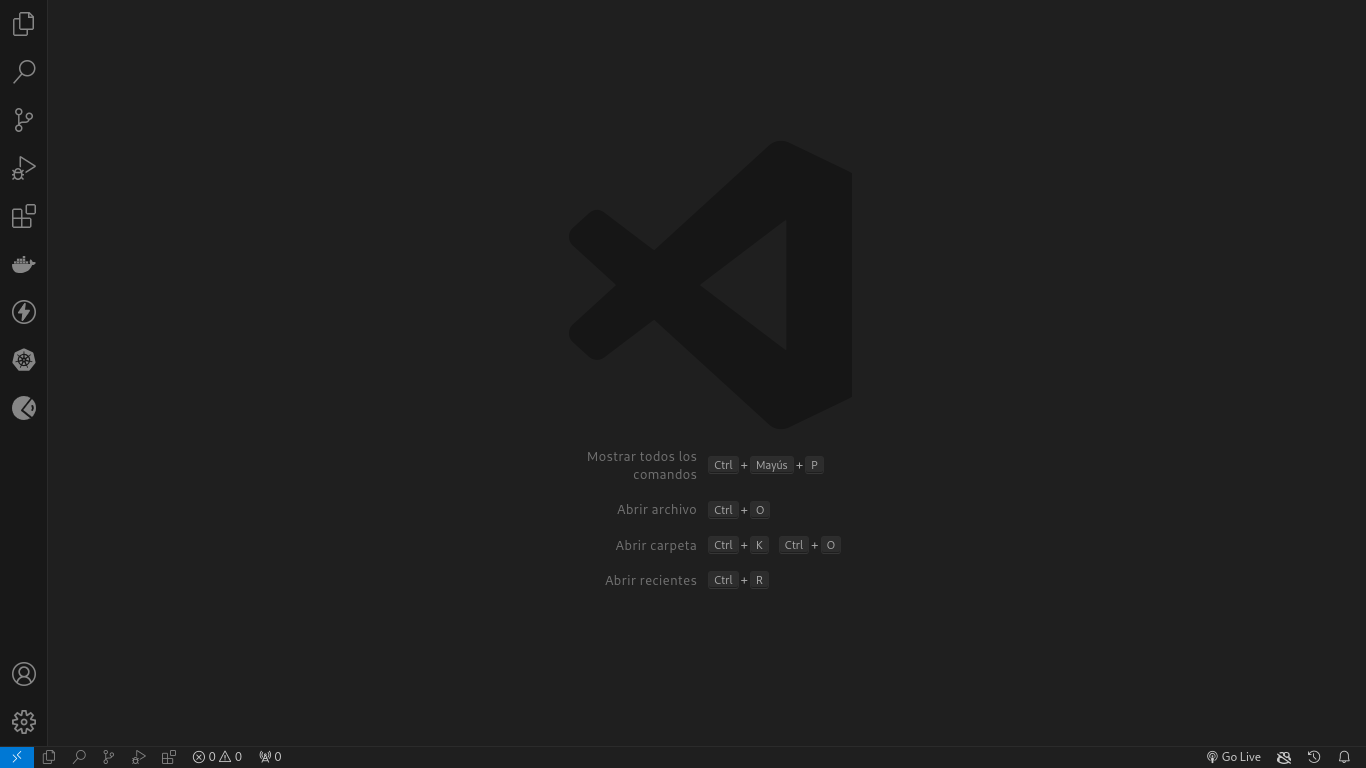
\includegraphics[width=6.25in,height=\textheight]{unidades/unidad0/../../images/vscode.png}

}

\caption{Visual Studio Code}

\end{figure}%

Si aún no tienes Visual Studio Code instalado, puedes descargarlo desde
\url{https://code.visualstudio.com/download}. Es una herramienta
gratuita y de código abierto que proporciona una interfaz amigable para
trabajar con Git y GitHub.

A continuación se presentan los pasos básicos para utilizar Git y GitHub
en un proyecto de software.

\subsection{Descarga e Instalación de Git
📥}\label{descarga-e-instalaciuxf3n-de-git}

\begin{figure}[H]

{\centering 
\includegraphics[width=6.25in,height=\textheight]{unidades/unidad0/../../images/website-git.png}

}

\caption{Git}

\end{figure}%

\begin{enumerate}
\def\labelenumi{\arabic{enumi}.}
\tightlist
\item
  Visita el sitio web oficial de Git en
  \url{https://git-scm.com/downloads}.
\item
  Descarga el instalador adecuado para tu sistema operativo y sigue las
  instrucciones de instalación.
\end{enumerate}

\subsection{Configuración 🛠️}\label{configuraciuxf3n}

\begin{figure}[H]

{\centering 
\includegraphics[width=6.25in,height=\textheight]{unidades/unidad0/../../images/git_config.png}

}

\caption{Configuración de Git}

\end{figure}%

Una vez instalado Git, es necesario configurar tu nombre de usuario y
dirección de correo electrónico. Esto se puede hacer mediante los
siguientes comandos:

\begin{Shaded}
\begin{Highlighting}[]
\FunctionTok{git}\NormalTok{ config }\AttributeTok{{-}{-}global}\NormalTok{ user.name }\StringTok{"Tu Nombre"}
\FunctionTok{git}\NormalTok{ config }\AttributeTok{{-}{-}global}\NormalTok{ user.email }\StringTok{"tu@email.com"}
\end{Highlighting}
\end{Shaded}

\subsection{Creación de un Repositorio ``helloWorld'' en Python
🐍}\label{creaciuxf3n-de-un-repositorio-helloworld-en-python}

\begin{itemize}
\tightlist
\item
  Crea una nueva carpeta para tu proyecto y ábrela en Visual Studio
  Code.
\item
  Crea un archivo Python llamado \textbf{hello\_world.py} y escribe el
  siguiente código:
\end{itemize}

\begin{Shaded}
\begin{Highlighting}[]
\KeywordTok{def}\NormalTok{ welcome\_message():}
\NormalTok{    name }\OperatorTok{=} \BuiltInTok{input}\NormalTok{(}\StringTok{"Ingrese su nombre: "}\NormalTok{)}
    \BuiltInTok{print}\NormalTok{(}\StringTok{"Bienvenio,"}\NormalTok{, name, }\StringTok{"al curso de Django y React!"}\NormalTok{)}

\ControlFlowTok{if} \VariableTok{\_\_name\_\_} \OperatorTok{==} \StringTok{"\_\_main\_\_"}\NormalTok{:}
\NormalTok{    welcome\_message()}
\end{Highlighting}
\end{Shaded}

\begin{itemize}
\tightlist
\item
  Guarda el archivo y abre una terminal en Visual Studio Code.
\item
  Inicializa un repositorio Git en la carpeta de tu proyecto con el
  siguiente comando:
\end{itemize}

\begin{Shaded}
\begin{Highlighting}[]
\FunctionTok{git}\NormalTok{ init}
\end{Highlighting}
\end{Shaded}

\begin{itemize}
\tightlist
\item
  Añade el archivo al área de preparación con:
\end{itemize}

\begin{Shaded}
\begin{Highlighting}[]
\FunctionTok{git}\NormalTok{ add hello\_world.py}
\end{Highlighting}
\end{Shaded}

\begin{itemize}
\tightlist
\item
  Realiza un commit de los cambios con un mensaje descriptivo:
\end{itemize}

\begin{Shaded}
\begin{Highlighting}[]
\FunctionTok{git}\NormalTok{ commit }\AttributeTok{{-}m} \StringTok{"Añadir archivo hello\_world.py"}
\end{Highlighting}
\end{Shaded}

\subsection{Comandos Básicos de Git
📝}\label{comandos-buxe1sicos-de-git}

\begin{itemize}
\tightlist
\item
  \textbf{git init:} Inicializa un nuevo repositorio Git.
\item
  \textbf{git add :} Añade un archivo al área de preparación.
\item
  \textbf{git commit -m ``''}: Realiza un commit de los cambios con un
  mensaje descriptivo.
\item
  \textbf{git push:} Sube los cambios al repositorio remoto.
\item
  \textbf{git pull:} Descarga cambios del repositorio remoto.
\item
  \textbf{git branch:} Lista las ramas disponibles.
\item
  \textbf{git checkout :} Cambia a una rama específica.
\item
  \textbf{git merge :} Fusiona una rama con la rama actual.
\item
  \textbf{git reset :} Descarta los cambios en un archivo.
\item
  \textbf{git diff:} Muestra las diferencias entre versiones.
\end{itemize}

\subsection{Estados en Git 📊}\label{estados-en-git}

\begin{itemize}
\tightlist
\item
  \textbf{Local:} Representa los cambios que realizas en tu repositorio
  local antes de hacer un commit. Estos cambios están únicamente en tu
  máquina.
\item
  \textbf{Staging:} Indica los cambios que has añadido al área de
  preparación con el comando \texttt{git\ add}. Estos cambios están
  listos para ser confirmados en el próximo commit.
\item
  \textbf{Commit:} Son los cambios que has confirmado en tu repositorio
  local con el comando \texttt{git\ commit}. Estos cambios se han
  guardado de manera permanente en tu repositorio local.
\item
  \textbf{Server:} Son los cambios que has subido al repositorio remoto
  con el comando \texttt{git\ push}. Estos cambios están disponibles
  para otros colaboradores del proyecto.
\end{itemize}

\begin{center}\rule{0.5\linewidth}{0.5pt}\end{center}

\chapter{Tutorial: Moviendo Cambios entre Estados en Git
📝}\label{tutorial-moviendo-cambios-entre-estados-en-git}

\section{Introducción}\label{introducciuxf3n}

En este tutorial, aprenderemos a utilizar Git para gestionar cambios en
nuestro proyecto y moverlos entre diferentes estados. Utilizaremos un
ejemplo práctico para comprender mejor estos conceptos.

\begin{Shaded}
\begin{Highlighting}[]
\KeywordTok{def}\NormalTok{ welcome\_message():}
\NormalTok{    name }\OperatorTok{=} \BuiltInTok{input}\NormalTok{(}\StringTok{"Ingrese su nombre: "}\NormalTok{)}
    \BuiltInTok{print}\NormalTok{(}\StringTok{"Bienvenio,"}\NormalTok{, name, }\StringTok{"al curso de Django y React!"}\NormalTok{)}

\ControlFlowTok{if} \VariableTok{\_\_name\_\_} \OperatorTok{==} \StringTok{"\_\_main\_\_"}\NormalTok{:}
\NormalTok{    welcome\_message()}
\end{Highlighting}
\end{Shaded}

\section{Sección 1: Modificar Archivos en el
Repositorio}\label{secciuxf3n-1-modificar-archivos-en-el-repositorio}

En esta sección, aprenderemos cómo realizar cambios en nuestros archivos
y reflejarlos en Git.

\section{Mover Cambios de Local a
Staging:}\label{mover-cambios-de-local-a-staging}

\begin{enumerate}
\def\labelenumi{\arabic{enumi}.}
\tightlist
\item
  Abre el archivo \textbf{hello\_world.py} en Visual Studio Code.
\item
  Modifica el mensaje de bienvenida a ``Bienvenido'' en lugar de
  ``Bienvenio''.
\item
  Guarda los cambios y abre una terminal en Visual Studio Code.
\end{enumerate}

Hemos corregido un error en nuestro archivo y queremos reflejarlo en
Git.

\begin{Shaded}
\begin{Highlighting}[]
\ExtensionTok{def}\NormalTok{ welcome\_message}\ErrorTok{(}\KeywordTok{)}\BuiltInTok{:}
    \ExtensionTok{name}\NormalTok{ = input}\ErrorTok{(}\StringTok{"Ingrese su nombre: "}\KeywordTok{)}
    \ExtensionTok{print}\ErrorTok{(}\StringTok{"Bienvenido,"}\ExtensionTok{,}\NormalTok{ name, }\StringTok{"al curso de Django y React!"}\KeywordTok{)}

\ControlFlowTok{if} \ExtensionTok{\_\_name\_\_}\NormalTok{ == }\StringTok{"\_\_main\_\_"}\NormalTok{:}
    \FunctionTok{welcome\_message()}
\end{Highlighting}
\end{Shaded}

\section{Agregar Cambios de Local a
Staging:}\label{agregar-cambios-de-local-a-staging}

\begin{Shaded}
\begin{Highlighting}[]
\FunctionTok{git}\NormalTok{ add hello\_world.py}
\end{Highlighting}
\end{Shaded}

Hemos añadido los cambios al área de preparación y están listos para ser
confirmados en el próximo commit.

\section{Sección 2: Confirmar Cambios en un
Commit}\label{secciuxf3n-2-confirmar-cambios-en-un-commit}

En esta sección, aprenderemos cómo confirmar los cambios en un commit y
guardarlos de manera permanente en nuestro repositorio.

\section{Mover Cambios de Staging a
Commit:}\label{mover-cambios-de-staging-a-commit}

\begin{Shaded}
\begin{Highlighting}[]
\FunctionTok{git}\NormalTok{ commit }\AttributeTok{{-}m} \StringTok{"Corregir mensaje de bienvenida"}
\end{Highlighting}
\end{Shaded}

Hemos confirmado los cambios en un commit con un mensaje descriptivo.

\section{Sección 3: Creación y Fusión de
Ramas}\label{secciuxf3n-3-creaciuxf3n-y-fusiuxf3n-de-ramas}

En esta sección, aprenderemos cómo crear y fusionar ramas en Git para
desarrollar nuevas funcionalidades de forma aislada.

\section{Crear una Nueva Rama:}\label{crear-una-nueva-rama}

\begin{Shaded}
\begin{Highlighting}[]
\FunctionTok{git}\NormalTok{ branch feature}
\end{Highlighting}
\end{Shaded}

Hemos creado una nueva rama llamada ``feature'' para desarrollar una
nueva funcionalidad.

\section{Implementar Funcionalidades en la
Rama:}\label{implementar-funcionalidades-en-la-rama}

\begin{enumerate}
\def\labelenumi{\arabic{enumi}.}
\tightlist
\item
  Abre el archivo \textbf{hello\_world.py} en Visual Studio Code.
\item
  Añade una nueva función para mostrar un mensaje de despedida.
\item
  Guarda los cambios y abre una terminal en Visual Studio Code.
\item
  Añade los cambios al área de preparación y confírmalos en un commit.
\item
  Cambia a la rama principal con \texttt{git\ checkout\ main}.
\end{enumerate}

\section{Fusionar Ramas con la Rama
Principal:}\label{fusionar-ramas-con-la-rama-principal}

\begin{Shaded}
\begin{Highlighting}[]
\FunctionTok{git}\NormalTok{ merge feature}
\end{Highlighting}
\end{Shaded}

Hemos fusionado la rama ``feature'' con la rama principal y añadido la
nueva funcionalidad al proyecto.

\section{Sección 4: Revertir Cambios en un
Archivo}\label{secciuxf3n-4-revertir-cambios-en-un-archivo}

En esta sección, aprenderemos cómo revertir cambios en un archivo y
deshacerlos en Git.

\section{Revertir Cambios en un
Archivo:}\label{revertir-cambios-en-un-archivo}

\begin{Shaded}
\begin{Highlighting}[]
\FunctionTok{git}\NormalTok{ reset hello\_world.py}
\end{Highlighting}
\end{Shaded}

Hemos revertido los cambios en el archivo \textbf{hello\_world.py} y
deshecho las modificaciones realizadas.

\section{Conclusión}\label{conclusiuxf3n}

En este tutorial, hemos aprendido a gestionar cambios en nuestro
proyecto y moverlos entre diferentes estados en Git. Estos conceptos son
fundamentales para trabajar de forma eficiente en proyectos de software
y colaborar con otros desarrolladores.

\chapter{Asignación}\label{asignaciuxf3n}

\href{https://classroom.github.com/a/o-qydr2W}{Hello World!}

Este proyecto de ejemplo está escrito en Python y se prueba con pytest.

\textbf{La Asignación}

Las pruebas están fallando en este momento porque el método no está
devolviendo la cadena correcta. Corrige el código del archivo
\textbf{hello.py} para que las pruebas sean exitosas, debe devolver la
cadena correcta \textbf{``Hello World!''}x

El comando de ejecución del test es:

\begin{Shaded}
\begin{Highlighting}[]
\ExtensionTok{pytest}\NormalTok{ test\_hello.py}
\end{Highlighting}
\end{Shaded}

¡Mucha suerte!

\chapter{GitHub Classroom 📒}\label{github-classroom}

\begin{figure}[H]

{\centering 
\includegraphics[width=1.04167in,height=\textheight]{unidades/unidad0/../../images/github classroom.png}

}

\caption{Github Classroom}

\end{figure}%

GitHub Classroom es una herramienta poderosa que facilita la gestión de
tareas y asignaciones en GitHub, especialmente diseñada para entornos
educativos.

\section{¿Qué es GitHub Classroom? 🤔}\label{quuxe9-es-github-classroom}

\begin{figure}[H]

{\centering 
\includegraphics[width=4.16667in,height=\textheight]{unidades/unidad0/../../images/github-classroom-ventana.jpg}

}

\caption{Github Classroom Windows}

\end{figure}%

GitHub Classroom es una extensión de GitHub que permite a los profesores
crear y gestionar asignaciones utilizando repositorios de GitHub.
Proporciona una forma organizada y eficiente de distribuir tareas a los
estudiantes, recopilar y revisar su trabajo, y proporcionar
retroalimentación.

\subsection{Funcionalidades Principales
⚙️}\label{funcionalidades-principales}

\textbf{Creación de Asignaciones:} Los profesores pueden crear tareas y
asignaciones directamente desde GitHub Classroom, proporcionando
instrucciones detalladas y estableciendo criterios de evaluación.

\textbf{Distribución Automatizada:} Una vez que se crea una asignación,
GitHub Classroom genera automáticamente repositorios privados para cada
estudiante o equipo, basándose en una plantilla predefinida.

\textbf{Seguimiento de Progreso:} Los profesores pueden realizar un
seguimiento del progreso de los estudiantes y revisar sus contribuciones
a través de solicitudes de extracción (pull requests) y comentarios en
el código.

\textbf{Revisión y Retroalimentación:} Los estudiantes envían sus
trabajos a través de solicitudes de extracción, lo que permite a los
profesores revisar y proporcionar retroalimentación específica sobre su
código.

\section{Ejemplo Práctico}\label{ejemplo-pruxe1ctico}

\subsection{Creación de una Asignación en GitHub Classroom
📒}\label{creaciuxf3n-de-una-asignaciuxf3n-en-github-classroom}

\textbf{Iniciar Sesión:} Ingresa a GitHub Classroom con tu cuenta de
GitHub y selecciona la opción para crear una nueva asignación.

\begin{center}
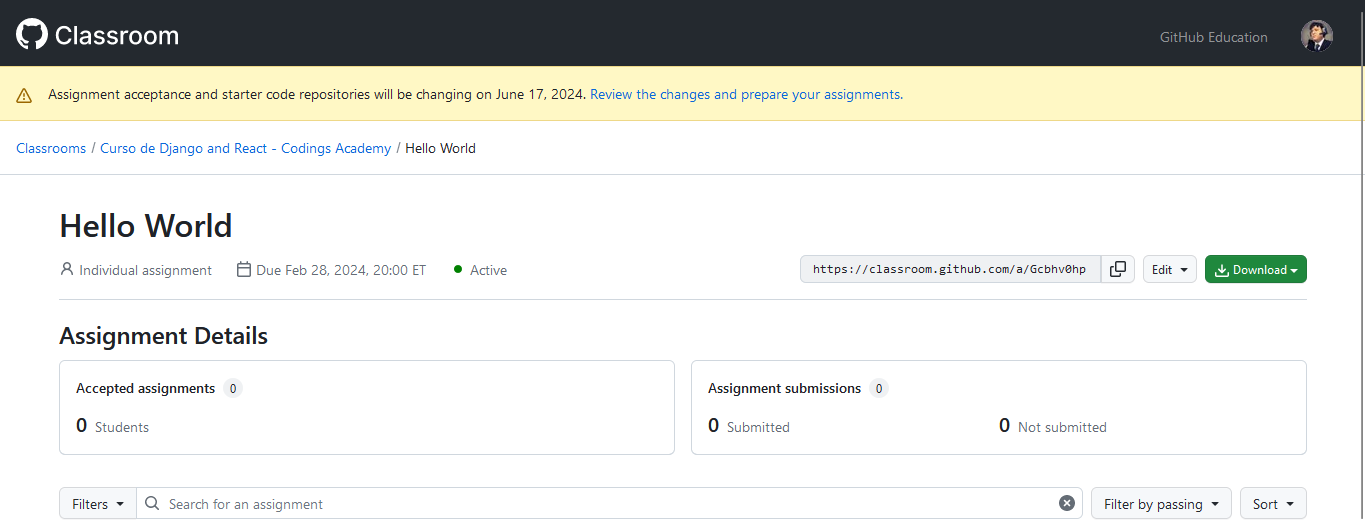
\includegraphics{unidades/unidad0/images/paste-2.png}
\end{center}

\textbf{Definir la Tarea:} Proporciona instrucciones claras y detalladas
sobre la tarea, incluyendo cualquier código base o recursos necesarios.
Establece los criterios de evaluación para guiar a los estudiantes.

\begin{center}
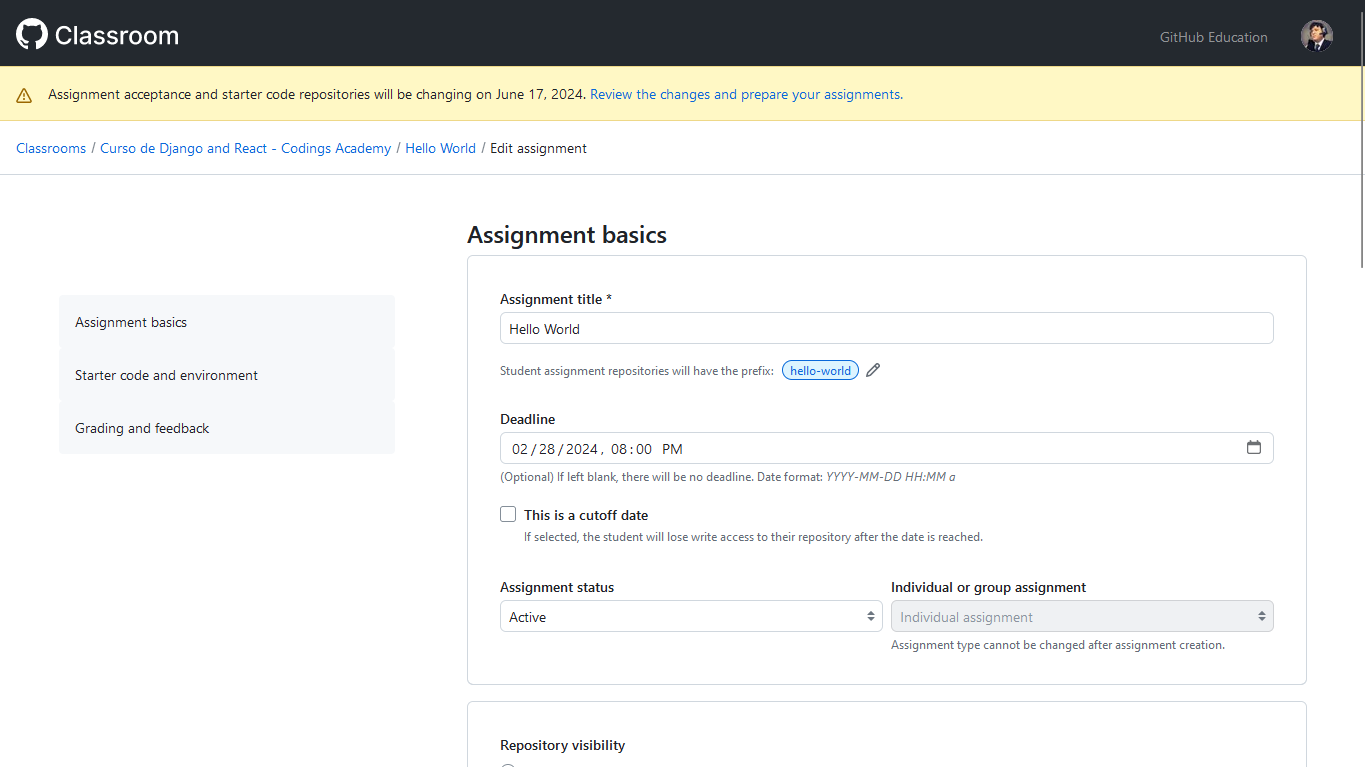
\includegraphics{unidades/unidad0/images/paste-1.png}
\end{center}

\textbf{Configurar la Plantilla:} Selecciona una plantilla de
repositorio existente o crea una nueva plantilla que servirá como base
para los repositorios de los estudiantes.

\begin{center}
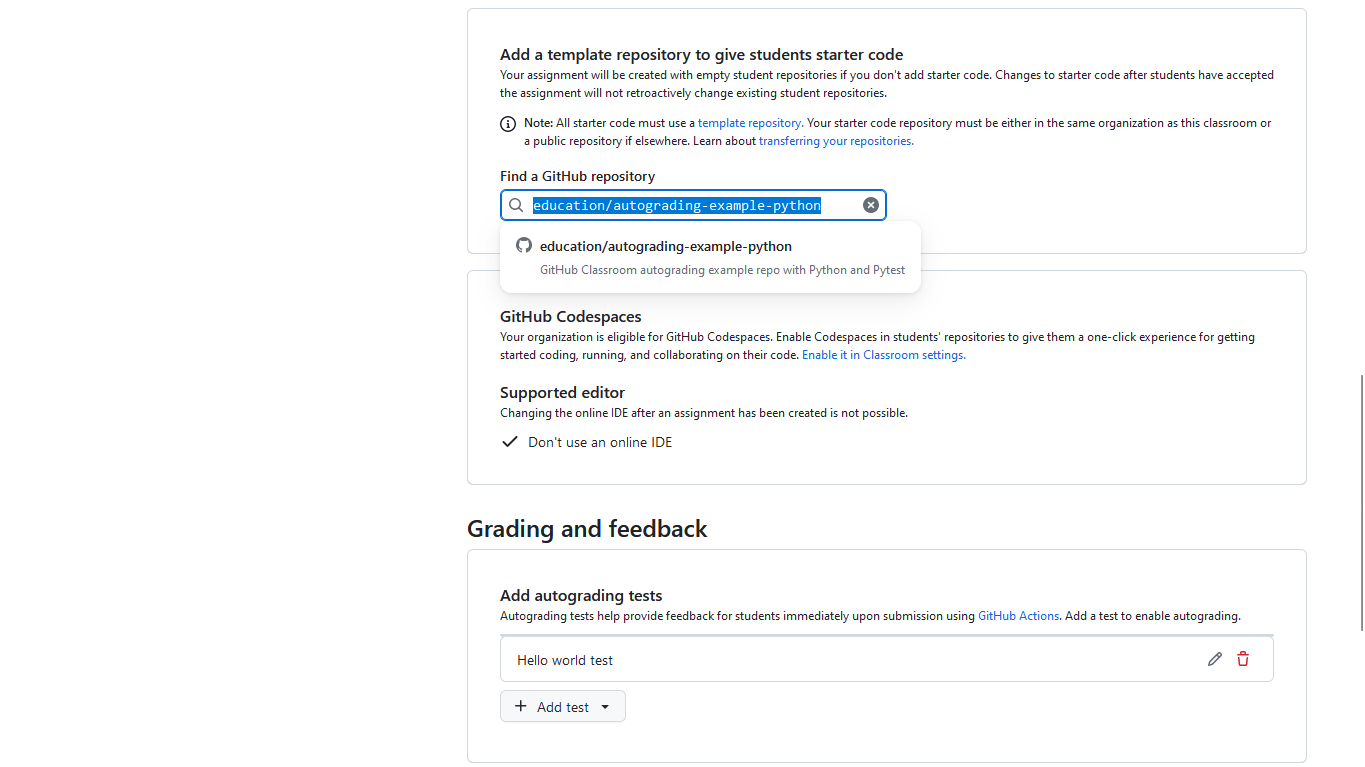
\includegraphics{unidades/unidad0/images/paste-3.png}
\end{center}

\textbf{Distribuir la Asignación:} Una vez configurada la asignación,
comparte el enlace generado con tus estudiantes para que puedan acceder
a sus repositorios privados.

\begin{center}
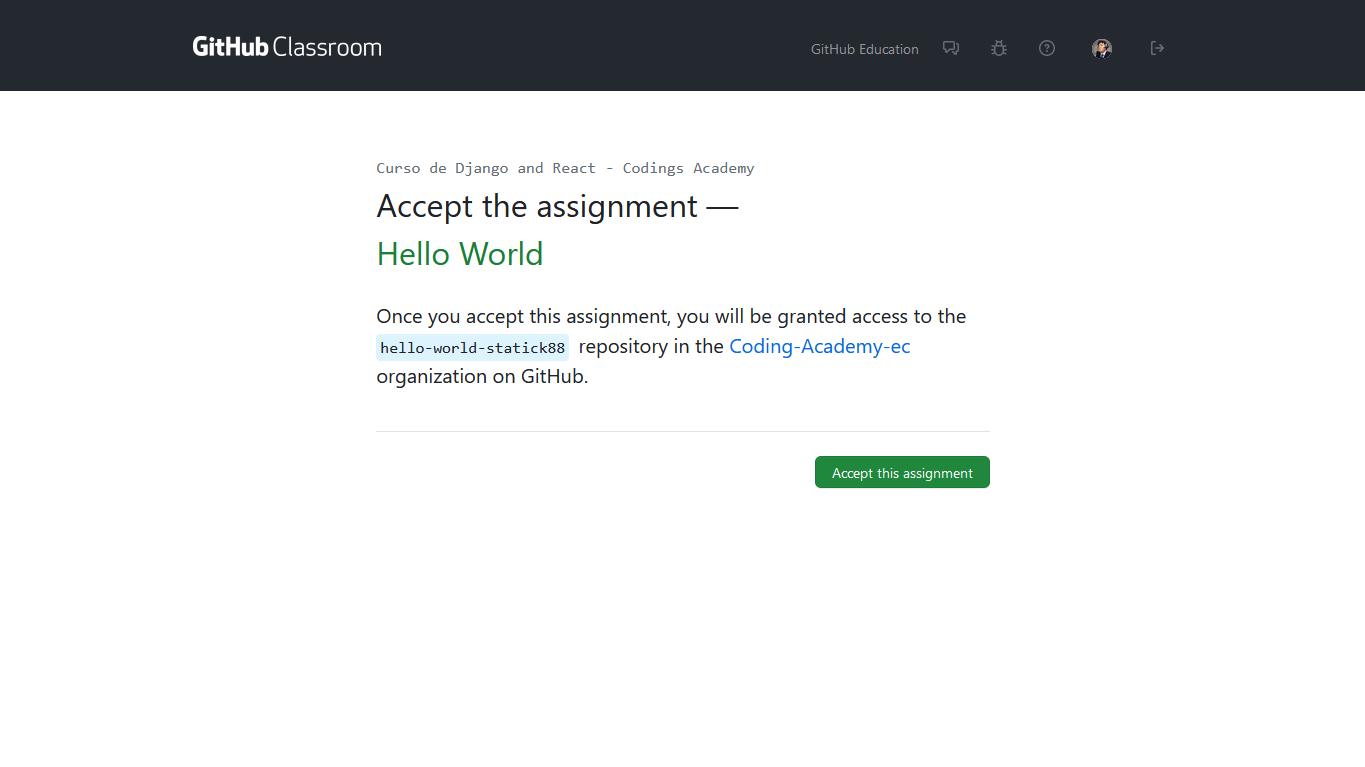
\includegraphics{unidades/unidad0/images/paste-4.png}
\end{center}

\section{Trabajo de los Estudiantes
🧑‍💻}\label{trabajo-de-los-estudiantes}

\textbf{Aceptar la Asignación:} Los estudiantes reciben el enlace de la
asignación y aceptan la tarea, lo que les permite crear un repositorio
privado basado en la plantilla proporcionada.

\begin{center}
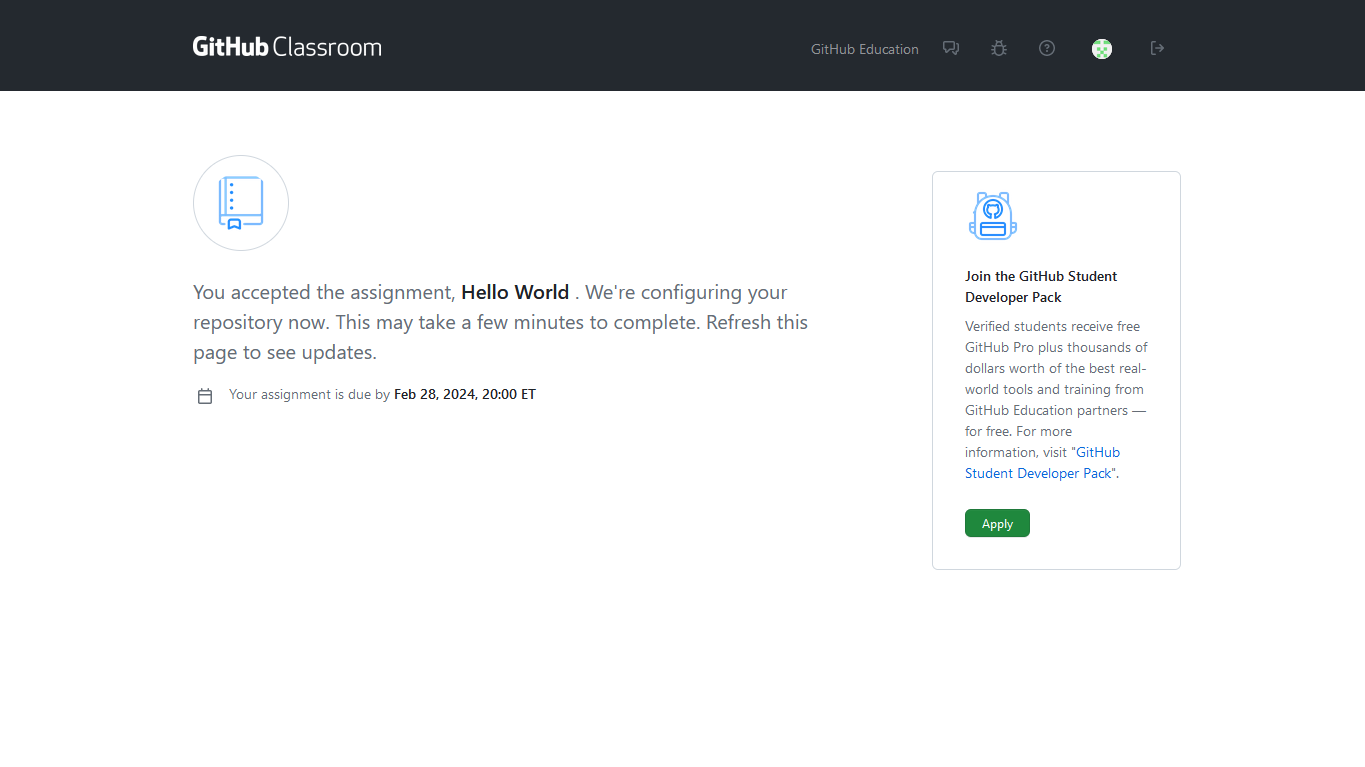
\includegraphics{unidades/unidad0/images/paste-6.png}
\end{center}

\textbf{Actualizar el Navegador:} Los estudiantes actualizan su
navegador para ver el nuevo repositorio creado en su cuenta de GitHub.

\begin{center}
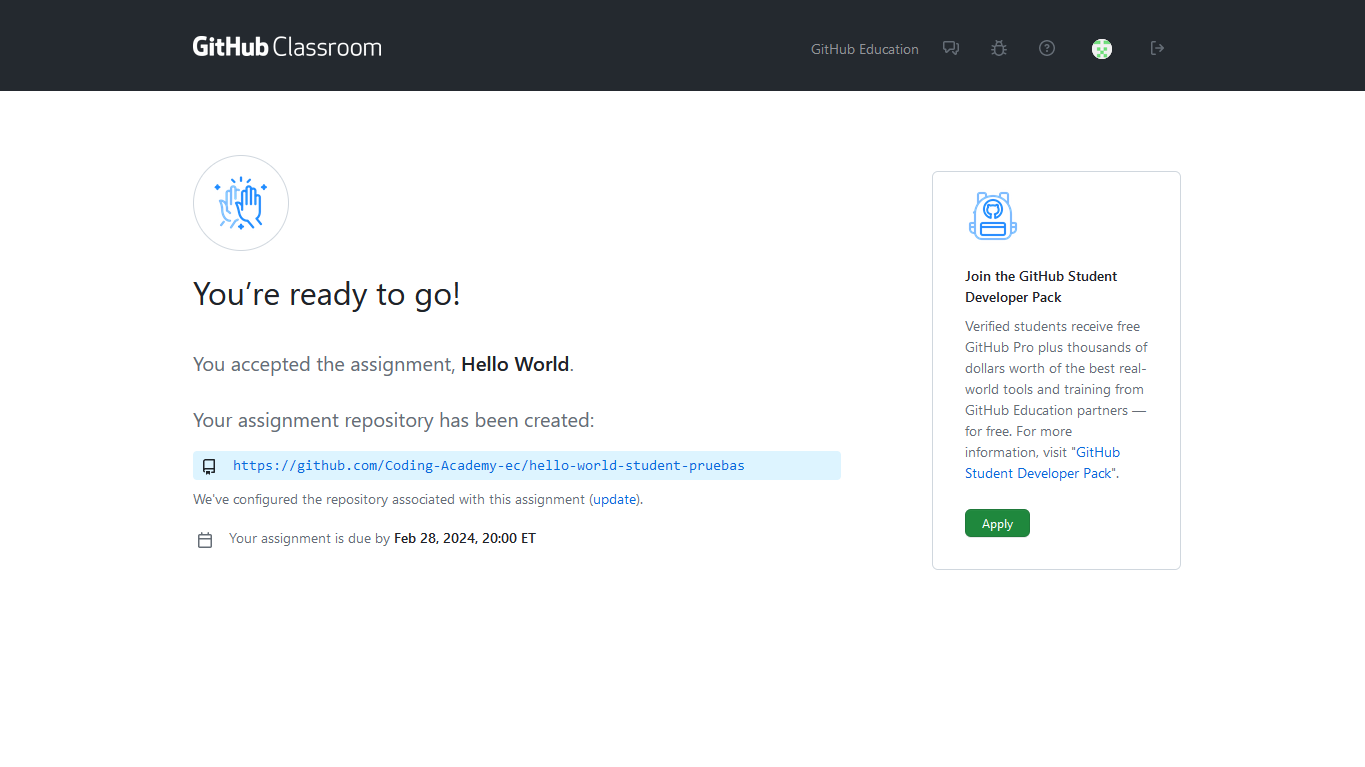
\includegraphics{unidades/unidad0/images/paste-8.png}
\end{center}

\textbf{Clonar el Repositorio:} Los estudiantes clonan el repositorio
asignado en su computadora local utilizando el enlace proporcionado.

\begin{center}
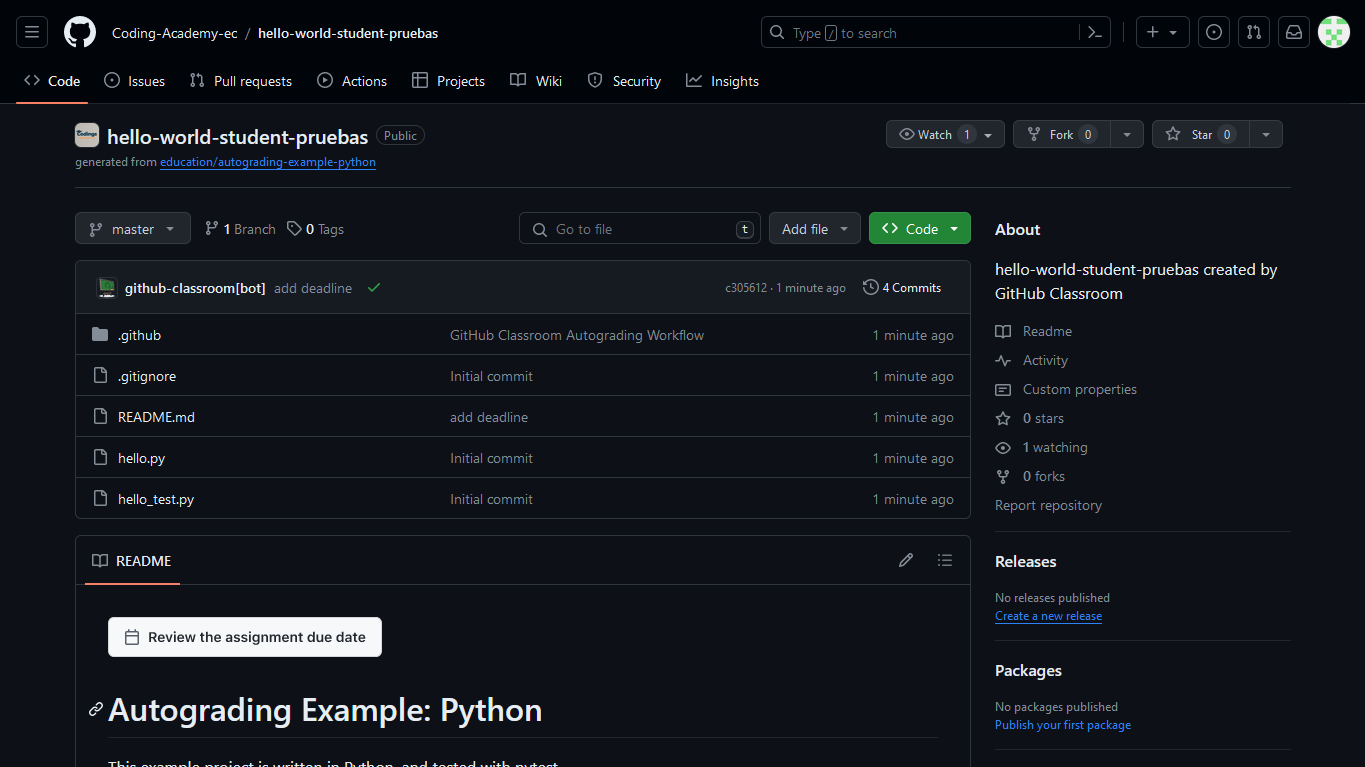
\includegraphics{unidades/unidad0/images/paste-9.png}
\end{center}

Utilizar el comando git clone: Aplique el comando git clone para clonar
el repositorio en su computadora local.

\begin{Shaded}
\begin{Highlighting}[]
\FunctionTok{git}\NormalTok{ clone }\OperatorTok{\textless{}}\NormalTok{enlace{-}del{-}repositorio}\OperatorTok{\textgreater{}}
\end{Highlighting}
\end{Shaded}

\begin{center}
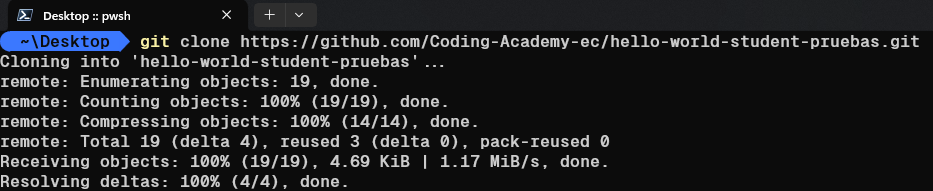
\includegraphics{unidades/unidad0/images/paste-10.png}
\end{center}

\textbf{Desarrollar la Tarea:} Los estudiantes trabajan en la tarea,
realizando los cambios necesarios y realizando commits de manera regular
para mantener un historial de su trabajo.

\begin{tcolorbox}[enhanced jigsaw, bottomrule=.15mm, rightrule=.15mm, colframe=quarto-callout-tip-color-frame, arc=.35mm, breakable, colbacktitle=quarto-callout-tip-color!10!white, toptitle=1mm, colback=white, opacitybacktitle=0.6, opacityback=0, bottomtitle=1mm, toprule=.15mm, titlerule=0mm, left=2mm, coltitle=black, leftrule=.75mm, title=\textcolor{quarto-callout-tip-color}{\faLightbulb}\hspace{0.5em}{Tip}]

Puedes probar el test incorporado con el comando \texttt{pytest} en la
terminal, para verificar que el código cumple con los requerimientos

\end{tcolorbox}

\begin{Shaded}
\begin{Highlighting}[]
\ExtensionTok{pytest}
\end{Highlighting}
\end{Shaded}

Una vez desarrollado el código de acuerdo a la asignación en local
deberían pasar el o los test

\begin{center}
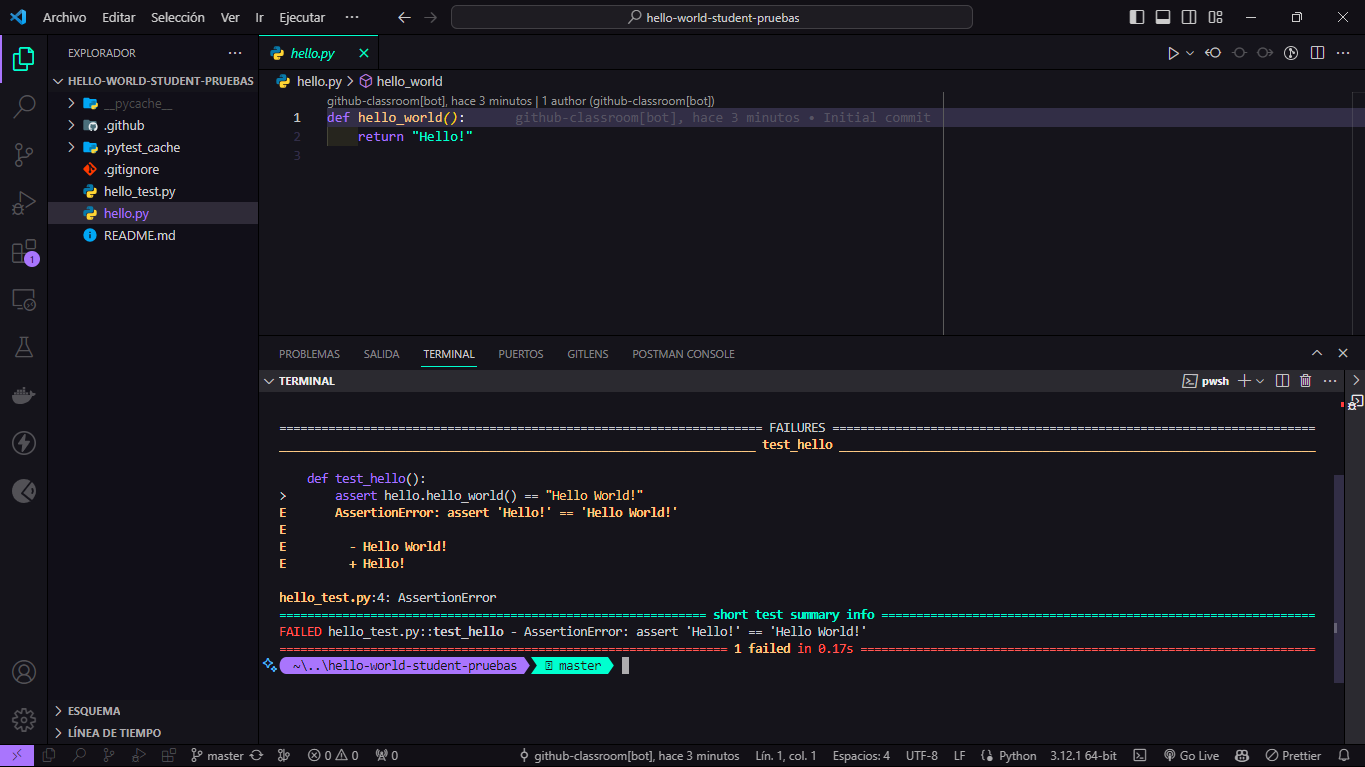
\includegraphics{unidades/unidad0/images/paste-11.png}
\end{center}

\textbf{Enviar la Solicitud de Extracción:} Una vez completada la tarea,
los estudiantes envían una solicitud de extracción desde su rama hacia
la rama principal del repositorio, solicitando la revisión del profesor.

\begin{center}
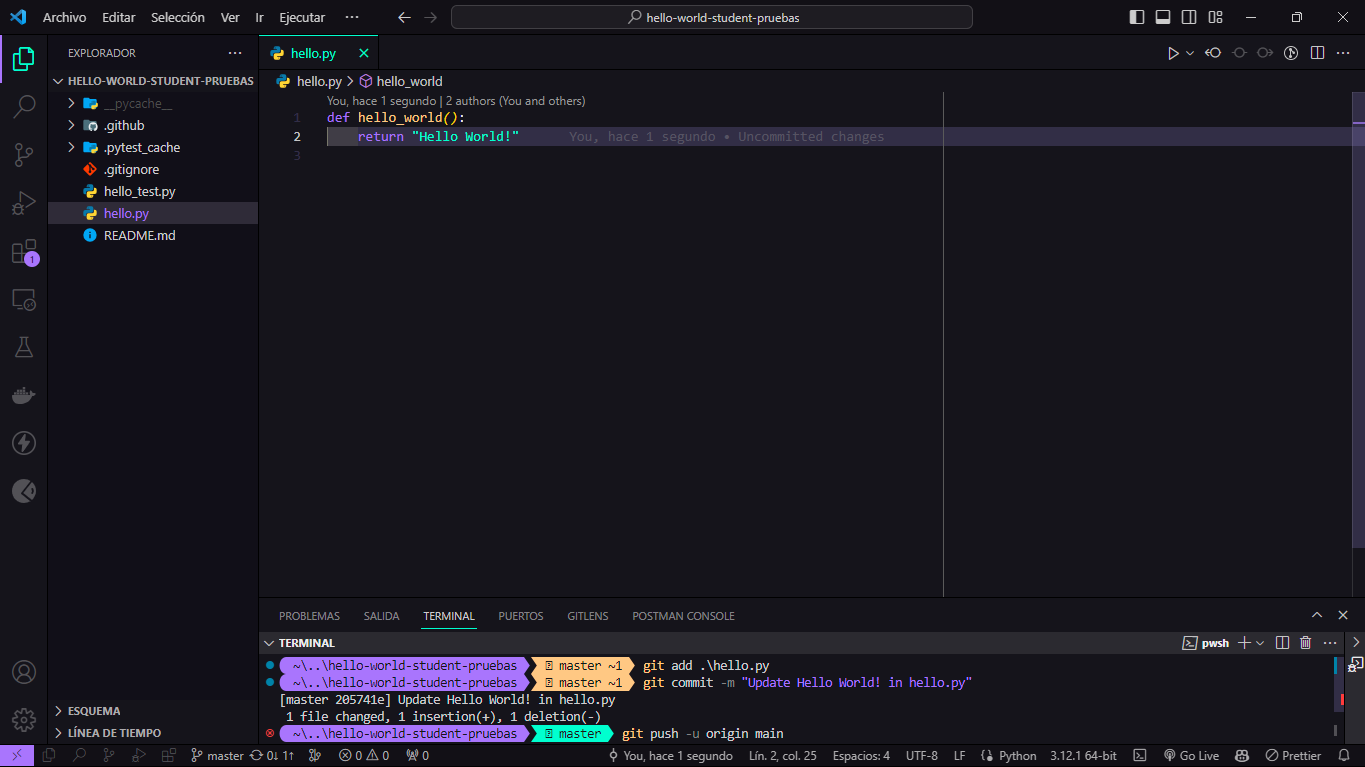
\includegraphics{unidades/unidad0/images/paste-12.png}
\end{center}

Una vez realizado el \texttt{push} se envía al respositorio principal y
se ejecutan los test en Github

\begin{tcolorbox}[enhanced jigsaw, bottomrule=.15mm, rightrule=.15mm, colframe=quarto-callout-tip-color-frame, arc=.35mm, breakable, colbacktitle=quarto-callout-tip-color!10!white, toptitle=1mm, colback=white, opacitybacktitle=0.6, opacityback=0, bottomtitle=1mm, toprule=.15mm, titlerule=0mm, left=2mm, coltitle=black, leftrule=.75mm, title=\textcolor{quarto-callout-tip-color}{\faLightbulb}\hspace{0.5em}{Tip}]

Se recomienda hacer las pruebas en local antes de enviar los cambios al
respositorio en Github

\end{tcolorbox}

\begin{center}
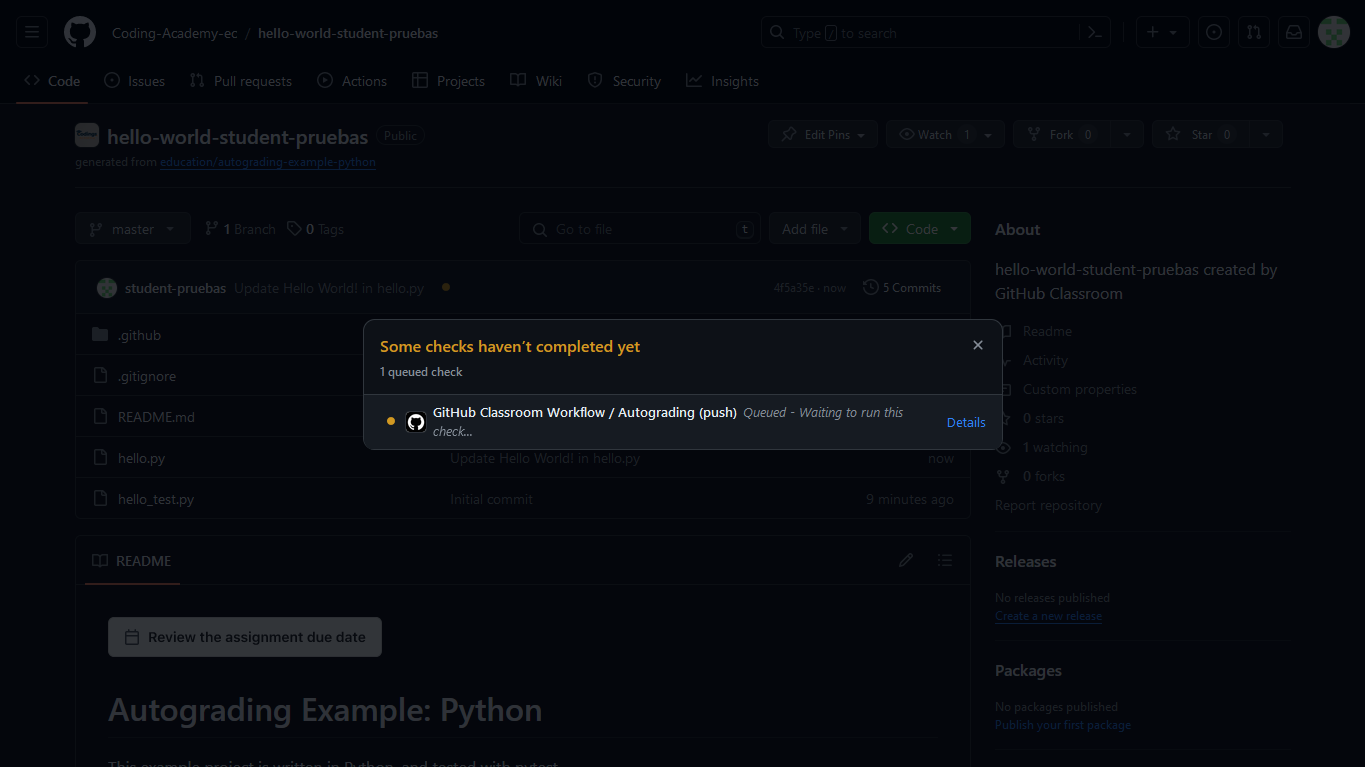
\includegraphics{unidades/unidad0/images/paste-13.png}
\end{center}

Este Action lo que hace es evaluar los cambios realizados

\begin{center}
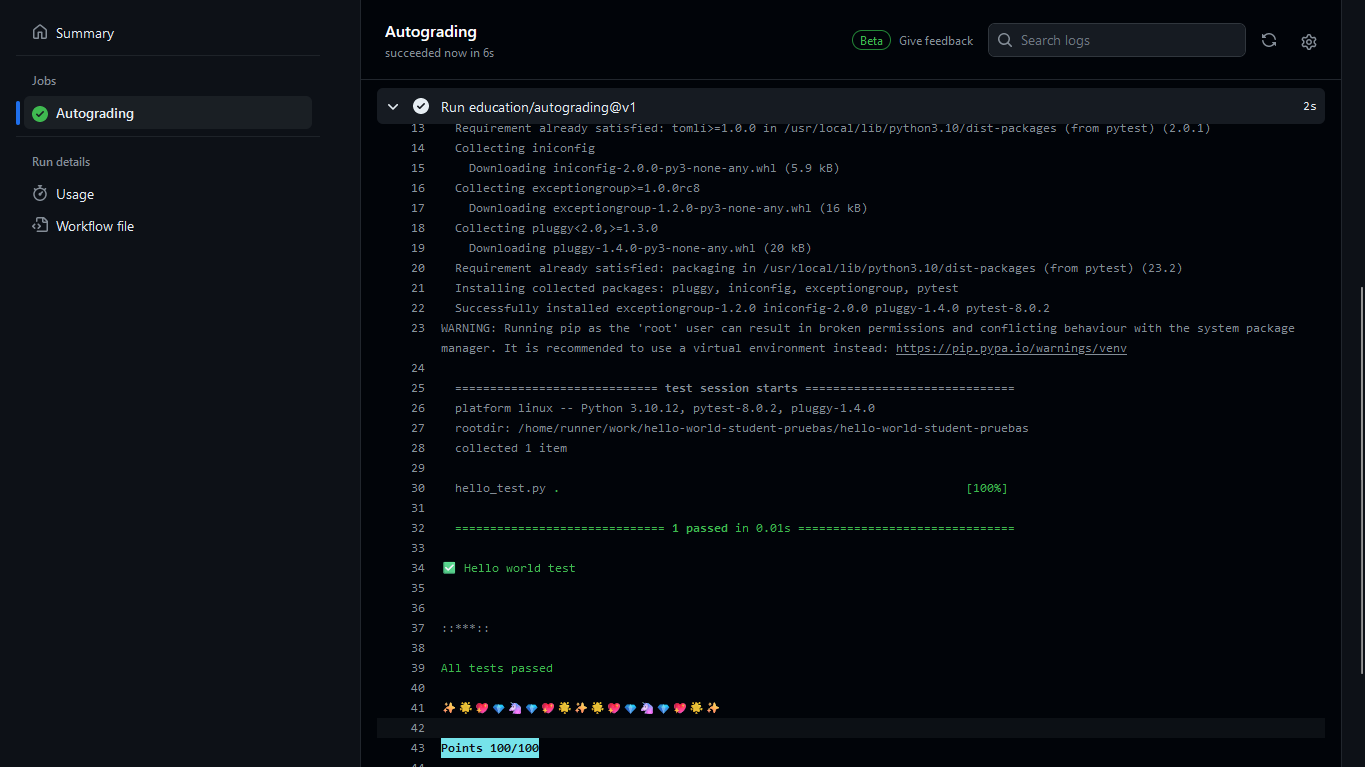
\includegraphics{unidades/unidad0/images/paste-14.png}
\end{center}

\begin{tcolorbox}[enhanced jigsaw, bottomrule=.15mm, rightrule=.15mm, colframe=quarto-callout-tip-color-frame, arc=.35mm, breakable, colbacktitle=quarto-callout-tip-color!10!white, toptitle=1mm, colback=white, opacitybacktitle=0.6, opacityback=0, bottomtitle=1mm, toprule=.15mm, titlerule=0mm, left=2mm, coltitle=black, leftrule=.75mm, title=\textcolor{quarto-callout-tip-color}{\faLightbulb}\hspace{0.5em}{Tip}]

Se recomienda hacer las pruebas en local antes de enviar los cambios al
respositorio en Github

\end{tcolorbox}

\textbf{Revisión y Retroalimentación:} Los profesores revisan las
solicitudes de extracción, proporcionan comentarios sobre el código y
evalúan el trabajo de los estudiantes según los criterios establecidos.

\begin{center}
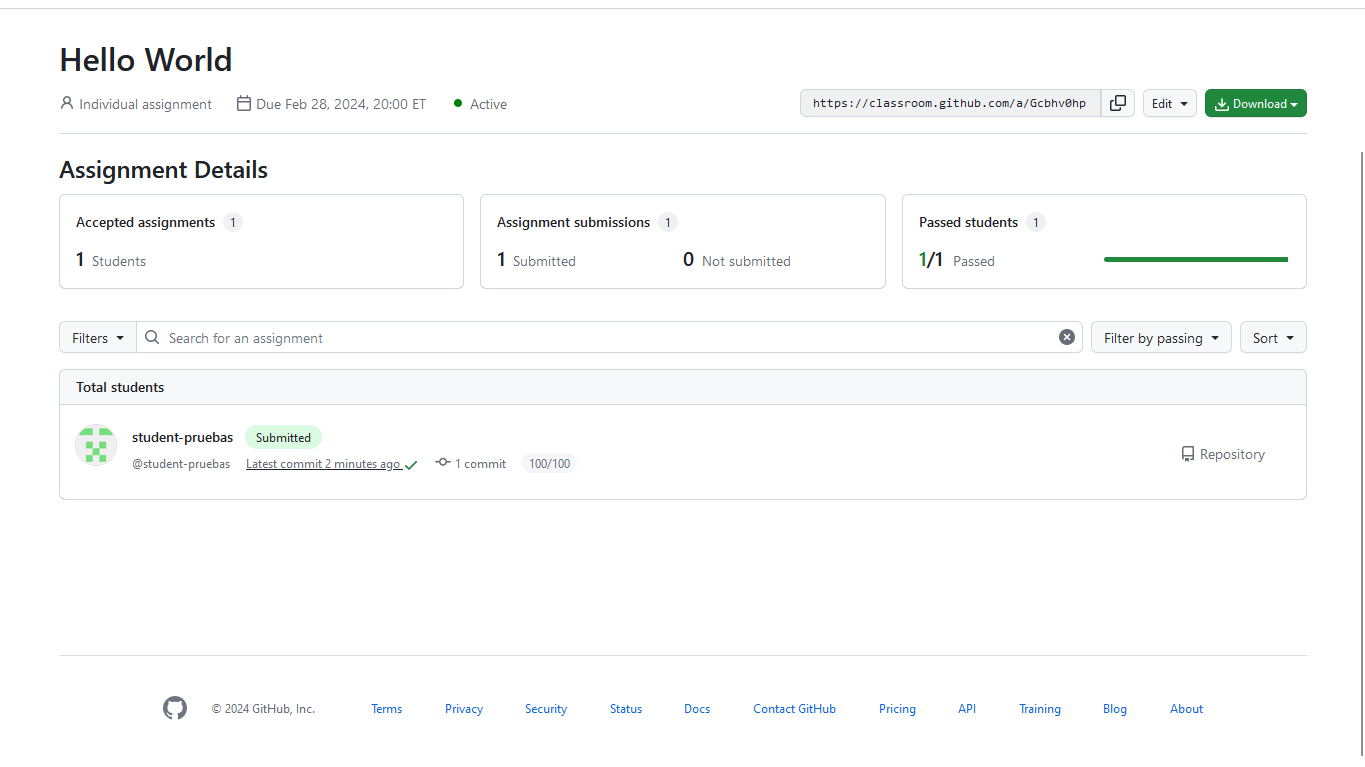
\includegraphics{unidades/unidad0/images/paste-15.png}
\end{center}

\begin{tcolorbox}[enhanced jigsaw, bottomrule=.15mm, rightrule=.15mm, colframe=quarto-callout-tip-color-frame, arc=.35mm, breakable, colbacktitle=quarto-callout-tip-color!10!white, toptitle=1mm, colback=white, opacitybacktitle=0.6, opacityback=0, bottomtitle=1mm, toprule=.15mm, titlerule=0mm, left=2mm, coltitle=black, leftrule=.75mm, title=\textcolor{quarto-callout-tip-color}{\faLightbulb}\hspace{0.5em}{Tip}]

\textbf{GitHub Classroom} ofrece una manera eficiente y organizada de
administrar tareas y asignaciones en entornos educativos, fomentando la
colaboración, el aprendizaje y la retroalimentación efectiva entre
profesores y estudiantes.

\end{tcolorbox}

\part{Unidad 1: Introducción e Instalaciones Necesarias}

\chapter{Introducción e Instalaciones
Necesarias.}\label{introducciuxf3n-e-instalaciones-necesarias.}

\begin{figure}[H]

{\centering 
\includegraphics{unidades/unidad1/images/logica_programacion.jpeg}

}

\caption{Lógica de la Programación}

\end{figure}%

En este Bootcamp aprenderemos las bases y fundamentos necesarios del
desarrollo web fullstack, esto es desde el frontend hasta el backend.

Para ello, utilizaremos Python como lenguaje de programación principal,
y Django y FastAPI como frameworks para el desarrollo de aplicaciones
web.

Por otra parte esta tambien el frontend, donde utilizaremos HTML, CSS y
JavaScript para el desarrollo de interfaces de usuario, aprenderemos
acerca de Node.js y React.js para el desarrollo de aplicaciones web del
lado del cliente.

Sin embargo antes de empezar con el desarrollo web, es necesario tener
una base sólida en programación, por lo que en este primer módulo
aprenderemos acerca de Python, un lenguaje de programación de alto
nivel, interpretado y orientado a objetos.

Por otra parte es necesario saber que cualquier lenguaje de programación
no es suficiente para poder desarrollar sistemas que permitan resolver
problemas del diario vivir, es necesario tener un entorno de desarrollo
adecuado, por lo que en este módulo también aprenderemos acerca de los
entornos de desarrollo que podemos utilizar para programar en Python.

En este módulo aprenderemos acerca de los siguientes temas:

\begin{itemize}
\item
  Introducción General a la Programación
\item
  Instalación de Python
\item
  Uso de REPL, PEP 8 y Zen de Python
\item
  Entornos de Desarrollo
\end{itemize}

\section{Introducción General a la
Programación}\label{introducciuxf3n-general-a-la-programaciuxf3n}

Si más preámbulos, empecemos con la introducción general a la
programación.

Es el proceso de diseñar e implementar un programa de computadora, es
decir, un conjunto de instrucciones que le dicen a una computadora qué
hacer.

Es una habilidad muy valiosa en el mundo actual, ya que la mayoría de
las tareas que realizamos a diario involucran el uso de computadoras y
software.

Nos permite automatizar tareas, resolver problemas de manera eficiente y
crear aplicaciones y sistemas que nos ayudan en nuestra vida diaria.

En este módulo aprenderemos los fundamentos de la programación
utilizando Python, un lenguaje de programación de alto nivel,
interpretado y orientado a objetos.

Antes de introducirnos en el aprendizaje del lenguaje de programación,
es importante conocer que debemos desarrollar la \textbf{lógica de la
prograamción}, es decir, la habilidad de pensar de manera lógica y
estructurada para resolver problemas de manera eficiente.

Analicemos el siguiente problema para entender la importancia de la
lógica de programación:

\begin{itemize}
\tightlist
\item
  \textbf{Problema}: Supongamos que queremos escribir un programa que
  imprima los números del 1 al 10.
\end{itemize}

¿Cómo resolverías este problema?

Una posible solución sería escribir un programa que imprima los números
del 1 al 10 de manera secuencial.

\begin{Shaded}
\begin{Highlighting}[]
\BuiltInTok{print}\NormalTok{(}\DecValTok{1}\NormalTok{)}
\BuiltInTok{print}\NormalTok{(}\DecValTok{2}\NormalTok{)}
\BuiltInTok{print}\NormalTok{(}\DecValTok{3}\NormalTok{)}
\BuiltInTok{print}\NormalTok{(}\DecValTok{4}\NormalTok{)}
\BuiltInTok{print}\NormalTok{(}\DecValTok{5}\NormalTok{)}
\BuiltInTok{print}\NormalTok{(}\DecValTok{6}\NormalTok{)}
\BuiltInTok{print}\NormalTok{(}\DecValTok{7}\NormalTok{)}
\BuiltInTok{print}\NormalTok{(}\DecValTok{8}\NormalTok{)}
\BuiltInTok{print}\NormalTok{(}\DecValTok{9}\NormalTok{)}
\BuiltInTok{print}\NormalTok{(}\DecValTok{10}\NormalTok{)}
\end{Highlighting}
\end{Shaded}

En el ejemplo anterior, hemos resuelto el problema de imprimir los
números del 1 al 10 de manera secuencial. Sin embargo, esta solución no
es escalable, ya que si quisiéramos imprimir los números del 1 al 1000,
tendríamos que escribir 1000 instrucciones de impresión.

Una solución más eficiente sería utilizar un bucle para imprimir los
números del 1 al 10 de manera automática.

\begin{Shaded}
\begin{Highlighting}[]
\ControlFlowTok{for}\NormalTok{ i }\KeywordTok{in} \BuiltInTok{range}\NormalTok{(}\DecValTok{1}\NormalTok{, }\DecValTok{11}\NormalTok{):}
    \BuiltInTok{print}\NormalTok{(i)}
\end{Highlighting}
\end{Shaded}

En el ejemplo anterior, hemos utilizado un bucle \textbf{for} para
imprimir los números del 1 al 10 de manera automática. Esta solución es
más eficiente y escalable, ya que podemos cambiar el rango del bucle
para imprimir los números del 1 al 1000 sin tener que modificar el
código.

\begin{itemize}
\tightlist
\item
  \textbf{Problema}: Supongamos que queremos escribir un programa que
  imprima un saludo personalizado.
\end{itemize}

¿Cómo resolverías este problema?

Una posible solución sería escribir un programa que solicite al usuario
su nombre y luego imprima un saludo personalizado.

\begin{Shaded}
\begin{Highlighting}[]
\NormalTok{name }\OperatorTok{=} \BuiltInTok{input}\NormalTok{(}\StringTok{"Ingrese su nombre: "}\NormalTok{)}
\BuiltInTok{print}\NormalTok{(}\StringTok{"Hola, "} \OperatorTok{+}\NormalTok{ name }\OperatorTok{+} \StringTok{"!"}\NormalTok{)}
\end{Highlighting}
\end{Shaded}

En el ejemplo anterior, hemos resuelto el problema de imprimir un saludo
personalizado solicitando al usuario su nombre. Esta solución es
interactiva y personalizada, ya que el saludo se adapta al nombre del
usuario.

En resumen, la lógica de programación es la habilidad de pensar de
manera lógica y estructurada para resolver problemas de manera
eficiente. Es fundamental para desarrollar programas y sistemas que nos
ayuden en nuestra vida diaria.

A continuación te ofresco algunas páginas que puedes revisar por tu
cuenta y que te permitirán practicar el desarrollo de la lógica de
programación:

\begin{itemize}
\tightlist
\item
  \href{https://www.hackerrank.com/}{HackerRank}
\item
  \href{https://leetcode.com/}{LeetCode}
\item
  \href{https://retosdeprogramacion.com}{Retod de Programación}
\item
  \href{https://www.geeksforgeeks.org/}{Geeks for Geeks}
\end{itemize}

\section{Instalación de Python}\label{instalaciuxf3n-de-python}

\begin{figure}[H]

{\centering 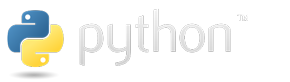
\includegraphics{index_files/mediabag/python-logo.png}

}

\caption{Python}

\end{figure}%

Para instalar Python en tu computadora, sigue los siguientes pasos:

\begin{enumerate}
\def\labelenumi{\arabic{enumi}.}
\tightlist
\item
  Ve al sitio web oficial de Python en \url{https://www.python.org/}.
\end{enumerate}

\begin{figure}[H]

{\centering 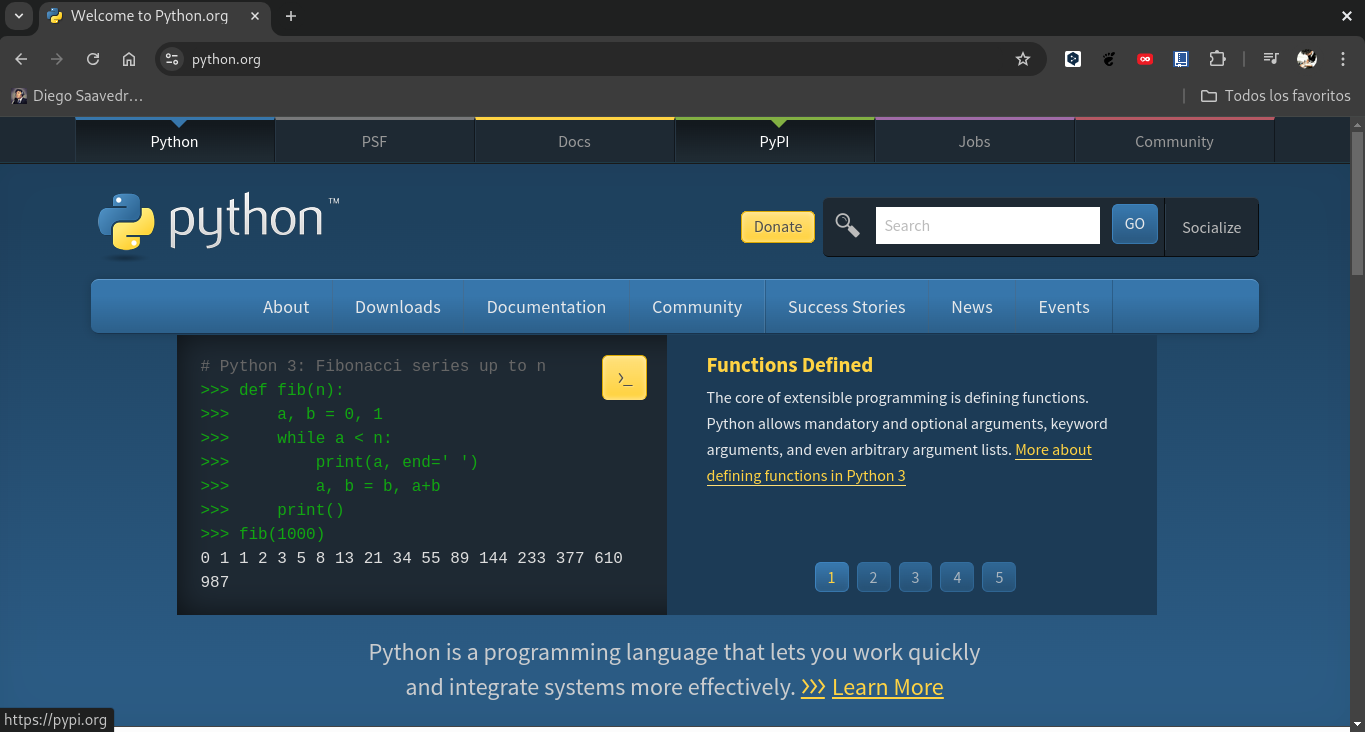
\includegraphics{unidades/unidad1/images/python.org.png}

}

\caption{Python}

\end{figure}%

\begin{enumerate}
\def\labelenumi{\arabic{enumi}.}
\setcounter{enumi}{1}
\tightlist
\item
  Haz clic en el botón de descarga de Python.
\end{enumerate}

\begin{figure}[H]

{\centering 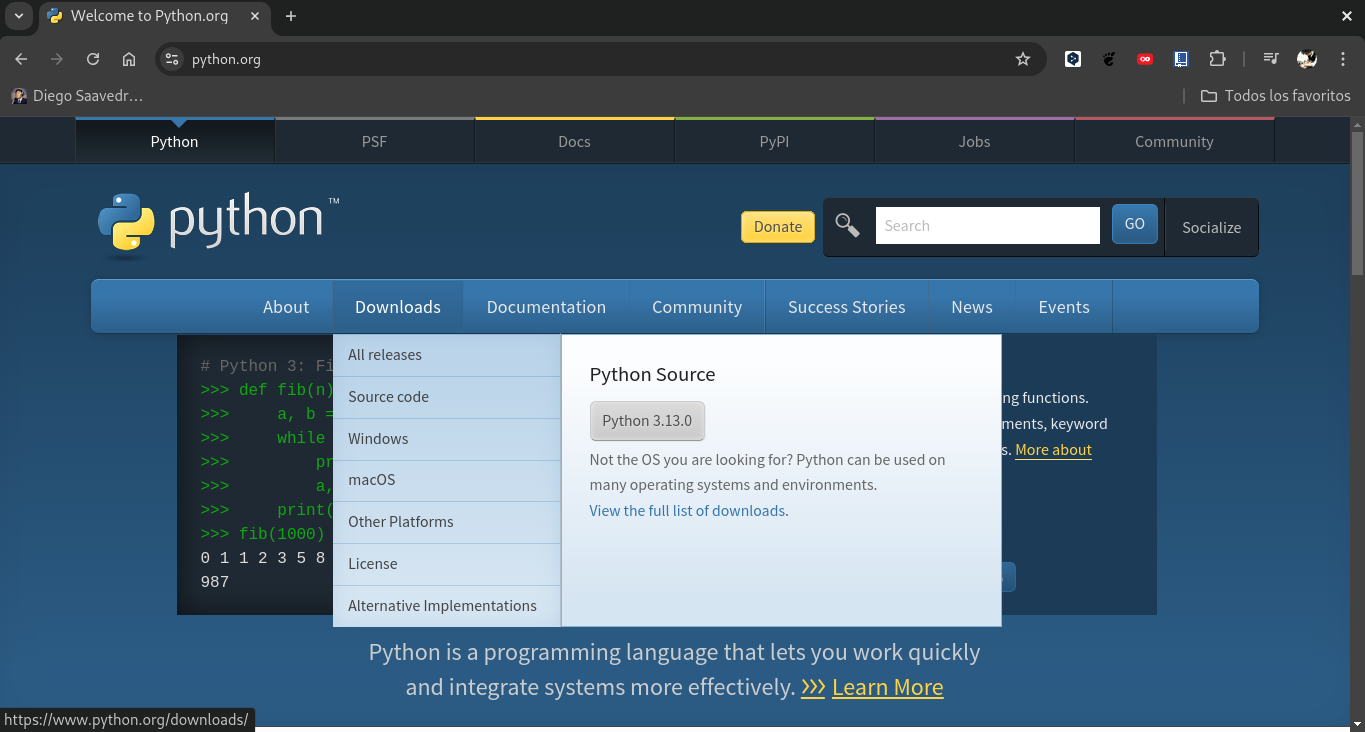
\includegraphics{unidades/unidad1/images/download.png}

}

\caption{Python}

\end{figure}%

\begin{enumerate}
\def\labelenumi{\arabic{enumi}.}
\setcounter{enumi}{2}
\item
  Selecciona la versión de Python que deseas instalar (recomendamos la
  versión más reciente).
\item
  Descarga el instalador de Python para tu sistema operativo (Windows,
  macOS o Linux).
\end{enumerate}

\begin{figure}[H]

{\centering 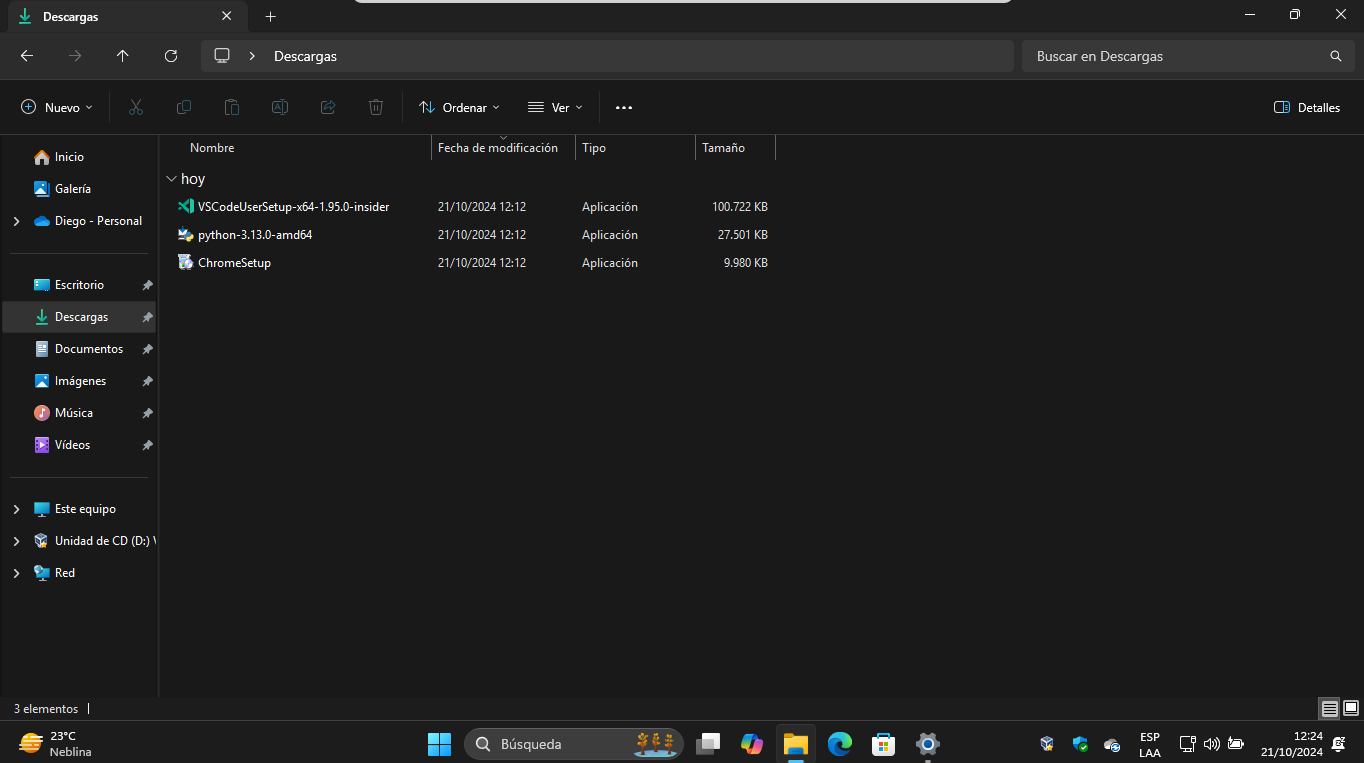
\includegraphics{unidades/unidad1/images/instalador_python.png}

}

\caption{Python}

\end{figure}%

\begin{enumerate}
\def\labelenumi{\arabic{enumi}.}
\setcounter{enumi}{4}
\tightlist
\item
  Ejecuta el instalador de Python y sigue las instrucciones en pantalla
  para completar la instalación.
\end{enumerate}

\begin{figure}[H]

{\centering 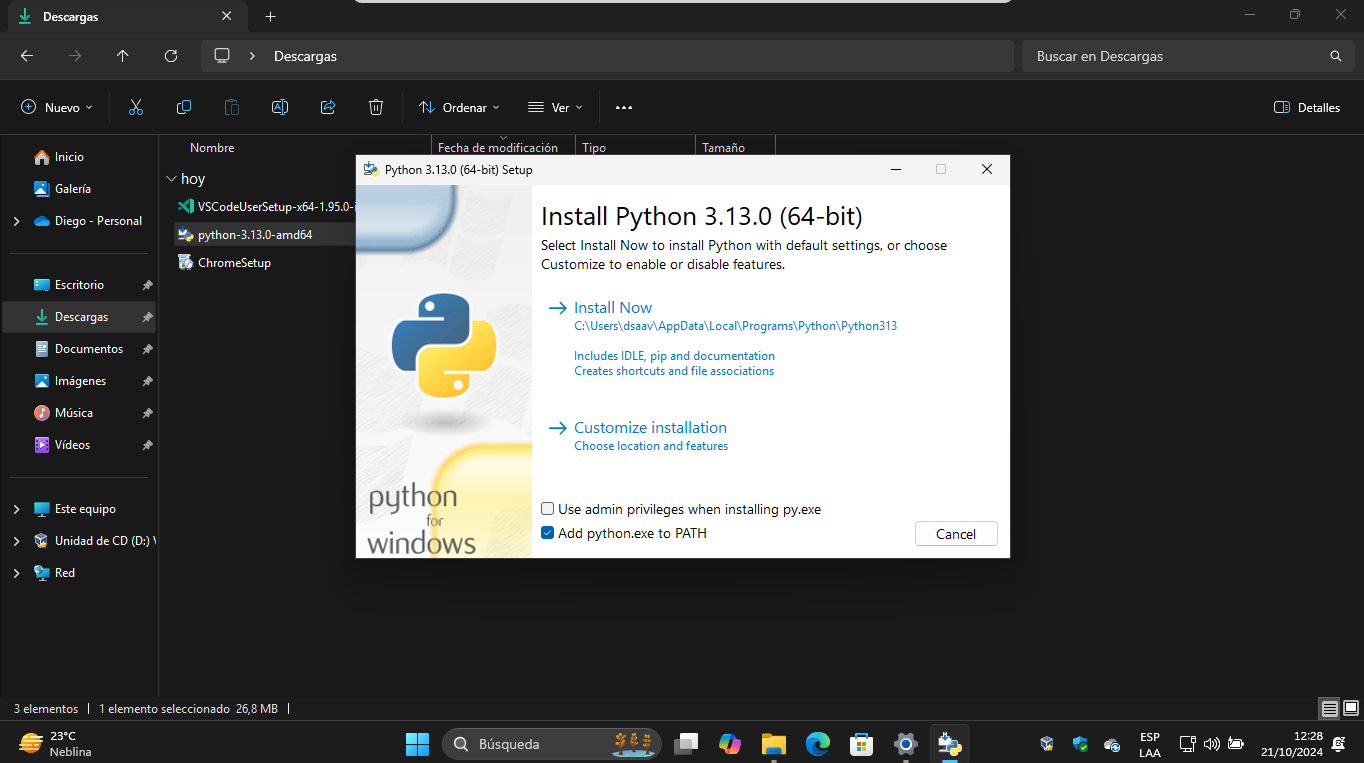
\includegraphics{unidades/unidad1/images/add_to_path.png}

}

\caption{Python}

\end{figure}%

Una vez que hayas instalado Python en tu computadora, puedes verificar
que la instalación se haya realizado correctamente abriendo una terminal
y ejecutando el siguiente comando:

\begin{figure}[H]

{\centering 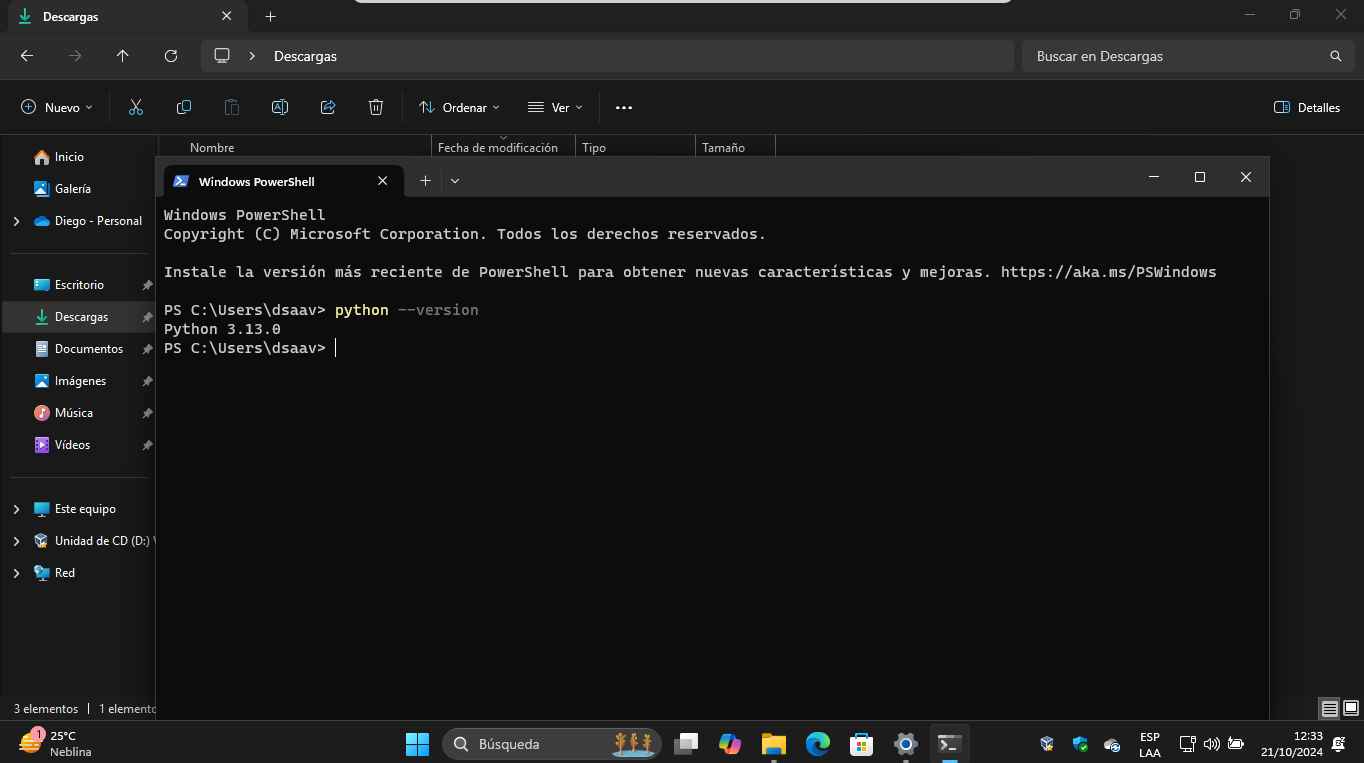
\includegraphics{unidades/unidad1/images/python_version.png}

}

\caption{Python}

\end{figure}%

\begin{Shaded}
\begin{Highlighting}[]
\ExtensionTok{python} \AttributeTok{{-}{-}version}
\end{Highlighting}
\end{Shaded}

Si la instalación se realizó correctamente, verás la versión de Python
instalada en tu computadora.

\section{Uso de REPL, PEP 8 y Zen de
Python}\label{uso-de-repl-pep-8-y-zen-de-python}

En esta sección, aprenderemos acerca de REPL, PEP 8 y Zen de Python.

\subsection{REPL}\label{repl}

REPL (Read-Eval-Print Loop) es un entorno interactivo que permite
escribir y ejecutar código de Python de manera interactiva. Es una
excelente herramienta para probar y experimentar con el lenguaje de
programación.

Para abrir el REPL de Python, abre una terminal y ejecuta el siguiente
comando:

\begin{Shaded}
\begin{Highlighting}[]
\ExtensionTok{python}
\end{Highlighting}
\end{Shaded}

Una vez que hayas abierto el REPL de Python, puedes escribir y ejecutar
código de Python de manera interactiva. Por ejemplo, puedes escribir una
expresión matemática y ver el resultado:

\begin{Shaded}
\begin{Highlighting}[]
\OperatorTok{\textgreater{}\textgreater{}\textgreater{}} \DecValTok{2} \OperatorTok{+} \DecValTok{2}
\OperatorTok{\textgreater{}\textgreater{}\textgreater{}} \DecValTok{4}
\OperatorTok{\textgreater{}\textgreater{}\textgreater{}} \DecValTok{3} \OperatorTok{*} \DecValTok{4}
\OperatorTok{\textgreater{}\textgreater{}\textgreater{}} \DecValTok{12}
\OperatorTok{\textgreater{}\textgreater{}\textgreater{}} \DecValTok{10} \OperatorTok{/} \DecValTok{2}
\OperatorTok{\textgreater{}\textgreater{}\textgreater{}} \FloatTok{5.0}
\OperatorTok{\textgreater{}\textgreater{}\textgreater{}} \DecValTok{2} \OperatorTok{**} \DecValTok{3}
\OperatorTok{\textgreater{}\textgreater{}\textgreater{}} \DecValTok{8}
\OperatorTok{\textgreater{}\textgreater{}\textgreater{}} \StringTok{"Hola, Mundo!"}
\OperatorTok{\textgreater{}\textgreater{}\textgreater{}} \StringTok{\textquotesingle{}Hola, Mundo!\textquotesingle{}}
\OperatorTok{\textgreater{}\textgreater{}\textgreater{}} \StringTok{"Hola, "} \OperatorTok{+} \StringTok{"Mundo!"}
\OperatorTok{\textgreater{}\textgreater{}\textgreater{}} \StringTok{\textquotesingle{}Hola, \textquotesingle{}} \OperatorTok{*} \DecValTok{3}
\OperatorTok{\textgreater{}\textgreater{}\textgreater{}} \StringTok{\textquotesingle{}Hola, Hola, Hola, \textquotesingle{}}
\OperatorTok{\textgreater{}\textgreater{}\textgreater{}} \BuiltInTok{print}\NormalTok{(}\StringTok{"Hola, Mundo!"}\NormalTok{)}
\OperatorTok{\textgreater{}\textgreater{}\textgreater{}}\NormalTok{ Hola, Mundo}\OperatorTok{!}
\end{Highlighting}
\end{Shaded}

\chapter{Pep 8}\label{pep-8}

PEP 8 (Python Enhancement Proposal 8) es una guía de estilo para
escribir código de Python de manera clara y legible. Es una excelente
referencia para seguir buenas prácticas de codificación y mantener un
código limpio y ordenado.

Algunas recomendaciones de PEP 8 son:

\begin{itemize}
\item
  Utiliza sangrías de 4 espacios para indentar el código.
\item
  Utiliza líneas en blanco para separar funciones y clases.
\item
  Utiliza nombres descriptivos para las variables y funciones.
\item
  Utiliza comentarios para explicar el código y hacerlo más legible.
\item
  Utiliza espacios alrededor de los operadores y después de las comas.
\item
  Utiliza comillas simples o dobles de manera consistente para las
  cadenas de texto.
\item
  Utiliza la función \textbf{print()} para imprimir en la consola.
\end{itemize}

\chapter{Zen de python.}\label{zen-de-python.}

El Zen de Python es una colección de 19 aforismos que resumen los
principios de diseño y filosofía de Python. Fueron escritos por Tim
Peters, uno de los desarrolladores originales de Python, y se pueden ver
en cualquier instalación de Python utilizando el siguiente comando:

\begin{Shaded}
\begin{Highlighting}[]
\ExtensionTok{import}\NormalTok{ this}
\end{Highlighting}
\end{Shaded}

Algunos de los aforismos más conocidos del Zen de Python son:

\begin{itemize}
\item
  Hermoso es mejor que feo.
\item
  Explícito es mejor que implícito.
\item
  Simple es mejor que complejo.
\item
  Complejo es mejor que complicado.
\item
  La legibilidad cuenta.
\item
  Los casos especiales no son lo suficientemente especiales como para
  romper las reglas.
\item
  Si la implementación es difícil de explicar, es una mala idea.
\item
  Si la implementación es fácil de explicar, puede que sea una buena
  idea.
\item
  Los errores nunca deberían pasar en silencio.
\item
  A menos que sean silenciados.
\item
  En la cara de la ambigüedad, rechaza la tentación de adivinar.
\item
  Debería haber una, y preferiblemente solo una, manera obvia de
  hacerlo.
\item
  Aunque esa manera puede no ser obvia al principio a menos que seas
  holandés.
\end{itemize}

En el ejemplo anterior, hemos utilizado el REPL de Python para ejecutar
expresiones matemáticas y cadenas de texto. Es una excelente manera de
probar y experimentar con el lenguaje de programación.

\section{Entornos de Desarrollo}\label{entornos-de-desarrollo}

Un entorno de desarrollo es un conjunto de herramientas que nos permiten
escribir, depurar y ejecutar código de manera eficiente. Es fundamental
para desarrollar programas y sistemas de manera efectiva.

Existen varios entornos de desarrollo que podemos utilizar para
programar en Python. Algunos de los más populares son:

\begin{itemize}
\tightlist
\item
  \textbf{IDLE}: Es el entorno de desarrollo integrado (IDE) oficial de
  Python. Viene incluido con la instalación de Python y es una excelente
  opción para programar en Python.
\end{itemize}

\begin{figure}[H]

{\centering 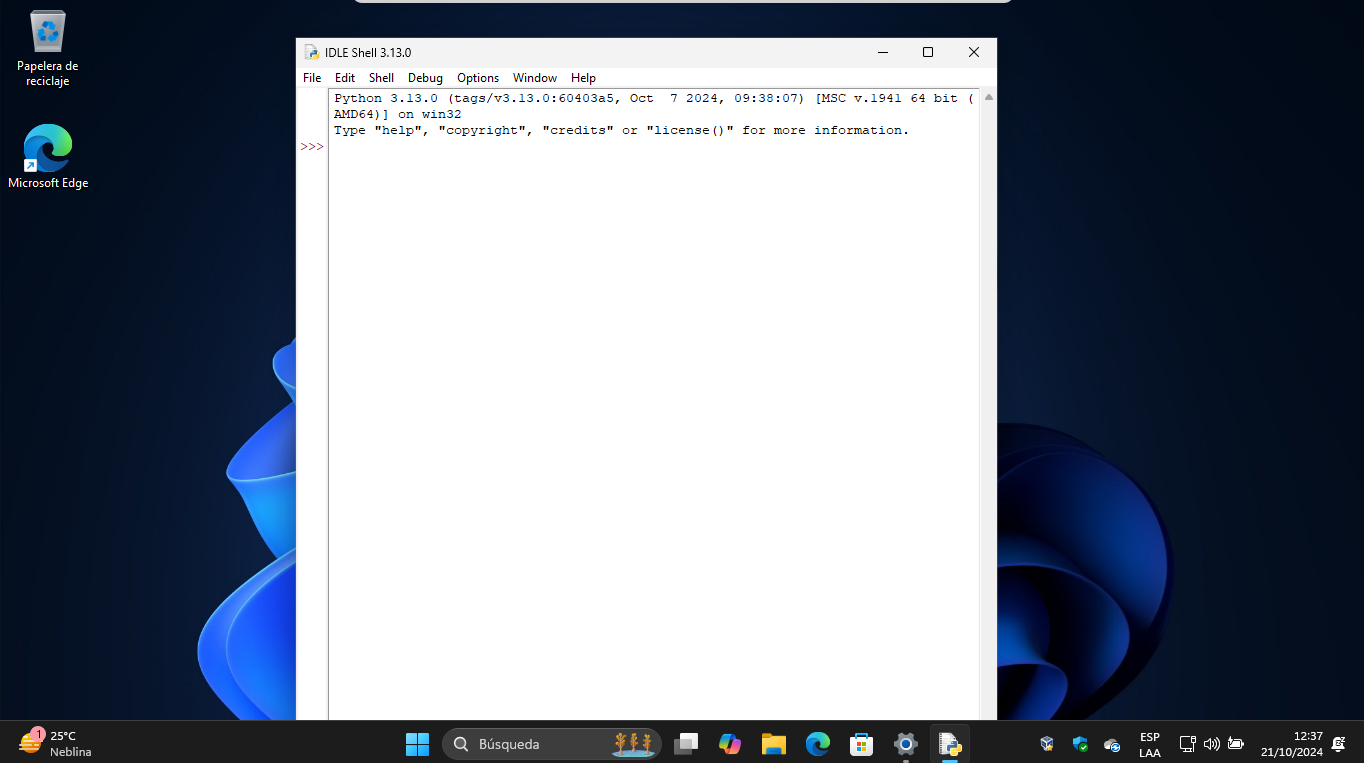
\includegraphics{unidades/unidad1/images/idle_python.png}

}

\caption{IDLE}

\end{figure}%

\begin{itemize}
\tightlist
\item
  \textbf{PyCharm}: Es un IDE de Python desarrollado por JetBrains. Es
  una excelente opción para programar en Python, ya que ofrece muchas
  características y herramientas útiles.
\end{itemize}

\begin{figure}[H]

{\centering 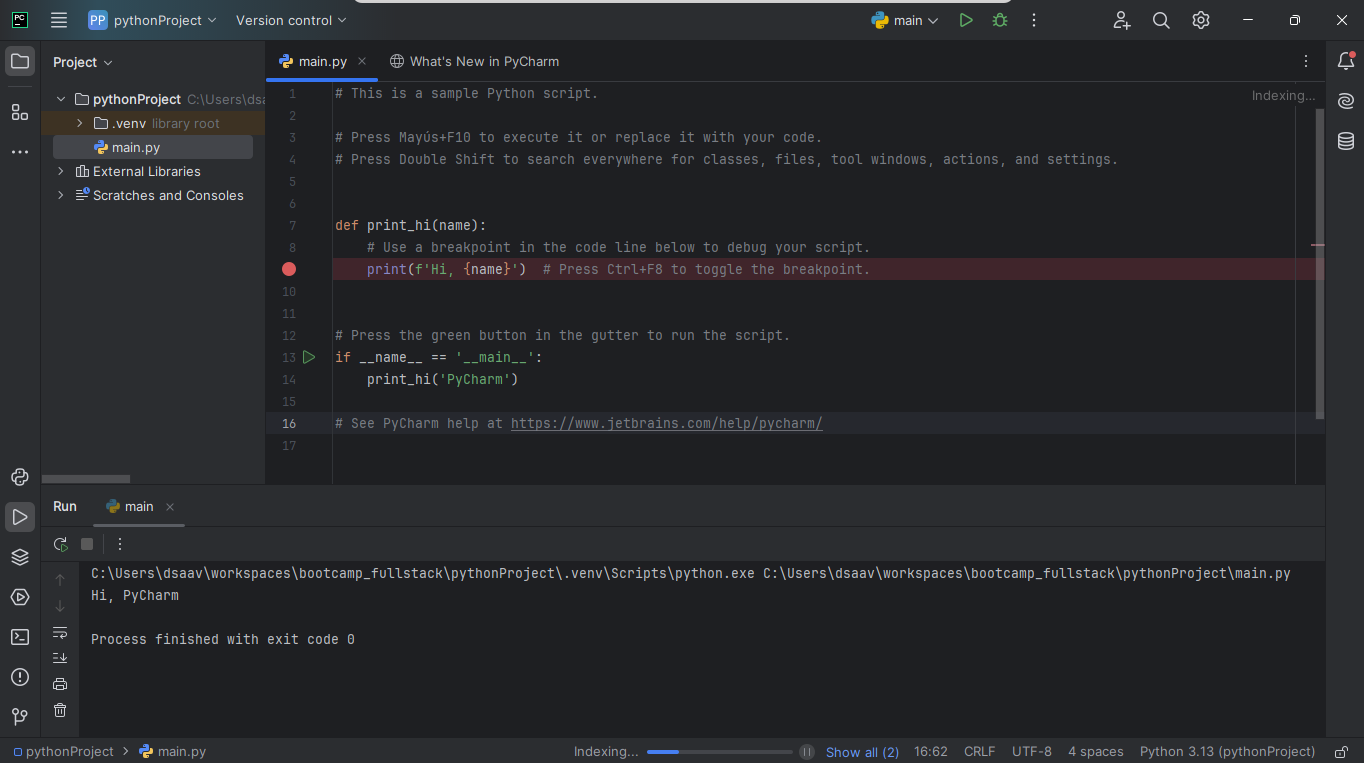
\includegraphics{unidades/unidad1/images/pycharm.png}

}

\caption{PyCharm}

\end{figure}%

\begin{itemize}
\tightlist
\item
  \textbf{Visual Studio Code}: Es un editor de código desarrollado por
  Microsoft. Es una excelente opción para programar en Python, ya que
  ofrece muchas extensiones y herramientas útiles.
\end{itemize}

\begin{figure}[H]

{\centering 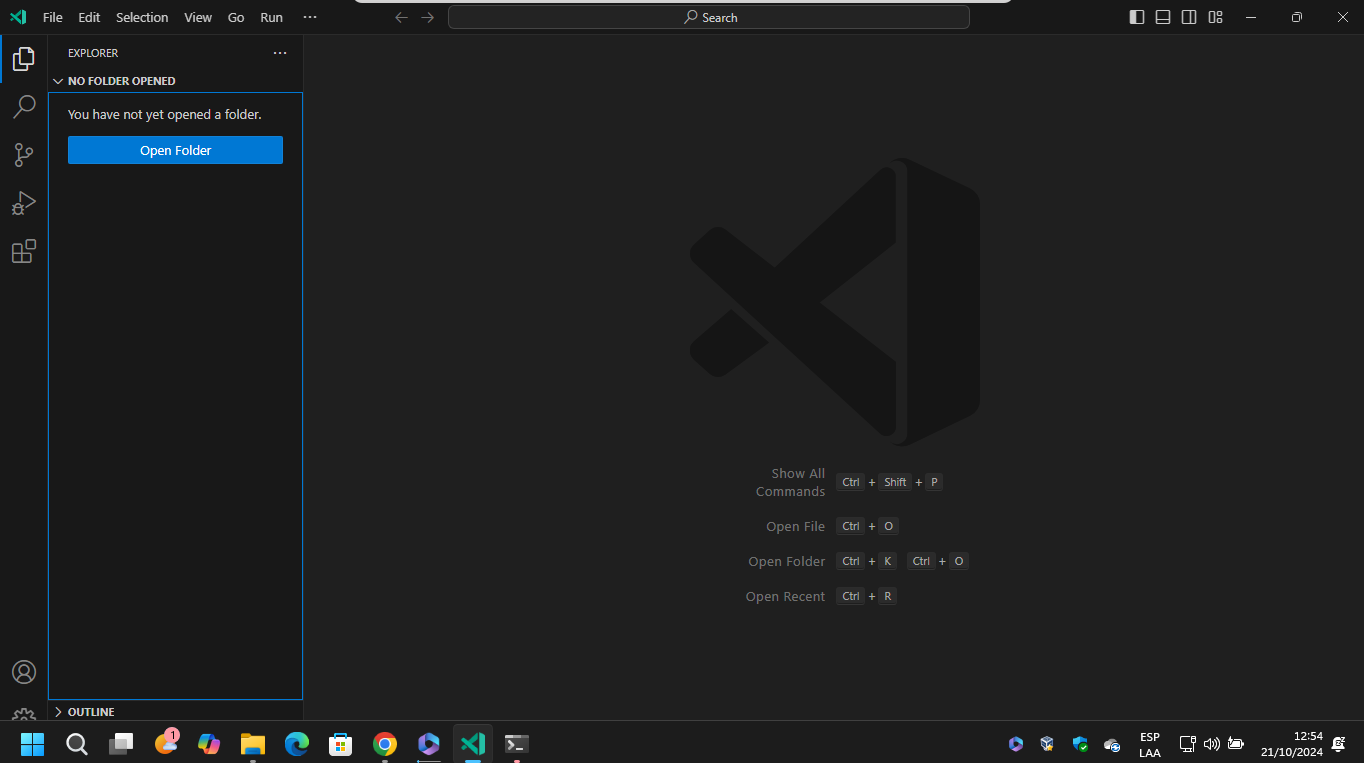
\includegraphics{unidades/unidad1/images/vscode.png}

}

\caption{Visual Studio Code}

\end{figure}%

\begin{itemize}
\tightlist
\item
  \textbf{Jupyter Notebook}: Es una aplicación web que nos permite crear
  y compartir documentos interactivos que contienen código de Python,
  visualizaciones y texto explicativo.
\end{itemize}

\begin{figure}[H]

{\centering 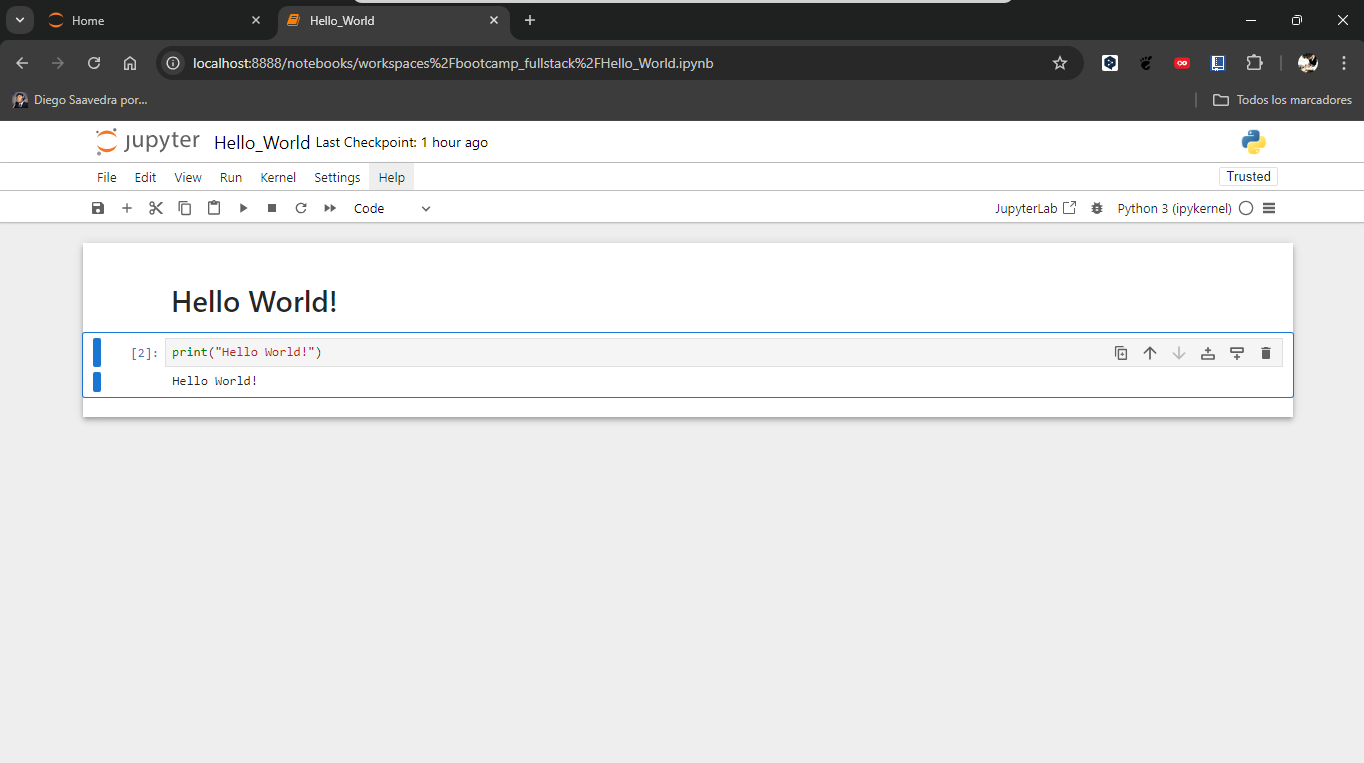
\includegraphics{unidades/unidad1/images/jupyter_notebook.png}

}

\caption{Jupyter Notebook}

\end{figure}%

En este bootcam utilizaremos \textbf{Visual Studio Code} como editor de
código para programar en Python. Sin embargo, te recomiendo que explores
otros entornos de desarrollo y elijas el que mejor se adapte a tus
necesidades y preferencias.

\section{5 Consejos para mejorar la lógica de
programación.}\label{consejos-para-mejorar-la-luxf3gica-de-programaciuxf3n.}

\begin{enumerate}
\def\labelenumi{\arabic{enumi}.}
\item
  \textbf{Practica regularmente}: La práctica es fundamental para
  mejorar la lógica de programación. Dedica tiempo a resolver problemas
  de programación y desafíos lógicos de manera regular.
\item
  \textbf{Descompón el problema}: Divide los problemas complejos en
  problemas más pequeños y manejables. Esto te ayudará a abordar el
  problema de manera más efectiva y eficiente.
\item
  \textbf{Utiliza pseudocódigo}: Antes de escribir código, utiliza
  pseudocódigo para planificar y diseñar tu solución. Esto te ayudará a
  visualizar el problema y encontrar una solución más clara.
\item
  \textbf{Comenta tu código}: Utiliza comentarios para explicar tu
  código y hacerlo más legible. Esto te ayudará a entender tu código y a
  identificar posibles errores.
\item
  \textbf{Colabora con otros}: Trabaja en equipo con otros programadores
  para resolver problemas de programación. La colaboración te permitirá
  aprender de otros y mejorar tus habilidades de programación.
\end{enumerate}

¡Espero que estos consejos te sean útiles para mejorar tu lógica de
programación!

\section{Conclusiones}\label{conclusiones}

En este módulo hemos aprendido acerca de la introducción general a la
programación, la instalación de Python, el uso de REPL, PEP 8 y Zen de
Python, y los entornos de desarrollo que podemos utilizar para programar
en Python.

\chapter{Introducción a la Programación con
Python}\label{introducciuxf3n-a-la-programaciuxf3n-con-python}

\begin{figure}[H]

{\centering 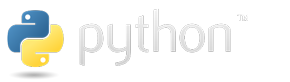
\includegraphics{index_files/mediabag/python-logo.png}

}

\caption{Python}

\end{figure}%

\section{¿Qué es la programación?}\label{quuxe9-es-la-programaciuxf3n}

La programación es el proceso de diseñar e implementar un programa de
computadora. Un programa es un conjunto de instrucciones que le dice a
la computadora qué hacer. Estas instrucciones pueden ser escritas en
diferentes lenguajes de programación, como Python, Java, C++, entre
otros.

\section{¿Qué es Python?}\label{quuxe9-es-python}

Python es un lenguaje de programación de alto nivel, interpretado y
orientado a objetos. Fue creado por Guido van Rossum en 1991 y es uno de
los lenguajes de programación más populares en la actualidad. Python es
conocido por su sintaxis simple y legible, lo que lo hace ideal para
principiantes en programación.

\section{¿Por qué aprender Python?}\label{por-quuxe9-aprender-python}

Python es un lenguaje de programación versátil que se puede utilizar
para una amplia variedad de aplicaciones, como desarrollo web, análisis
de datos, inteligencia artificial, entre otros. Además, Python es fácil
de aprender y de usar, lo que lo convierte en una excelente opción para
aquellos que quieren iniciarse en la programación.

\section{¿Qué aprenderemos en este
bootcamp?}\label{quuxe9-aprenderemos-en-este-bootcamp}

En este bootcamp aprenderemos los conceptos básicos de programación con
Python, incluyendo variables, tipos de datos, operadores, estructuras de
control, funciones, entre otros. Al final del bootcamp, tendrás los
conocimientos necesarios para crear tus propios programas en Python y
continuar tu aprendizaje en programación.

¡Vamos a empezar!

\section{Identación en Python}\label{identaciuxf3n-en-python}

Python utiliza la identación para definir bloques de código. La
identación es el espacio en blanco al principio de una línea de código y
se utiliza para indicar que una línea de código pertenece a un bloque de
código. Por ejemplo, en el siguiente código, la línea
\textbf{print(``Hola, mundo!'')} está identada con cuatro espacios, lo
que indica que pertenece al bloque de código del \textbf{if}.

\begin{Shaded}
\begin{Highlighting}[]
\ControlFlowTok{if} \VariableTok{True}\NormalTok{:}
    \BuiltInTok{print}\NormalTok{(}\StringTok{"Hola, mundo!"}\NormalTok{)}
\end{Highlighting}
\end{Shaded}

En el código anterior, la línea \textbf{print(``Hola, mundo!'')} se
ejecutará si la condición del \textbf{if} es verdadera. Si la línea no
estuviera identada, no se ejecutaría dentro del bloque de código del
\textbf{if}.

\section{Comentarios en python}\label{comentarios-en-python}

Los comentarios son líneas de texto que se utilizan para explicar el
código y hacerlo más legible. En Python, los comentarios se crean
utilizando el símbolo \textbf{\#}. Todo lo que sigue al símbolo
\textbf{\#} en una línea se considera un comentario y no se ejecuta como
código.

\begin{Shaded}
\begin{Highlighting}[]
\CommentTok{\# Este es un comentarios}
\BuiltInTok{print}\NormalTok{(}\StringTok{"Hola, mundo!"}\NormalTok{) }\CommentTok{\# Este es otro comentarios}
\end{Highlighting}
\end{Shaded}

En el código anterior, la línea \textbf{print(``Hola, mundo!'')} se
ejecutará, pero los comentarios no se ejecutarán.

\section{Variables y Variables
Múltiples}\label{variables-y-variables-muxfaltiples}

Una variable es un contenedor que se utiliza para almacenar datos en un
programa. En Python, una variable se crea asignando un valor a un nombre
de variable. Por ejemplo, en el siguiente código, la variable
\textbf{nombre} se crea y se le asigna el valor \textbf{``Juan''}.

\begin{Shaded}
\begin{Highlighting}[]
\NormalTok{nombre }\OperatorTok{=} \StringTok{"Juan"}
\BuiltInTok{print}\NormalTok{(nombre)}
\end{Highlighting}
\end{Shaded}

En el código anterior, la variable \textbf{nombre} se imprime en la
consola y se muestra el valor \textbf{``Juan''}.

En Python, también se pueden crear múltiples variables en una sola
línea. Por ejemplo, en el siguiente código, se crean tres variables
\textbf{a}, \textbf{b} y \textbf{c} y se les asignan los valores
\textbf{1}, \textbf{2} y \textbf{3} respectivamente.

\begin{Shaded}
\begin{Highlighting}[]
\NormalTok{a, b, c }\OperatorTok{=} \DecValTok{1}\NormalTok{, }\DecValTok{2}\NormalTok{, }\DecValTok{3}
\BuiltInTok{print}\NormalTok{(a, b, c)}
\end{Highlighting}
\end{Shaded}

En el código anterior, las variables \textbf{a}, \textbf{b} y \textbf{c}
se imprimen en la consola y se muestran los valores \textbf{1},
\textbf{2} y \textbf{3} respectivamente.

\section{Concatenación de Cadenas}\label{concatenaciuxf3n-de-cadenas}

La concatenación de cadenas es la unión de dos o más cadenas en una sola
cadena. En Python, se puede concatenar cadenas utilizando el operador
\textbf{+}. Por ejemplo, en el siguiente código, se concatenan las
cadenas \textbf{``Hola''} y \textbf{``mundo''} en una sola cadena.

\begin{Shaded}
\begin{Highlighting}[]
\NormalTok{saludo }\OperatorTok{=} \StringTok{"Hola"} \OperatorTok{+} \StringTok{"mundo"}
\BuiltInTok{print}\NormalTok{(saludo)}
\end{Highlighting}
\end{Shaded}

En el código anterior, la variable \textbf{saludo} se imprime en la
consola y se muestra la cadena \textbf{``Hola mundo''}.

Algunos ejemplos adicionales de concatenación de cadenas son:

\begin{Shaded}
\begin{Highlighting}[]
\NormalTok{nombre }\OperatorTok{=} \StringTok{"Juan"}
\NormalTok{apellido }\OperatorTok{=} \StringTok{"Pérez"}
\NormalTok{nombre\_completo }\OperatorTok{=}\NormalTok{ nombre }\OperatorTok{+} \StringTok{" "} \OperatorTok{+}\NormalTok{ apellido}
\BuiltInTok{print}\NormalTok{(nombre\_completo)}
\end{Highlighting}
\end{Shaded}

En el código anterior, la variable \textbf{nombre\_completo} se imprime
en la consola y se muestra la cadena \textbf{``Juan Pérez''}.

\begin{Shaded}
\begin{Highlighting}[]
\NormalTok{edad }\OperatorTok{=} \DecValTok{30}
\NormalTok{mensaje }\OperatorTok{=} \StringTok{"Tengo "} \OperatorTok{+} \BuiltInTok{str}\NormalTok{(edad) }\OperatorTok{+} \StringTok{" años"}
\BuiltInTok{print}\NormalTok{(mensaje)}
\end{Highlighting}
\end{Shaded}

En el código anterior, la variable \textbf{mensaje} se imprime en la
consola y se muestra la cadena \textbf{``Tengo 30 años''}.

\chapter{Actividad}\label{actividad}

\section{instrucciones}\label{instrucciones}

\begin{enumerate}
\def\labelenumi{\arabic{enumi}.}
\item
  Crea una variable llamada \textbf{nombre} y asígnale tu nombre.
\item
  Crea una variable llamada \textbf{edad} y asígnale tu edad.
\item
  Crea una variable llamada \textbf{ciudad} y asígnale tu ciudad de
  origen.
\item
  Imprime en la consola un mensaje que contenga tu nombre, edad y ciudad
  de origen utilizando la concatenación de cadenas.
\item
  Crea una variable llamada \textbf{mensaje} y asígnale el siguiente
  mensaje: ``Hola, mi nombre es {[}nombre{]}, tengo {[}edad{]} años y
  soy de {[}ciudad{]}.''
\item
  Imprime en la consola el mensaje utilizando la variable
  \textbf{mensaje}.
\end{enumerate}

🔍 Pistas

\begin{itemize}
\tightlist
\item
  Para concatenar cadenas en Python, utiliza el operador \textbf{+}.

  \begin{itemize}
  \tightlist
  \item
    Para convertir un número entero en una cadena, utiliza la función
    \textbf{str()}.
  \end{itemize}
\end{itemize}

\chapter{Conclusión}\label{conclusiuxf3n-1}

En este módulo, aprendimos los conceptos básicos de programación con
Python, incluyendo variables, identación, comentarios y concatenación de
cadenas. Estos conceptos son fundamentales para comprender y escribir
programas en Python. En los módulos siguientes, profundizaremos en otros
aspectos de la programación con Python, como tipos de datos, operadores,
estructuras de control, funciones, entre otros. ¡Sigue adelante!

\chapter{Tipos de Datos}\label{tipos-de-datos}

\begin{figure}[H]

{\centering 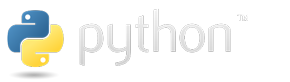
\includegraphics{index_files/mediabag/python-logo.png}

}

\caption{Python}

\end{figure}%

Los tipos de Datos en Python son la forma en que Python clasifica y
almacena los datos. Los tipos de datos más comunes en Python son:

\begin{itemize}
\tightlist
\item
  Números
\item
  Cadenas
\item
  Listas
\item
  Tuplas
\item
  Diccionarios
\item
  Booleanos
\item
  Rango
\end{itemize}

En esta actividad, aprenderás sobre los diferentes tipos de datos en
Python y cómo se utilizan.

\section{String y Números.}\label{string-y-nuxfameros.}

Los String y los Números son dos de los tipos de datos más comunes en
Python. Los String son secuencias de caracteres, como letras, números y
símbolos, que se utilizan para representar texto. Los Números, por otro
lado, son valores numéricos, como enteros y decimales, que se utilizan
para realizar cálculos matemáticos.

\subsection{String}\label{string}

Los String en Python se crean utilizando comillas simples \textbf{' '} o
comillas dobles \textbf{'' ``}. Por ejemplo:

\begin{Shaded}
\begin{Highlighting}[]
\NormalTok{nombre }\OperatorTok{=} \StringTok{"Juan"}
\NormalTok{apellido }\OperatorTok{=} \StringTok{\textquotesingle{}Pérez\textquotesingle{}}
\end{Highlighting}
\end{Shaded}

En el código anterior, se crean dos variables, \textbf{nombre} y
\textbf{apellido}, que contienen los String \textbf{``Juan''} y
\textbf{``Pérez''} respectivamente.

\subsection{Números}\label{nuxfameros}

Los Números en Python pueden ser enteros o decimales. Los enteros son
números enteros, como \textbf{1}, \textbf{2}, \textbf{3}, mientras que
los decimales son números con decimales, como \textbf{1.5},
\textbf{2.75}, \textbf{3.14}. Por ejemplo:

\begin{Shaded}
\begin{Highlighting}[]
\NormalTok{entero }\OperatorTok{=} \DecValTok{10}
\NormalTok{decimal }\OperatorTok{=} \FloatTok{3.14}
\end{Highlighting}
\end{Shaded}

En el código anterior, se crean dos variables, \textbf{entero} y
\textbf{decimal}, que contienen los números \textbf{10} y \textbf{3.14}
respectivamente.

\section{Listas y Tuplas.}\label{listas-y-tuplas.}

Las listas y las tuplas son dos tipos de datos en Python que se utilizan
para almacenar colecciones de elementos. Las listas son colecciones
ordenadas y modificables de elementos, mientras que las tuplas son
colecciones ordenadas e inmutables de elementos.

\subsection{Listas}\label{listas}

Las listas en Python se crean utilizando corchetes \textbf{{[} {]}} y
pueden contener cualquier tipo de datos, como números, String, listas,
tuplas, diccionarios, etc. Por ejemplo:

\begin{Shaded}
\begin{Highlighting}[]
\NormalTok{numeros }\OperatorTok{=}\NormalTok{ [}\DecValTok{1}\NormalTok{, }\DecValTok{2}\NormalTok{, }\DecValTok{3}\NormalTok{, }\DecValTok{4}\NormalTok{, }\DecValTok{5}\NormalTok{]}
\NormalTok{nombres }\OperatorTok{=}\NormalTok{ [}\StringTok{"Juan"}\NormalTok{, }\StringTok{"María"}\NormalTok{, }\StringTok{"Pedro"}\NormalTok{]}
\end{Highlighting}
\end{Shaded}

En el código anterior, se crean dos listas, \textbf{numeros} y
\textbf{nombres}, que contienen los números \textbf{1}, \textbf{2},
\textbf{3}, \textbf{4}, \textbf{5} y los nombres \textbf{``Juan''},
\textbf{``María''}, \textbf{``Pedro''} respectivamente.

\subsection{Tuplas}\label{tuplas}

Las tuplas en Python se crean utilizando paréntesis \textbf{( )} y
pueden contener cualquier tipo de datos, como números, String, listas,
tuplas, diccionarios, etc. Por ejemplo:

\begin{Shaded}
\begin{Highlighting}[]
\NormalTok{coordenadas }\OperatorTok{=}\NormalTok{ (}\DecValTok{10}\NormalTok{, }\DecValTok{20}\NormalTok{)}
\NormalTok{colores }\OperatorTok{=}\NormalTok{ (}\StringTok{"rojo"}\NormalTok{, }\StringTok{"verde"}\NormalTok{, }\StringTok{"azul"}\NormalTok{)}
\end{Highlighting}
\end{Shaded}

En el código anterior, se crean dos tuplas, \textbf{coordenadas} y
\textbf{colores}, que contienen las coordenadas \textbf{(10, 20)} y los
colores \textbf{``rojo''}, \textbf{``verde''}, \textbf{``azul''}
respectivamente.

\section{Diccionarios y Booleanos.}\label{diccionarios-y-booleanos.}

Los diccionarios y los booleanos son dos tipos de datos en Python que se
utilizan para almacenar información y tomar decisiones.

\subsection{Diccionarios}\label{diccionarios}

Los diccionarios en Python se crean utilizando llaves \textbf{\{ \}} y
contienen pares de claves y valores. Por ejemplo:

\begin{Shaded}
\begin{Highlighting}[]
\NormalTok{persona }\OperatorTok{=}\NormalTok{ \{}\StringTok{"nombre"}\NormalTok{: }\StringTok{"Juan"}\NormalTok{, }\StringTok{"edad"}\NormalTok{: }\DecValTok{30}\NormalTok{, }\StringTok{"ciudad"}\NormalTok{: }\StringTok{"Bogotá"}\NormalTok{\}}
\end{Highlighting}
\end{Shaded}

En el código anterior, se crea un diccionario \textbf{persona} que
contiene las claves \textbf{``nombre''}, \textbf{``edad''} y
\textbf{``ciudad''} con los valores \textbf{``Juan''}, \textbf{30} y
\textbf{``Bogotá''} respectivamente.

\subsection{Booleanos}\label{booleanos}

Los booleanos en Python son valores lógicos que pueden ser \textbf{True}
o \textbf{False}. Se utilizan para tomar decisiones en un programa. Por
ejemplo:

\begin{Shaded}
\begin{Highlighting}[]
\NormalTok{es\_mayor\_de\_edad }\OperatorTok{=} \VariableTok{True}
\NormalTok{es\_estudiante }\OperatorTok{=} \VariableTok{False}
\end{Highlighting}
\end{Shaded}

En el código anterior, se crean dos variables booleanas,
\textbf{es\_mayor\_de\_edad} y \textbf{es\_estudiante}, que contienen
los valores \textbf{True} y \textbf{False} respectivamente.

\section{Range}\label{range}

El tipo de datos \textbf{range} en Python se utiliza para generar una
secuencia de números. Se crea utilizando la función \textbf{range()} y
puede contener hasta tres argumentos: \textbf{start}, \textbf{stop} y
\textbf{step}. Por ejemplo:

\begin{Shaded}
\begin{Highlighting}[]
\NormalTok{numeros }\OperatorTok{=} \BuiltInTok{range}\NormalTok{(}\DecValTok{1}\NormalTok{, }\DecValTok{10}\NormalTok{, }\DecValTok{2}\NormalTok{)}
\end{Highlighting}
\end{Shaded}

En el código anterior, se crea un objeto \textbf{range} llamado
\textbf{numeros} que contiene los números \textbf{1}, \textbf{3},
\textbf{5}, \textbf{7}, \textbf{9}.

\chapter{Actividad}\label{actividad-1}

\section{Instrucciones}\label{instrucciones-1}

\begin{enumerate}
\def\labelenumi{\arabic{enumi}.}
\item
  Crea una lista llamada \textbf{numeros} que contenga los números del
  \textbf{1} al \textbf{10}.
\item
  Crea una tupla llamada \textbf{colores} que contenga los colores
  \textbf{``rojo''}, \textbf{``verde''} y \textbf{``azul''}.
\item
  Crea un diccionario llamado \textbf{persona} que contenga las claves
  \textbf{``nombre''}, \textbf{``edad''} y \textbf{``ciudad''} con los
  valores \textbf{``Juan''}, \textbf{30} y \textbf{``Bogotá''}
  respectivamente.
\item
  Crea una variable booleana llamada \textbf{es\_mayor\_de\_edad} y
  asígnale el valor \textbf{True}.
\item
  Imprime en la consola las variables \textbf{numeros},
  \textbf{colores}, \textbf{persona} y \textbf{es\_mayor\_de\_edad}.
\item
  ¿Qué tipo de datos es la variable \textbf{numeros}? ¿Y la variable
  \textbf{colores}? ¿Y la variable \textbf{persona}? ¿Y la variable
  \textbf{es\_mayor\_de\_edad}?
\item
  ¿Qué tipo de datos es la variable \textbf{numeros{[}0{]}}? ¿Y la
  variable \textbf{colores{[}1{]}}? ¿Y la variable
  \textbf{persona{[}``nombre''{]}}? ¿Y la variable
  \textbf{es\_mayor\_de\_edad}?
\item
  ¿Qué tipo de datos es la variable \textbf{numeros{[}0:5{]}}? ¿Y la
  variable \textbf{colores{[}1:{]}}? ¿Y la variable
  \textbf{persona.keys()}? ¿Y la variable \textbf{es\_mayor\_de\_edad}?
\item
  ¿Qué tipo de datos es la variable \textbf{range(1, 10, 2)}? ¿Y la
  variable \textbf{range(10)}? ¿Y la variable \textbf{range(1, 10)}? ¿Y
  la variable \textbf{range(1, 10, 1)}?
\item
  ¿Qué tipo de datos es la variable \textbf{range(1, 10, 2){[}0{]}}? ¿Y
  la variable \textbf{range(10){[}0{]}}? ¿Y la variable \textbf{range(1,
  10){[}0{]}}? ¿Y la variable \textbf{range(1, 10, 1){[}0{]}}?
\end{enumerate}

Posibles soluciones

\begin{enumerate}
\def\labelenumi{\arabic{enumi}.}
\item
  La variable \textbf{numeros} es una lista.
\item
  La variable \textbf{colores} es una tupla.
\item
  La variable \textbf{persona} es un diccionario.
\item
  La variable \textbf{es\_mayor\_de\_edad} es un booleano.
\item
  La variable \textbf{numeros{[}0{]}} es un número.
\item
  La variable \textbf{colores{[}1{]}} es un String.
\item
  La variable \textbf{persona{[}``nombre''{]}} es un String.
\item
  La variable \textbf{numeros{[}0:5{]}} es una lista.
\item
  La variable \textbf{range(1, 10, 2)} es un objeto \textbf{range}.
\item
  La variable \textbf{range(1, 10, 2){[}0{]}} es un número.
\end{enumerate}

\chapter{Conclusiones}\label{conclusiones-1}

En esta actividad, aprendiste sobre los diferentes tipos de datos en
Python, como los String, los Números, las Listas, las Tuplas, los
Diccionarios, los Booleanos y el tipo de datos \textbf{range}.

También aprendiste cómo crear y utilizar estos tipos de datos en Python.
Ahora estás listo para utilizar estos conocimientos en tus propios
programas y proyectos.

¡Sigue practicando y mejorando tus habilidades de programación en
Python!

\chapter{Control de Flujo}\label{control-de-flujo}

\begin{figure}[H]

{\centering 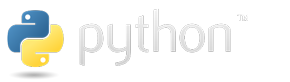
\includegraphics{index_files/mediabag/python-logo.png}

}

\caption{Python}

\end{figure}%

El control de flujo en Python se refiere a la forma en que se ejecutan
las instrucciones en un programa. Python proporciona varias estructuras
de control de flujo que permiten tomar decisiones, repetir tareas y
ejecutar instrucciones en función de ciertas condiciones.

La sintaxis de las estructuras de control de flujo en Python se basa en
la indentación, lo que significa que las instrucciones dentro de un
bloque de código deben estar indentadas con la misma cantidad de
espacios o tabulaciones. Esto hace que el código sea más legible y fácil
de entender.

En esta sección, aprenderemos sobre las siguientes estructuras de
control de flujo en Python:

\begin{itemize}
\tightlist
\item
  If y Condicionales
\item
  If, elif y else
\item
  And y Or
\item
  While loop
\item
  While, break y continue
\item
  For loop
\end{itemize}

\section{If y Condicionales}\label{if-y-condicionales}

Para entender el concepto de If y Condicionales en Python, primero
debemos comprender qué es una condición. Una condición es una expresión
que se evalúa como verdadera o falsa. En Python, las condiciones se
utilizan para tomar decisiones en un programa.

La estructura básica de un If en Python es la siguiente:

\begin{Shaded}
\begin{Highlighting}[]
\ControlFlowTok{if}\NormalTok{ condicion:}
    \CommentTok{\# Bloque de código si la condición es verdadera}
\end{Highlighting}
\end{Shaded}

En el código anterior, si la condición es verdadera, se ejecutará el
bloque de código dentro del If. Si la condición es falsa, el bloque de
código no se ejecutará.

Por ejemplo:

\begin{Shaded}
\begin{Highlighting}[]
\NormalTok{edad }\OperatorTok{=} \DecValTok{18}

\ControlFlowTok{if}\NormalTok{ edad }\OperatorTok{\textgreater{}=} \DecValTok{18}\NormalTok{:}
    \BuiltInTok{print}\NormalTok{(}\StringTok{"Eres mayor de edad"}\NormalTok{)}
\end{Highlighting}
\end{Shaded}

En el código anterior, si la variable \textbf{edad} es mayor o igual a
18, se imprimirá en la consola el mensaje ``Eres mayor de edad''.

\section{If, elif y else}\label{if-elif-y-else}

Además del If, Python también proporciona las palabras clave
\textbf{elif} y \textbf{else} para tomar decisiones más complejas en un
programa. La estructura básica de un If, elif y else en Python es la
siguiente:

\begin{Shaded}
\begin{Highlighting}[]
\ControlFlowTok{if}\NormalTok{ condicion1:}
    \CommentTok{\# Bloque de código si la condicion1 es verdadera}
\ControlFlowTok{elif}\NormalTok{ condicion2:}
    \CommentTok{\# Bloque de código si la condicion2 es verdadera}
\ControlFlowTok{else}\NormalTok{:}
    \CommentTok{\# Bloque de código si ninguna de las condiciones anteriores es verdadera}
\end{Highlighting}
\end{Shaded}

En el código anterior, si la \textbf{condicion1} es verdadera, se
ejecutará el bloque de código dentro del If. Si la \textbf{condicion1}
es falsa y la \textbf{condicion2} es verdadera, se ejecutará el bloque
de código dentro del \textbf{elif}. Si ninguna de las condiciones
anteriores es verdadera, se ejecutará el bloque de código dentro del
\textbf{else}.

Por ejemplo:

\begin{Shaded}
\begin{Highlighting}[]
\NormalTok{edad }\OperatorTok{=} \DecValTok{18}

\ControlFlowTok{if}\NormalTok{ edad }\OperatorTok{\textless{}} \DecValTok{18}\NormalTok{:}
    \BuiltInTok{print}\NormalTok{(}\StringTok{"Eres menor de edad"}\NormalTok{)}
\ControlFlowTok{elif}\NormalTok{ edad }\OperatorTok{==} \DecValTok{18}\NormalTok{:}
    \BuiltInTok{print}\NormalTok{(}\StringTok{"Tienes 18 años"}\NormalTok{)}
\ControlFlowTok{else}\NormalTok{:}
    \BuiltInTok{print}\NormalTok{(}\StringTok{"Eres mayor de edad"}\NormalTok{)}
\end{Highlighting}
\end{Shaded}

En el código anterior, si la variable \textbf{edad} es menor que 18, se
imprimirá en la consola el mensaje ``Eres menor de edad''. Si la
variable \textbf{edad} es igual a 18, se imprimirá en la consola el
mensaje ``Tienes 18 años''. Si ninguna de las condiciones anteriores es
verdadera, se imprimirá en la consola el mensaje ``Eres mayor de edad''.

\section{And y Or}\label{and-y-or}

Para entender el concepto de And y Or en Python, primero debemos
comprender cómo funcionan los operadores lógicos. Los operadores lógicos
se utilizan para combinar o modificar condiciones en una expresión
lógica.

En Python, los operadores lógicos más comunes son \textbf{and} y
\textbf{or}. El operador \textbf{and} devuelve \textbf{True} si ambas
condiciones son verdaderas. El operador \textbf{or} devuelve
\textbf{True} si al menos una de las condiciones es verdadera.

Por ejemplo:

\begin{Shaded}
\begin{Highlighting}[]
\NormalTok{edad }\OperatorTok{=} \DecValTok{18}

\ControlFlowTok{if}\NormalTok{ edad }\OperatorTok{\textgreater{}=} \DecValTok{18} \KeywordTok{and}\NormalTok{ edad }\OperatorTok{\textless{}=} \DecValTok{30}\NormalTok{:}
    \BuiltInTok{print}\NormalTok{(}\StringTok{"Tienes entre 18 y 30 años"}\NormalTok{)}
\end{Highlighting}
\end{Shaded}

En el código anterior, si la variable \textbf{edad} es mayor o igual a
18 y menor o igual a 30, se imprimirá en la consola el mensaje ``Tienes
entre 18 y 30 años''.

\section{While loop}\label{while-loop}

Para entender el concepto de While loop en Python, primero debemos
comprender qué es un bucle. Un bucle es una estructura de control que se
utiliza para repetir una secuencia de instrucciones varias veces. En
Python, el bucle \textbf{while} se utiliza para repetir un bloque de
código mientras una condición sea verdadera.

La estructura básica de un While loop en Python es la siguiente:

\begin{Shaded}
\begin{Highlighting}[]
\ControlFlowTok{while}\NormalTok{ condicion:}
    \CommentTok{\# Bloque de código que se repetirá mientras la condición sea verdadera}
\end{Highlighting}
\end{Shaded}

En el código anterior, si la condición es verdadera, se ejecutará el
bloque de código dentro del While loop. El bloque de código se repetirá
hasta que la condición sea falsa.

Por ejemplo:

\begin{Shaded}
\begin{Highlighting}[]
\NormalTok{contador }\OperatorTok{=} \DecValTok{0}

\ControlFlowTok{while}\NormalTok{ contador }\OperatorTok{\textless{}} \DecValTok{5}\NormalTok{:}
    \BuiltInTok{print}\NormalTok{(contador)}
\NormalTok{    contador }\OperatorTok{+=} \DecValTok{1}
\end{Highlighting}
\end{Shaded}

En el código anterior, se crea una variable \textbf{contador} con el
valor \textbf{0}. Luego, se ejecuta un While loop que imprime el valor
del \textbf{contador} y luego incrementa el \textbf{contador} en
\textbf{1} en cada iteración. El bucle se repetirá hasta que el
\textbf{contador} sea mayor o igual a \textbf{5}.

\section{While, break y continue}\label{while-break-y-continue}

Para entender el concepto de While, break y continue en Python, primero
debemos comprender cómo funcionan las palabras clave \textbf{break} y
\textbf{continue} en un bucle \textbf{while}.

La palabra clave \textbf{break} se utiliza para salir de un bucle
\textbf{while} antes de que la condición sea falsa. La palabra clave
\textbf{continue} se utiliza para saltar a la siguiente iteración del
bucle \textbf{while} sin ejecutar el resto del bloque de código.

Por ejemplo:

\begin{Shaded}
\begin{Highlighting}[]
\NormalTok{contador }\OperatorTok{=} \DecValTok{0}

\ControlFlowTok{while}\NormalTok{ contador }\OperatorTok{\textless{}} \DecValTok{5}\NormalTok{:}
    \ControlFlowTok{if}\NormalTok{ contador }\OperatorTok{==} \DecValTok{3}\NormalTok{:}
        \ControlFlowTok{break}
    \BuiltInTok{print}\NormalTok{(contador)}
\NormalTok{    contador }\OperatorTok{+=} \DecValTok{1}
\end{Highlighting}
\end{Shaded}

En el código anterior, se crea una variable \textbf{contador} con el
valor \textbf{0}. Luego, se ejecuta un While loop que imprime el valor
del \textbf{contador} y luego incrementa el \textbf{contador} en
\textbf{1} en cada iteración. Si el \textbf{contador} es igual a
\textbf{3}, se ejecuta la palabra clave \textbf{break} y se sale del
bucle.

\section{For loop}\label{for-loop}

Para entender el concepto de For loop en Python, primero debemos
comprender cómo funciona un bucle \textbf{for}. Un bucle \textbf{for} se
utiliza para iterar sobre una secuencia de elementos, como una lista,
una tupla, un diccionario, etc.

La estructura básica de un For loop en Python es la siguiente:

\begin{Shaded}
\begin{Highlighting}[]
\ControlFlowTok{for}\NormalTok{ elemento }\KeywordTok{in}\NormalTok{ secuencia:}
    \CommentTok{\# Bloque de código que se repetirá para cada elemento en la secuencia}
\end{Highlighting}
\end{Shaded}

En el código anterior, el bucle \textbf{for} recorre cada elemento en la
secuencia y ejecuta el bloque de código para cada elemento.

Por ejemplo:

\begin{Shaded}
\begin{Highlighting}[]
\NormalTok{numeros }\OperatorTok{=}\NormalTok{ [}\DecValTok{1}\NormalTok{, }\DecValTok{2}\NormalTok{, }\DecValTok{3}\NormalTok{, }\DecValTok{4}\NormalTok{, }\DecValTok{5}\NormalTok{]}

\ControlFlowTok{for}\NormalTok{ numero }\KeywordTok{in}\NormalTok{ numeros:}
    \BuiltInTok{print}\NormalTok{(numero)}
\end{Highlighting}
\end{Shaded}

En el código anterior, se crea una lista \textbf{numeros} con los
números del \textbf{1} al \textbf{5}. Luego, se ejecuta un For loop que
imprime cada número en la lista.

\chapter{Actividad}\label{actividad-2}

\section{instrucciones}\label{instrucciones-2}

\begin{enumerate}
\def\labelenumi{\arabic{enumi}.}
\item
  Crea una lista llamada \textbf{numeros} que contenga los números del
  \textbf{1} al \textbf{10}.
\item
  Crea una tupla llamada \textbf{colores} que contenga los colores
  \textbf{``rojo''}, \textbf{``verde''} y \textbf{``azul''}.
\item
  Crea un diccionario llamado \textbf{persona} que contenga las claves
  \textbf{``nombre''}, \textbf{``edad''} y \textbf{``ciudad''} con los
  valores \textbf{``Diego''}, \textbf{36} y \textbf{``Quito''}
  respectivamente.
\item
  Crea una variable booleana llamada \textbf{es\_mayor\_de\_edad} y
  asígnale el valor \textbf{True}.
\item
  Imprime en la consola las variables \textbf{numeros},
  \textbf{colores}, \textbf{persona} y \textbf{es\_mayor\_de\_edad}.
\item
  ¿Qué tipo de datos es la variable \textbf{numeros}? ¿Y la variable
  \textbf{colores}? ¿Y la variable \textbf{persona}? ¿Y la variable
  \textbf{es\_mayor\_de\_edad}?
\item
  ¿Qué tipo de datos es la variable \textbf{numeros{[}0{]}}? ¿Y la
  variable \textbf{colores{[}1{]}}? ¿Y la variable
  \textbf{persona{[}``nombre''{]}}? ¿Y la variable
  \textbf{es\_mayor\_de\_edad}?
\item
  ¿Qué tipo de datos es la variable \textbf{numeros{[}0:5{]}}? ¿Y la
  variable \textbf{colores{[}1:{]}}? ¿Y la variable
  \textbf{persona.keys()}? ¿Y la variable \textbf{es\_mayor\_de\_edad}?
\item
  ¿Qué tipo de datos es la variable \textbf{range(1, 10, 2)}? ¿Y la
  variable \textbf{range(10)}? ¿Y la variable \textbf{range(1, 10)}? ¿Y
  la variable \textbf{range(1, 10, 1)}?
\item
  ¿Qué tipo de datos es la variable \textbf{range(1, 10, 2){[}0{]}}? ¿Y
  la variable \textbf{range(10){[}0{]}}? ¿Y la variable \textbf{range(1,
  10){[}0{]}}? ¿Y la variable \textbf{range(1, 10, 1){[}0{]}}?
\end{enumerate}

Posibles soluciones

\begin{enumerate}
\def\labelenumi{\arabic{enumi}.}
\item
  La variable \textbf{numeros} es una lista.
\item
  La variable \textbf{colores} es una tupla.
\item
  La variable \textbf{persona} es un diccionario.
\item
  La variable \textbf{es\_mayor\_de\_edad} es un booleano.
\item
  La variable \textbf{numeros{[}0{]}} es un número.
\item
  La variable \textbf{colores{[}1{]}} es un String.
\item
  La variable \textbf{persona{[}``nombre''{]}} es un String.
\item
  La variable \textbf{numeros{[}0:5{]}} es una lista.
\item
  La variable \textbf{range(1, 10, 2)} es un objeto \textbf{range}.
\item
  La variable \textbf{range(1, 10, 2){[}0{]}} es un número.
\end{enumerate}

\chapter{Conclusiones}\label{conclusiones-2}

En esta sección, aprendimos sobre las estructuras de control de flujo en
Python, como If, elif, else, And, Or, While loop y For loop. Estas
estructuras nos permiten tomar decisiones, repetir tareas y ejecutar
instrucciones en función de ciertas condiciones en un programa. Es
importante comprender cómo funcionan estas estructuras para poder
escribir código más eficiente y legible en Python.

\chapter{Funciones y recursividad.}\label{funciones-y-recursividad.}

\begin{figure}[H]

{\centering 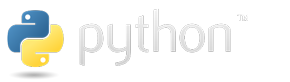
\includegraphics{index_files/mediabag/python-logo.png}

}

\caption{Python}

\end{figure}%

Las funciones son bloques de código reutilizables que realizan una tarea
específica. En Python, las funciones se definen utilizando la palabra
clave \textbf{def} seguida del nombre de la función y los parámetros
entre paréntesis. Por ejemplo:

\begin{Shaded}
\begin{Highlighting}[]
\KeywordTok{def}\NormalTok{ saludar():}
    \BuiltInTok{print}\NormalTok{(}\StringTok{"Hola, ¿cómo estás?"}\NormalTok{)}
\end{Highlighting}
\end{Shaded}

En el código anterior, se define una función llamada \textbf{saludar}
que imprime en la consola el mensaje ``Hola, ¿cómo estás?''. Para llamar
a una función en Python, simplemente se escribe el nombre de la función
seguido de paréntesis. Por ejemplo:

\begin{Shaded}
\begin{Highlighting}[]
\NormalTok{saludar()}
\end{Highlighting}
\end{Shaded}

En el código anterior, se llama a la función \textbf{saludar} y se
imprime en la consola el mensaje ``Hola, ¿cómo estás?''.

\section{Introducción a Funciones}\label{introducciuxf3n-a-funciones}

Para entender de mejor forma cómo funcionan las funciones en Python,
vamos a crear una función que reciba dos números como parámetros y
devuelva la suma de los mismos. Por ejemplo:

\begin{Shaded}
\begin{Highlighting}[]
\KeywordTok{def}\NormalTok{ sumar(a, b):}
    \ControlFlowTok{return}\NormalTok{ a }\OperatorTok{+}\NormalTok{ b}
\end{Highlighting}
\end{Shaded}

En el código anterior, se define una función llamada \textbf{sumar} que
recibe dos parámetros \textbf{a} y \textbf{b} y devuelve la suma de los
mismos. Para llamar a la función \textbf{sumar} y obtener el resultado,
se puede hacer de la siguiente manera:

\begin{Shaded}
\begin{Highlighting}[]
\NormalTok{resultado }\OperatorTok{=}\NormalTok{ sumar(}\DecValTok{5}\NormalTok{, }\DecValTok{3}\NormalTok{)}
\BuiltInTok{print}\NormalTok{(resultado)}
\end{Highlighting}
\end{Shaded}

En el código anterior, se llama a la función \textbf{sumar} con los
números \textbf{5} y \textbf{3} como parámetros y se imprime en la
consola el resultado \textbf{8}.

\section{Parámetros y Argumentos}\label{paruxe1metros-y-argumentos}

En Python, los parámetros son las variables que se definen en la
declaración de la función, mientras que los argumentos son los valores
que se pasan a la función cuando se llama. Por ejemplo:

\begin{Shaded}
\begin{Highlighting}[]
\KeywordTok{def}\NormalTok{ saludar(nombre):}
    \BuiltInTok{print}\NormalTok{(}\StringTok{"Hola, "} \OperatorTok{+}\NormalTok{ nombre }\OperatorTok{+} \StringTok{"!"}\NormalTok{)}
\end{Highlighting}
\end{Shaded}

En el código anterior, la función \textbf{saludar} tiene un parámetro
llamado \textbf{nombre}. Para llamar a la función \textbf{saludar} con
un argumento, se puede hacer de la siguiente manera:

\begin{Shaded}
\begin{Highlighting}[]
\NormalTok{saludar(}\StringTok{"Juan"}\NormalTok{)}
\end{Highlighting}
\end{Shaded}

En el código anterior, se llama a la función \textbf{saludar} con el
argumento \textbf{``Juan''} y se imprime en la consola el mensaje
``Hola, Juan!''.

\section{Retorno de valores}\label{retorno-de-valores}

En Python, las funciones pueden devolver valores utilizando la palabra
clave \textbf{return} seguida del valor que se desea devolver. Por
ejemplo:

\begin{Shaded}
\begin{Highlighting}[]
\KeywordTok{def}\NormalTok{ sumar(a, b):}
    \ControlFlowTok{return}\NormalTok{ a }\OperatorTok{+}\NormalTok{ b}
\end{Highlighting}
\end{Shaded}

En el código anterior, la función \textbf{sumar} devuelve la suma de los
números \textbf{a} y \textbf{b}. Para obtener el valor devuelto por la
función, se puede asignar a una variable y luego imprimir en la consola.
Por ejemplo:

\begin{Shaded}
\begin{Highlighting}[]
\NormalTok{resultado }\OperatorTok{=}\NormalTok{ sumar(}\DecValTok{5}\NormalTok{, }\DecValTok{3}\NormalTok{)}
\BuiltInTok{print}\NormalTok{(resultado)}
\end{Highlighting}
\end{Shaded}

En el código anterior, se llama a la función \textbf{sumar} con los
números \textbf{5} y \textbf{3} como parámetros, se asigna el resultado
a la variable \textbf{resultado} y se imprime en la consola el valor
\textbf{8}.

\section{Recursividad}\label{recursividad}

La recursividad es un concepto en programación en el que una función se
llama a sí misma para resolver un problema más pequeño. Por ejemplo, la
función factorial se puede definir de forma recursiva de la siguiente
manera:

\begin{Shaded}
\begin{Highlighting}[]
\KeywordTok{def}\NormalTok{ factorial(n):}
    \ControlFlowTok{if}\NormalTok{ n }\OperatorTok{==} \DecValTok{0}\NormalTok{:}
        \ControlFlowTok{return} \DecValTok{1}
    \ControlFlowTok{else}\NormalTok{:}
        \ControlFlowTok{return}\NormalTok{ n }\OperatorTok{*}\NormalTok{ factorial(n }\OperatorTok{{-}} \DecValTok{1}\NormalTok{)}
\end{Highlighting}
\end{Shaded}

En el código anterior, la función \textbf{factorial} calcula el
factorial de un número \textbf{n} de forma recursiva. Para llamar a la
función \textbf{factorial} y obtener el resultado, se puede hacer de la
siguiente manera:

\begin{Shaded}
\begin{Highlighting}[]
\NormalTok{resultado }\OperatorTok{=}\NormalTok{ factorial(}\DecValTok{5}\NormalTok{)}
\BuiltInTok{print}\NormalTok{(resultado)}
\end{Highlighting}
\end{Shaded}

En el código anterior, se llama a la función \textbf{factorial} con el
número \textbf{5} como parámetro y se imprime en la consola el resultado
\textbf{120}.

Otro ejemplo de recursividad es la función Fibonacci, que calcula el
enésimo término de la secuencia de Fibonacci de forma recursiva. Por
ejemplo:

\begin{Shaded}
\begin{Highlighting}[]
\KeywordTok{def}\NormalTok{ fibonacci(n):}
    \ControlFlowTok{if}\NormalTok{ n }\OperatorTok{\textless{}=} \DecValTok{1}\NormalTok{:}
        \ControlFlowTok{return}\NormalTok{ n}
    \ControlFlowTok{else}\NormalTok{:}
        \ControlFlowTok{return}\NormalTok{ fibonacci(n }\OperatorTok{{-}} \DecValTok{1}\NormalTok{) }\OperatorTok{+}\NormalTok{ fibonacci(n }\OperatorTok{{-}} \DecValTok{2}\NormalTok{)}
\end{Highlighting}
\end{Shaded}

En el código anterior, la función \textbf{fibonacci} calcula el enésimo
término de la secuencia de Fibonacci de forma recursiva. Para llamar a
la función \textbf{fibonacci} y obtener el resultado, se puede hacer de
la siguiente manera:

\begin{Shaded}
\begin{Highlighting}[]
\NormalTok{resultado }\OperatorTok{=}\NormalTok{ fibonacci(}\DecValTok{10}\NormalTok{)}
\BuiltInTok{print}\NormalTok{(resultado)}
\end{Highlighting}
\end{Shaded}

En el código anterior, se llama a la función \textbf{fibonacci} con el
número \textbf{10} como parámetro y se imprime en la consola el
resultado \textbf{55}.

\chapter{Actividad}\label{actividad-3}

\section{Instrucciones}\label{instrucciones-3}

\begin{enumerate}
\def\labelenumi{\arabic{enumi}.}
\item
  Crea una función llamada \textbf{saludar} que reciba un parámetro
  \textbf{nombre} y devuelva un saludo personalizado. Por ejemplo, si el
  nombre es \textbf{``Juan''}, la función debe devolver el mensaje
  \textbf{``Hola, Juan!''}.
\item
  Crea una función llamada \textbf{calcular\_promedio} que reciba una
  lista de números como parámetro y devuelva el promedio de los mismos.
  Por ejemplo, si la lista es \textbf{{[}1, 2, 3, 4, 5{]}}, la función
  debe devolver \textbf{3.0}.
\item
  Crea una función llamada \textbf{es\_par} que reciba un número como
  parámetro y devuelva \textbf{True} si el número es par y
  \textbf{False} si no lo es.
\item
  Crea una función llamada \textbf{calcular\_factorial} que reciba un
  número como parámetro y devuelva el factorial del mismo. Por ejemplo,
  si el número es \textbf{5}, la función debe devolver \textbf{120}.
\item
  Crea una función llamada \textbf{calcular\_fibonacci} que reciba un
  número como parámetro y devuelva el enésimo término de la secuencia de
  Fibonacci. Por ejemplo, si el número es \textbf{10}, la función debe
  devolver \textbf{55}.
\item
  Llama a cada una de las funciones creadas con valores de ejemplo y
  muestra los resultados en la consola.
\end{enumerate}

🔍 Pistas

\begin{itemize}
\tightlist
\item
  Para definir una función en Python, utiliza la palabra clave
  \textbf{def} seguida del nombre de la función y los parámetros entre
  paréntesis.

  \begin{itemize}
  \tightlist
  \item
    Para devolver un valor en una función, utiliza la palabra clave
    \textbf{return} seguida del valor que deseas devolver.
  \item
    Para llamar a una función en Python, simplemente escribe el nombre
    de la función seguido de paréntesis y los argumentos si es
    necesario.
  \end{itemize}
\end{itemize}

\chapter{Conclusiones}\label{conclusiones-3}

Las funciones y la recursividad son conceptos fundamentales en
programación que nos permiten escribir código más modular, reutilizable
y eficiente. Al entender cómo funcionan las funciones y cómo se pueden
llamar de forma recursiva, podemos resolver una amplia variedad de
problemas de programación de manera más sencilla y elegante. Además, las
funciones nos permiten encapsular la lógica de nuestro código y separar
las diferentes tareas en bloques más pequeños y manejables. En resumen,
las funciones y la recursividad son herramientas poderosas que nos
ayudan a escribir un código más limpio, organizado y fácil de mantener.

\part{Unidad 2: Programación Orientada a Objetos}

\chapter{Programacion Orientada a
Objetos.}\label{programacion-orientada-a-objetos.}

\begin{figure}[H]

{\centering 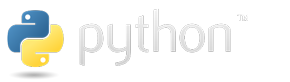
\includegraphics{index_files/mediabag/python-logo.png}

}

\caption{Python}

\end{figure}%

La Programación Orientada a Objetos (POO) es un paradigma de
programación que utiliza objetos y sus interacciones para diseñar
aplicaciones y programas de computadora. Está basado en varias técnicas,
incluyendo herencia, encapsulación, polimorfismo y abstracción.

Su sintaxis es más clara y sencilla de entender que otros paradigmas de
programación. Al permitirnos modelar entidades del mundo real de forma
más directa.

Ejemplo:

\begin{Shaded}
\begin{Highlighting}[]
\KeywordTok{class}\NormalTok{ Coche:}
    \KeywordTok{def} \FunctionTok{\_\_init\_\_}\NormalTok{(}\VariableTok{self}\NormalTok{, marca, modelo, color):}
        \VariableTok{self}\NormalTok{.marca }\OperatorTok{=}\NormalTok{ marca}
        \VariableTok{self}\NormalTok{.modelo }\OperatorTok{=}\NormalTok{ modelo}
        \VariableTok{self}\NormalTok{.color }\OperatorTok{=}\NormalTok{ color}

    \KeywordTok{def}\NormalTok{ acelerar(}\VariableTok{self}\NormalTok{):}
        \BuiltInTok{print}\NormalTok{(}\SpecialStringTok{f"El coche }\SpecialCharTok{\{}\VariableTok{self}\SpecialCharTok{.}\NormalTok{marca}\SpecialCharTok{\}}\SpecialStringTok{ }\SpecialCharTok{\{}\VariableTok{self}\SpecialCharTok{.}\NormalTok{modelo}\SpecialCharTok{\}}\SpecialStringTok{ de color }\SpecialCharTok{\{}\VariableTok{self}\SpecialCharTok{.}\NormalTok{color}\SpecialCharTok{\}}\SpecialStringTok{ está acelerando"}\NormalTok{)}

    \KeywordTok{def}\NormalTok{ frenar(}\VariableTok{self}\NormalTok{):}
        \BuiltInTok{print}\NormalTok{(}\SpecialStringTok{f"El coche }\SpecialCharTok{\{}\VariableTok{self}\SpecialCharTok{.}\NormalTok{marca}\SpecialCharTok{\}}\SpecialStringTok{ }\SpecialCharTok{\{}\VariableTok{self}\SpecialCharTok{.}\NormalTok{modelo}\SpecialCharTok{\}}\SpecialStringTok{ de color }\SpecialCharTok{\{}\VariableTok{self}\SpecialCharTok{.}\NormalTok{color}\SpecialCharTok{\}}\SpecialStringTok{ está frenando"}\NormalTok{)}

    \KeywordTok{def} \FunctionTok{\_\_str\_\_}\NormalTok{(}\VariableTok{self}\NormalTok{):}
        \ControlFlowTok{return} \SpecialStringTok{f"Coche }\SpecialCharTok{\{}\VariableTok{self}\SpecialCharTok{.}\NormalTok{marca}\SpecialCharTok{\}}\SpecialStringTok{ }\SpecialCharTok{\{}\VariableTok{self}\SpecialCharTok{.}\NormalTok{modelo}\SpecialCharTok{\}}\SpecialStringTok{ de color }\SpecialCharTok{\{}\VariableTok{self}\SpecialCharTok{.}\NormalTok{color}\SpecialCharTok{\}}\SpecialStringTok{"}
\end{Highlighting}
\end{Shaded}

En el código anterior se define una clase \textbf{Coche} con tres
atributos \textbf{marca}, \textbf{modelo} y \textbf{color}. Además, se
definen tres métodos \textbf{acelerar}, \textbf{frenar} y
\textbf{\textbf{str}}. El método \textbf{\textbf{str}} es un método
especial que se llama cuando se convierte un objeto a una cadena de
texto.

Para crear un objeto de la clase \textbf{Coche} se hace de la siguiente
manera:

\begin{Shaded}
\begin{Highlighting}[]
\NormalTok{coche }\OperatorTok{=}\NormalTok{ Coche(}\StringTok{"Toyota"}\NormalTok{, }\StringTok{"Corolla"}\NormalTok{, }\StringTok{"Rojo"}\NormalTok{)}
\BuiltInTok{print}\NormalTok{(coche)}
\NormalTok{coche.acelerar()}
\NormalTok{coche.frenar()}
\end{Highlighting}
\end{Shaded}

En el código anterior se crea un objeto \textbf{coche} de la clase
\textbf{Coche} con los atributos \textbf{Toyota}, \textbf{Corolla} y
\textbf{Rojo}. Luego se imprime el objeto \textbf{coche} y se llama a
los métodos \textbf{acelerar} y \textbf{frenar}.

\section{Objetos y Clases}\label{objetos-y-clases}

Los objetos son instancias de una clase. Una clase es una plantilla para
crear objetos. Los objetos tienen atributos y métodos.

\section{Atributos}\label{atributos}

Los atributos son variables que pertenecen a un objeto. Los atributos
pueden ser de cualquier tipo de datos.

Ejemplo:

\begin{Shaded}
\begin{Highlighting}[]
\KeywordTok{class}\NormalTok{ Coche:}
    \KeywordTok{def} \FunctionTok{\_\_init\_\_}\NormalTok{(}\VariableTok{self}\NormalTok{, marca, modelo, color):}
        \VariableTok{self}\NormalTok{.marca }\OperatorTok{=}\NormalTok{ marca}
        \VariableTok{self}\NormalTok{.modelo }\OperatorTok{=}\NormalTok{ modelo}
        \VariableTok{self}\NormalTok{.color }\OperatorTok{=}\NormalTok{ color}
\end{Highlighting}
\end{Shaded}

En el código anterior se definen tres atributos \textbf{marca},
\textbf{modelo} y \textbf{color}.

\section{Métodos}\label{muxe9todos}

Los métodos son funciones que pertenecen a un objeto. Los métodos pueden
acceder a los atributos de un objeto.

Ejemplo:

\begin{Shaded}
\begin{Highlighting}[]
\KeywordTok{class}\NormalTok{ Coche:}
    \KeywordTok{def}\NormalTok{ acelerar(}\VariableTok{self}\NormalTok{):}
        \BuiltInTok{print}\NormalTok{(}\SpecialStringTok{f"El coche }\SpecialCharTok{\{}\VariableTok{self}\SpecialCharTok{.}\NormalTok{marca}\SpecialCharTok{\}}\SpecialStringTok{ }\SpecialCharTok{\{}\VariableTok{self}\SpecialCharTok{.}\NormalTok{modelo}\SpecialCharTok{\}}\SpecialStringTok{ de color }\SpecialCharTok{\{}\VariableTok{self}\SpecialCharTok{.}\NormalTok{color}\SpecialCharTok{\}}\SpecialStringTok{ está acelerando"}\NormalTok{)}

    \KeywordTok{def}\NormalTok{ frenar(}\VariableTok{self}\NormalTok{):}
        \BuiltInTok{print}\NormalTok{(}\SpecialStringTok{f"El coche }\SpecialCharTok{\{}\VariableTok{self}\SpecialCharTok{.}\NormalTok{marca}\SpecialCharTok{\}}\SpecialStringTok{ }\SpecialCharTok{\{}\VariableTok{self}\SpecialCharTok{.}\NormalTok{modelo}\SpecialCharTok{\}}\SpecialStringTok{ de color }\SpecialCharTok{\{}\VariableTok{self}\SpecialCharTok{.}\NormalTok{color}\SpecialCharTok{\}}\SpecialStringTok{ está frenando"}\NormalTok{)}
\end{Highlighting}
\end{Shaded}

En el código anterior se definen dos métodos \textbf{acelerar} y
\textbf{frenar}.

\section{Self, Eliminar Propiedades y
Objetos}\label{self-eliminar-propiedades-y-objetos}

El primer parámetro de un método es \textbf{self}. \textbf{Self} es una
referencia al objeto actual. Se utiliza para acceder a los atributos y
métodos de un objeto.

Ejemplo:

\begin{Shaded}
\begin{Highlighting}[]
\KeywordTok{class}\NormalTok{ Coche:}
    \KeywordTok{def} \FunctionTok{\_\_init\_\_}\NormalTok{(}\VariableTok{self}\NormalTok{, marca, modelo, color):}
        \VariableTok{self}\NormalTok{.marca }\OperatorTok{=}\NormalTok{ marca}
        \VariableTok{self}\NormalTok{.modelo }\OperatorTok{=}\NormalTok{ modelo}
        \VariableTok{self}\NormalTok{.color }\OperatorTok{=}\NormalTok{ color}

    \KeywordTok{def}\NormalTok{ acelerar(}\VariableTok{self}\NormalTok{):}
        \BuiltInTok{print}\NormalTok{(}\SpecialStringTok{f"El coche }\SpecialCharTok{\{}\VariableTok{self}\SpecialCharTok{.}\NormalTok{marca}\SpecialCharTok{\}}\SpecialStringTok{ }\SpecialCharTok{\{}\VariableTok{self}\SpecialCharTok{.}\NormalTok{modelo}\SpecialCharTok{\}}\SpecialStringTok{ de color }\SpecialCharTok{\{}\VariableTok{self}\SpecialCharTok{.}\NormalTok{color}\SpecialCharTok{\}}\SpecialStringTok{ está acelerando"}\NormalTok{)}

    \KeywordTok{def}\NormalTok{ frenar(}\VariableTok{self}\NormalTok{):}
        \BuiltInTok{print}\NormalTok{(}\SpecialStringTok{f"El coche }\SpecialCharTok{\{}\VariableTok{self}\SpecialCharTok{.}\NormalTok{marca}\SpecialCharTok{\}}\SpecialStringTok{ }\SpecialCharTok{\{}\VariableTok{self}\SpecialCharTok{.}\NormalTok{modelo}\SpecialCharTok{\}}\SpecialStringTok{ de color }\SpecialCharTok{\{}\VariableTok{self}\SpecialCharTok{.}\NormalTok{color}\SpecialCharTok{\}}\SpecialStringTok{ está frenando"}\NormalTok{)}

    \KeywordTok{def} \FunctionTok{\_\_del\_\_}\NormalTok{(}\VariableTok{self}\NormalTok{):}
        \BuiltInTok{print}\NormalTok{(}\SpecialStringTok{f"El coche }\SpecialCharTok{\{}\VariableTok{self}\SpecialCharTok{.}\NormalTok{marca}\SpecialCharTok{\}}\SpecialStringTok{ }\SpecialCharTok{\{}\VariableTok{self}\SpecialCharTok{.}\NormalTok{modelo}\SpecialCharTok{\}}\SpecialStringTok{ de color }\SpecialCharTok{\{}\VariableTok{self}\SpecialCharTok{.}\NormalTok{color}\SpecialCharTok{\}}\SpecialStringTok{ ha sido eliminado"}\NormalTok{)}

\NormalTok{coche }\OperatorTok{=}\NormalTok{ Coche(}\StringTok{"Toyota"}\NormalTok{, }\StringTok{"Corolla"}\NormalTok{, }\StringTok{"Rojo"}\NormalTok{)}
\BuiltInTok{print}\NormalTok{(coche)}
\NormalTok{coche.acelerar()}
\NormalTok{coche.frenar()}
\KeywordTok{del}\NormalTok{ coche}
\end{Highlighting}
\end{Shaded}

En el código anterior se define un método especial \textbf{\textbf{del}}
que se llama cuando un objeto es eliminado.

\section{Herencia, Polimorfismo y
Encapsulación}\label{herencia-polimorfismo-y-encapsulaciuxf3n}

La herencia es una característica de la POO que permite crear una nueva
clase a partir de una clase existente. La nueva clase hereda los
atributos y métodos de la clase existente.

El polimorfismo es una característica de la POO que permite que un
objeto se computadora de diferentes maneras dependiendo del contexto.

La encapsulación es una característica de la POO que permite ocultar los
detalles de implementación de un objeto.

Ejemplo:

\begin{Shaded}
\begin{Highlighting}[]
\NormalTok{Class Deporte:}
    \KeywordTok{def} \FunctionTok{\_\_init\_\_}\NormalTok{(}\VariableTok{self}\NormalTok{, nombre):}
        \VariableTok{self}\NormalTok{.nombre }\OperatorTok{=}\NormalTok{ nombre}

    \KeywordTok{def}\NormalTok{ jugar(}\VariableTok{self}\NormalTok{):}
        \ControlFlowTok{pass}

\KeywordTok{class}\NormalTok{ Futbol(Deporte):}
  \KeywordTok{def}\NormalTok{ jugar(}\VariableTok{self}\NormalTok{):}
      \BuiltInTok{print}\NormalTok{(}\SpecialStringTok{f"Jugando futbol"}\NormalTok{)}

\KeywordTok{class}\NormalTok{ Baloncesto(Deporte):}
  \KeywordTok{def}\NormalTok{ jugar(}\VariableTok{self}\NormalTok{):}
      \BuiltInTok{print}\NormalTok{(}\SpecialStringTok{f"Jugando baloncesto"}\NormalTok{)}

\NormalTok{deporte }\OperatorTok{=}\NormalTok{ Futbol(}\StringTok{"Futbol"}\NormalTok{)}
\NormalTok{deporte.jugar()}

\NormalTok{deporte }\OperatorTok{=}\NormalTok{ Baloncesto(}\StringTok{"Baloncesto"}\NormalTok{)}
\NormalTok{deporte.jugar()}
\end{Highlighting}
\end{Shaded}

En el código anterior se define una clase \textbf{Deporte} con un método
\textbf{jugar}. Luego se definen dos clases \textbf{Futbol} y
\textbf{Baloncesto} que heredan de la clase \textbf{Deporte} y
sobrescriben el método \textbf{jugar}.

\section{Actividad}\label{actividad-4}

\begin{enumerate}
\def\labelenumi{\arabic{enumi}.}
\item
  Crear una clase \textbf{Persona} con los atributos \textbf{nombre},
  \textbf{edad} y \textbf{sexo}.
\item
  Crear una clase \textbf{Estudiante} que herede de la clase
  \textbf{Persona} con los atributos \textbf{carnet} y \textbf{carrera}.
\item
  Crear una clase \textbf{Profesor} que herede de la clase
  \textbf{Persona} con los atributos \textbf{codigo} y
  \textbf{especialidad}.
\item
  Crear una clase \textbf{Curso} con los atributos \textbf{nombre},
  \textbf{codigo} y \textbf{profesor}.
\item
  Crear una clase \textbf{Universidad} con los atributos \textbf{nombre}
  y \textbf{cursos}.
\item
  Crear un objeto \textbf{universidad} de la clase \textbf{Universidad}
  con el nombre \textbf{Universidad de El Salvador} y los siguientes
  cursos:
\end{enumerate}

\begin{itemize}
\tightlist
\item
  \textbf{Curso 1}: Nombre: \textbf{Matematicas}, Codigo:
  \textbf{MAT101}, Profesor: \textbf{Juan Perez}
\item
  \textbf{Curso 2}: Nombre: \textbf{Fisica}, Codigo: \textbf{FIS101},
  Profesor: \textbf{Maria Lopez}
\item
  \textbf{Curso 3}: Nombre: \textbf{Quimica}, Codigo: \textbf{QUI101},
  Profesor: \textbf{Pedro Ramirez}
\end{itemize}

\begin{enumerate}
\def\labelenumi{\arabic{enumi}.}
\setcounter{enumi}{6}
\item
  Imprimir el objeto \textbf{universidad}.
\item
  Crear un objeto \textbf{estudiante} de la clase \textbf{Estudiante}
  con los siguientes atributos:
\end{enumerate}

\begin{itemize}
\item
  Nombre: \textbf{Carlos Perez}
\item
  Edad: \textbf{20}
\item
  Sexo: \textbf{Masculino}
\item
  Carnet: \textbf{202010101}
\item
  Carrera: \textbf{Ingenieria en Sistemas Informaticos}
\end{itemize}

\begin{enumerate}
\def\labelenumi{\arabic{enumi}.}
\setcounter{enumi}{8}
\item
  Imprimir el objeto \textbf{estudiante}.
\item
  Crear un objeto \textbf{profesor} de la clase \textbf{Profesor} con
  los siguientes atributos:
\end{enumerate}

\begin{itemize}
\item
  Nombre: \textbf{Juan Perez}
\item
  Edad: \textbf{30}
\item
  Sexo: \textbf{Masculino}
\item
  Codigo: \textbf{202020202}
\item
  Especialidad: \textbf{Matematicas}
\end{itemize}

\begin{enumerate}
\def\labelenumi{\arabic{enumi}.}
\setcounter{enumi}{10}
\item
  Imprimir el objeto \textbf{profesor}.
\item
  Crear un objeto \textbf{curso} de la clase \textbf{Curso} con los
  siguientes atributos:
\end{enumerate}

\begin{itemize}
\item
  Nombre: \textbf{Matematicas}
\item
  Codigo: \textbf{MAT101}
\item
  Profesor: \textbf{Juan Perez}
\end{itemize}

\begin{enumerate}
\def\labelenumi{\arabic{enumi}.}
\setcounter{enumi}{12}
\item
  Imprimir el objeto \textbf{curso}.
\item
  Agregar el objeto \textbf{curso} al objeto \textbf{universidad}.
\item
  Imprimir el objeto \textbf{universidad}.
\item
  Crear un objeto \textbf{curso} de la clase \textbf{Curso} con los
  siguientes atributos:
\end{enumerate}

\begin{itemize}
\item
  Nombre: \textbf{Fisica}
\item
  Codigo: \textbf{FIS101}
\item
  Profesor: \textbf{Maria Lopez}
\end{itemize}

Respuesta

\begin{Shaded}
\begin{Highlighting}[]
\KeywordTok{class}\NormalTok{ Persona:}
    \KeywordTok{def} \FunctionTok{\_\_init\_\_}\NormalTok{(}\VariableTok{self}\NormalTok{, nombre, edad, sexo):}
        \VariableTok{self}\NormalTok{.nombre }\OperatorTok{=}\NormalTok{ nombre}
        \VariableTok{self}\NormalTok{.edad }\OperatorTok{=}\NormalTok{ edad}
        \VariableTok{self}\NormalTok{.sexo }\OperatorTok{=}\NormalTok{ sexo}

\KeywordTok{class}\NormalTok{ Estudiante(Persona):}
    \KeywordTok{def} \FunctionTok{\_\_init\_\_}\NormalTok{(}\VariableTok{self}\NormalTok{, nombre, edad, sexo, carnet, carrera):}
        \BuiltInTok{super}\NormalTok{().}\FunctionTok{\_\_init\_\_}\NormalTok{(nombre, edad, sexo)}
        \VariableTok{self}\NormalTok{.carnet }\OperatorTok{=}\NormalTok{ carnet}
        \VariableTok{self}\NormalTok{.carrera }\OperatorTok{=}\NormalTok{ carrera}

\KeywordTok{class}\NormalTok{ Profesor(Persona):}
    \KeywordTok{def} \FunctionTok{\_\_init\_\_}\NormalTok{(}\VariableTok{self}\NormalTok{, nombre, edad, sexo, codigo, especialidad):}
        \BuiltInTok{super}\NormalTok{().}\FunctionTok{\_\_init\_\_}\NormalTok{(nombre, edad, sexo)}
        \VariableTok{self}\NormalTok{.codigo }\OperatorTok{=}\NormalTok{ codigo}
        \VariableTok{self}\NormalTok{.especialidad }\OperatorTok{=}\NormalTok{ especialidad}

\KeywordTok{class}\NormalTok{ Curso:}
    \KeywordTok{def} \FunctionTok{\_\_init\_\_}\NormalTok{(}\VariableTok{self}\NormalTok{, nombre, codigo, profesor):}
        \VariableTok{self}\NormalTok{.nombre }\OperatorTok{=}\NormalTok{ nombre}
        \VariableTok{self}\NormalTok{.codigo }\OperatorTok{=}\NormalTok{ codigo}
        \VariableTok{self}\NormalTok{.profesor }\OperatorTok{=}\NormalTok{ profesor}

\KeywordTok{class}\NormalTok{ Universidad}
    \KeywordTok{def} \FunctionTok{\_\_init\_\_}\NormalTok{(}\VariableTok{self}\NormalTok{, nombre):}
        \VariableTok{self}\NormalTok{.nombre }\OperatorTok{=}\NormalTok{ nombre}
        \VariableTok{self}\NormalTok{.cursos }\OperatorTok{=}\NormalTok{ []}

\NormalTok{universidad }\OperatorTok{=}\NormalTok{ Universidad(}\StringTok{"Universidad de las Fuerzas Armadas ESPE"}\NormalTok{)}
\NormalTok{curso1 }\OperatorTok{=}\NormalTok{ Curso(}\StringTok{"Matematicas"}\NormalTok{, }\StringTok{"MAT101"}\NormalTok{, }\StringTok{"Juan Perez"}\NormalTok{)}
\NormalTok{curso2 }\OperatorTok{=}\NormalTok{ Curso(}\StringTok{"Fisica"}\NormalTok{, }\StringTok{"FIS101"}\NormalTok{, }\StringTok{"Maria Lopez"}\NormalTok{)}
\NormalTok{curso3 }\OperatorTok{=}\NormalTok{ Curso(}\StringTok{"Quimica"}\NormalTok{, }\StringTok{"QUI101"}\NormalTok{, }\StringTok{"Pedro Ramirez"}\NormalTok{)}
\NormalTok{universidad.cursos.append(curso1)}
\NormalTok{universidad.cursos.append(curso2)}
\NormalTok{universidad.cursos.append(curso3)}
\BuiltInTok{print}\NormalTok{(universidad)}

\NormalTok{estudiante }\OperatorTok{=}\NormalTok{ Estudiante(}\StringTok{"Carlos Perez"}\NormalTok{, }\DecValTok{20}\NormalTok{, }\StringTok{"Masculino"}\NormalTok{, }\StringTok{"202010101"}\NormalTok{, }\StringTok{"Ingenieria en Sistemas Informaticos"}\NormalTok{)}
\BuiltInTok{print}\NormalTok{(estudiante)}

\NormalTok{profesor }\OperatorTok{=}\NormalTok{ Profesor(}\StringTok{"Juan Perez"}\NormalTok{, }\DecValTok{30}\NormalTok{, }\StringTok{"Masculino"}\NormalTok{, }\StringTok{"202020202"}\NormalTok{, }\StringTok{"Matematicas"}\NormalTok{)}
\BuiltInTok{print}\NormalTok{(profesor)}

\NormalTok{curso }\OperatorTok{=}\NormalTok{ Curso(}\StringTok{"Matematicas"}\NormalTok{, }\StringTok{"MAT101"}\NormalTok{, }\StringTok{"Juan Perez"}\NormalTok{)}
\BuiltInTok{print}\NormalTok{(curso)}

\NormalTok{curso }\OperatorTok{=}\NormalTok{ Curso(}\StringTok{"Fisica"}\NormalTok{, }\StringTok{"FIS101"}\NormalTok{, }\StringTok{"Maria Lopez"}\NormalTok{)}
\NormalTok{universidad.cursos.append(curso)}
\BuiltInTok{print}\NormalTok{(universidad)}
\end{Highlighting}
\end{Shaded}

\chapter{Conclusiones}\label{conclusiones-4}

La Programación Orientada a Objetos (POO) es un paradigma de
programación que utiliza objetos y sus interacciones para diseñar
aplicaciones y programas de computadora. Está basado en varias técnicas,
incluyendo herencia, encapsulación, polimorfismo y abstracción.

\part{Unidad 3: Módulos y Paquetes}

\chapter{Módulos en Python}\label{muxf3dulos-en-python}

\begin{figure}[H]

{\centering 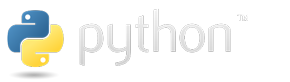
\includegraphics{index_files/mediabag/python-logo.png}

}

\caption{Python}

\end{figure}%

\section{Introducción a Módulos.}\label{introducciuxf3n-a-muxf3dulos.}

Los módulos en python son archivos que contienen definiciones y
declaraciones de python. Los módulos permiten organizar el código en
archivos separados. Los módulos se utilizan para reutilizar código y
para mantener el código organizado.

Ejemplo:

\begin{Shaded}
\begin{Highlighting}[]
\CommentTok{\# modulo.py }
\KeywordTok{def}\NormalTok{ saludar():}
    \BuiltInTok{print}\NormalTok{(}\StringTok{"Hola Mundo"}\NormalTok{)}
\end{Highlighting}
\end{Shaded}

En el código anterior se define un módulo \textbf{modulo.py} que
contiene una función \textbf{saludar}.

Ejemplo:

\begin{Shaded}
\begin{Highlighting}[]
\CommentTok{\# modulo.py}
\KeywordTok{def}\NormalTok{ despedir():}
    \BuiltInTok{print}\NormalTok{(}\StringTok{"Adiós Mundo"}\NormalTok{)}
\end{Highlighting}
\end{Shaded}

En el código anterior se define un módulo \textbf{modulo.py} que
contiene una función \textbf{despedir}.

\section{Creando el primer Módulo.}\label{creando-el-primer-muxf3dulo.}

Para crear nuestro primer módulo en python, creamos un archivo con
extensión \textbf{.py} y definimos las funciones que queremos exportar.

Ejemplo:

\begin{Shaded}
\begin{Highlighting}[]
\CommentTok{\# modulo\_saludar.py}

\KeywordTok{def}\NormalTok{ saludar(nombre):}
    \BuiltInTok{print}\NormalTok{(}\SpecialStringTok{f"Hola }\SpecialCharTok{\{}\NormalTok{nombre}\SpecialCharTok{\}}\SpecialStringTok{"}\NormalTok{)}
\end{Highlighting}
\end{Shaded}

En el código anterior se define un módulo \textbf{modulo\_saludar.py}
que contiene una función \textbf{saludar}.

\section{Creando el segundo
Módulo.}\label{creando-el-segundo-muxf3dulo.}

Para crear nuestro segundo módulo en python, creamos un archivo con
extensión \textbf{.py} y definimos las funciones que queremos exportar.

Ejemplo:

\begin{Shaded}
\begin{Highlighting}[]
\CommentTok{\# modulo\_despedir.py}

\KeywordTok{def}\NormalTok{ despedir(nombre):}
    \BuiltInTok{print}\NormalTok{(}\SpecialStringTok{f"Adiós }\SpecialCharTok{\{}\NormalTok{nombre}\SpecialCharTok{\}}\SpecialStringTok{"}\NormalTok{)}
\end{Highlighting}
\end{Shaded}

En el código anterior se define un módulo \textbf{modulo\_despedir.py}
que contiene una función \textbf{despedir}.

\section{Creando el archivo
principal.}\label{creando-el-archivo-principal.}

Para utilizar los módulos en python, creamos un archivo principal con
extensión \textbf{.py} e importamos los módulos que queremos utilizar.

Ejemplo:

\begin{Shaded}
\begin{Highlighting}[]
\CommentTok{\# main.py}
\ImportTok{import}\NormalTok{ modulo\_saludar}
\ImportTok{import}\NormalTok{ modulo\_despedir}

\VariableTok{\_\_name\_\_} \OperatorTok{==} \StringTok{"\_\_main\_\_"}
\NormalTok{modulo\_saludar.saludar(}\StringTok{"Juan"}\NormalTok{)}
\NormalTok{modulo\_despedir.despedir(}\StringTok{"Juan"}\NormalTok{)}
\end{Highlighting}
\end{Shaded}

En el código anterior se importan los módulos \textbf{modulo\_saludar} y
\textbf{modulo\_despedir} y se utilizan las funciones \textbf{saludar} y
\textbf{despedir}.

\section{Importando Módulos.}\label{importando-muxf3dulos.}

Para importar un módulo en python se utiliza la palabra clave
\textbf{import} seguida del nombre del módulo.

\begin{tcolorbox}[enhanced jigsaw, bottomrule=.15mm, rightrule=.15mm, colframe=quarto-callout-tip-color-frame, arc=.35mm, breakable, colbacktitle=quarto-callout-tip-color!10!white, toptitle=1mm, colback=white, opacitybacktitle=0.6, opacityback=0, bottomtitle=1mm, toprule=.15mm, titlerule=0mm, left=2mm, coltitle=black, leftrule=.75mm, title=\textcolor{quarto-callout-tip-color}{\faLightbulb}\hspace{0.5em}{Tip}]

Utilizaremos el mismo ejemplo anterior.

\end{tcolorbox}

Ejemplo:

\begin{Shaded}
\begin{Highlighting}[]
\CommentTok{\# main.py}

\ImportTok{import}\NormalTok{ modulo\_saludar}
\ImportTok{import}\NormalTok{ modulo\_despedir}

\NormalTok{modulo\_saludar.saludar(}\StringTok{"Juan"}\NormalTok{)}
\NormalTok{modulo\_despedir.despedir(}\StringTok{"Juan"}\NormalTok{)}
\end{Highlighting}
\end{Shaded}

En el código anterior se importan los módulos \textbf{modulo\_saludar} y
\textbf{modulo\_despedir} y se utilizan las funciones \textbf{saludar} y
\textbf{despedir}.

\section{Renombrando Módulos.}\label{renombrando-muxf3dulos.}

Para renombrar un módulo en python se utiliza la palabra clave
\textbf{as} seguida del nuevo nombre.

Ejemplo:

\begin{Shaded}
\begin{Highlighting}[]
\CommentTok{\# main.py}

\ImportTok{import}\NormalTok{ modulo\_saludar }\ImportTok{as}\NormalTok{ saludar}
\ImportTok{import}\NormalTok{ modulo\_despedir }\ImportTok{as}\NormalTok{ despedir}

\NormalTok{saludar.saludar(}\StringTok{"Juan"}\NormalTok{)}
\NormalTok{despedir.despedir(}\StringTok{"Juan"}\NormalTok{)}
\end{Highlighting}
\end{Shaded}

En el código anterior se importan los módulos \textbf{modulo\_saludar} y
\textbf{modulo\_despedir} con los nombres \textbf{saludar} y
\textbf{despedir} respectivamente.

\section{Seleccionando Elementos}\label{seleccionando-elementos}

Para importar elementos específicos de un módulo en python se utiliza la
palabra clave \textbf{from} seguida del nombre del módulo y la palabra
clave \textbf{import} seguida del nombre del elemento.

Ejemplo:

\begin{Shaded}
\begin{Highlighting}[]
\CommentTok{\# main.py}

\ImportTok{from}\NormalTok{ modulo\_saludar }\ImportTok{import}\NormalTok{ saludar}

\NormalTok{saludar(}\StringTok{"Juan"}\NormalTok{)}

\ImportTok{from}\NormalTok{ modulo\_despedir }\ImportTok{import}\NormalTok{ despedir}

\NormalTok{despedir(}\StringTok{"Juan"}\NormalTok{)}
\end{Highlighting}
\end{Shaded}

En el código anterior se importan las funciones \textbf{saludar} y
\textbf{despedir} del módulo \textbf{modulo\_saludar} y
\textbf{modulo\_despedir} respectivamente.

\section{Seleccionando lo importado y
pip}\label{seleccionando-lo-importado-y-pip}

Vamos a crear una aplicación divertida con emojis.

Ejemplo:

\begin{Shaded}
\begin{Highlighting}[]
\CommentTok{\# modulo\_emojis.py}

\KeywordTok{def}\NormalTok{ sonreir():}
    \BuiltInTok{print}\NormalTok{(}\StringTok{"😊"}\NormalTok{)}

\KeywordTok{def}\NormalTok{ llorar():}
    \BuiltInTok{print}\NormalTok{(}\StringTok{"😢"}\NormalTok{)}

\CommentTok{\# main.py}

\ImportTok{from}\NormalTok{ modulo\_emojis }\ImportTok{import}\NormalTok{ sonreir}

\NormalTok{sonreir()}

\ImportTok{from}\NormalTok{ modulo\_emojis }\ImportTok{import}\NormalTok{ llorar}

\NormalTok{llorar()}
\end{Highlighting}
\end{Shaded}

En el código anterior se definen dos funciones \textbf{sonreir} y
\textbf{llorar} en el módulo \textbf{modulo\_emojis}. En el archivo
\textbf{main.py} se importan las funciones \textbf{sonreir} y
\textbf{llorar} y se utilizan.

\section{Instalando Módulos con
pip}\label{instalando-muxf3dulos-con-pip}

Para instalar módulos en python se utiliza la herramienta \textbf{pip}.
\textbf{pip} es un sistema de gestión de paquetes utilizado para
instalar y administrar paquetes de software escritos en python.

Ejemplo:

\begin{Shaded}
\begin{Highlighting}[]
\ExtensionTok{pip}\NormalTok{ install numpy}
\end{Highlighting}
\end{Shaded}

En el código anterior se instala el módulo \textbf{numpy} utilizando
\textbf{pip}.

Ahora pra utilizar este módulo en nuestro código, simplemente lo
importamos.

Ejemplo:

\begin{Shaded}
\begin{Highlighting}[]
\ImportTok{import}\NormalTok{ numpy }\ImportTok{as}\NormalTok{ np}

\NormalTok{a }\OperatorTok{=}\NormalTok{ np.array([}\DecValTok{1}\NormalTok{, }\DecValTok{2}\NormalTok{, }\DecValTok{3}\NormalTok{, }\DecValTok{4}\NormalTok{, }\DecValTok{5}\NormalTok{])}

\BuiltInTok{print}\NormalTok{(a)}
\end{Highlighting}
\end{Shaded}

\section{Actividad}\label{actividad-5}

\begin{enumerate}
\def\labelenumi{\arabic{enumi}.}
\item
  Crear un módulo \textbf{modulo\_calculadora.py} que contenga las
  funciones \textbf{sumar}, \textbf{restar}, \textbf{multiplicar} y
  \textbf{dividir}.
\item
  Crear un archivo \textbf{main.py} que importe el módulo
  \textbf{modulo\_calculadora} y utilice las funciones \textbf{sumar},
  \textbf{restar}, \textbf{multiplicar} y \textbf{dividir}.
\item
  Ejecutar el archivo \textbf{main.py}.
\item
  Instalar el módulo \textbf{numpy} utilizando \textbf{pip}.
\item
  Crear un archivo \textbf{main\_numpy.py} que importe el módulo
  \textbf{numpy} y utilice la función \textbf{array} para crear un
  arreglo de números.
\item
  Ejecutar el archivo \textbf{main\_numpy.py}.
\item
  Crear un archivo \textbf{main\_pandas.py} que importe el módulo
  \textbf{pandas} y utilice la función \textbf{DataFrame} para crear un
  DataFrame.
\item
  Ejecutar el archivo \textbf{main\_pandas.py}.
\item
  Crear un archivo \textbf{main\_matplotlib.py} que importe el módulo
  \textbf{matplotlib} y utilice la función \textbf{plot} para graficar
  una función.
\item
  Ejecutar el archivo \textbf{main\_matplotlib.py}.
\end{enumerate}

Respuesta

\begin{enumerate}
\def\labelenumi{\arabic{enumi}.}
\tightlist
\item
  Crear un módulo \textbf{modulo\_calculadora.py} que contenga las
  funciones \textbf{sumar}, \textbf{restar}, \textbf{multiplicar} y
  \textbf{dividir}.
\end{enumerate}

\begin{Shaded}
\begin{Highlighting}[]
\CommentTok{\# modulo\_calculadora.py}

\KeywordTok{def}\NormalTok{ sumar(a, b):}
    \ControlFlowTok{return}\NormalTok{ a }\OperatorTok{+}\NormalTok{ b}

\KeywordTok{def}\NormalTok{ restar(a, b):}
    \ControlFlowTok{return}\NormalTok{ a }\OperatorTok{{-}}\NormalTok{ b}

\KeywordTok{def}\NormalTok{ multiplicar(a, b):}
    \ControlFlowTok{return}\NormalTok{ a }\OperatorTok{*}\NormalTok{ b}

\KeywordTok{def}\NormalTok{ dividir(a, b):}
    \ControlFlowTok{return}\NormalTok{ a }\OperatorTok{/}\NormalTok{ b}
\end{Highlighting}
\end{Shaded}

En el código anterior se define un módulo
\textbf{modulo\_calculadora.py} que contiene las funciones
\textbf{sumar}, \textbf{restar}, \textbf{multiplicar} y
\textbf{dividir}.

\begin{enumerate}
\def\labelenumi{\arabic{enumi}.}
\setcounter{enumi}{1}
\tightlist
\item
  Crear un archivo \textbf{main.py} que importe el módulo
  \textbf{modulo\_calculadora} y utilice las funciones \textbf{sumar},
  \textbf{restar}, \textbf{multiplicar} y \textbf{dividir}.
\end{enumerate}

\begin{Shaded}
\begin{Highlighting}[]
\CommentTok{\# main.py}

\ImportTok{import}\NormalTok{ modulo\_calculadora}

\BuiltInTok{print}\NormalTok{(modulo\_calculadora.sumar(}\DecValTok{2}\NormalTok{, }\DecValTok{3}\NormalTok{))}
\BuiltInTok{print}\NormalTok{(modulo\_calculadora.restar(}\DecValTok{5}\NormalTok{, }\DecValTok{3}\NormalTok{))}
\BuiltInTok{print}\NormalTok{(modulo\_calculadora.multiplicar(}\DecValTok{2}\NormalTok{, }\DecValTok{3}\NormalTok{))}
\BuiltInTok{print}\NormalTok{(modulo\_calculadora.dividir(}\DecValTok{6}\NormalTok{, }\DecValTok{3}\NormalTok{))}
\end{Highlighting}
\end{Shaded}

En el código anterior se importa el módulo \textbf{modulo\_calculadora}
y se utilizan las funciones \textbf{sumar}, \textbf{restar},
\textbf{multiplicar} y \textbf{dividir}.

\begin{enumerate}
\def\labelenumi{\arabic{enumi}.}
\setcounter{enumi}{2}
\tightlist
\item
  Ejecutar el archivo \textbf{main.py}.
\end{enumerate}

\begin{Shaded}
\begin{Highlighting}[]
\ExtensionTok{python}\NormalTok{ main.py}
\end{Highlighting}
\end{Shaded}

El resultado es:

\begin{Shaded}
\begin{Highlighting}[]
\ExtensionTok{5}
\ExtensionTok{2}
\ExtensionTok{6}
\ExtensionTok{2.0}
\end{Highlighting}
\end{Shaded}

\begin{enumerate}
\def\labelenumi{\arabic{enumi}.}
\setcounter{enumi}{3}
\tightlist
\item
  Instalar el módulo \textbf{numpy} utilizando \textbf{pip}.
\end{enumerate}

\begin{Shaded}
\begin{Highlighting}[]
\ExtensionTok{pip}\NormalTok{ install numpy}
\end{Highlighting}
\end{Shaded}

\begin{enumerate}
\def\labelenumi{\arabic{enumi}.}
\setcounter{enumi}{4}
\tightlist
\item
  Crear un archivo \textbf{main\_numpy.py} que importe el módulo
  \textbf{numpy} y utilice la función \textbf{array} para crear un
  arreglo de números.
\end{enumerate}

\begin{Shaded}
\begin{Highlighting}[]

\CommentTok{\# main\_numpy.py}

\ImportTok{import}\NormalTok{ numpy }\ImportTok{as}\NormalTok{ np}

\NormalTok{a }\OperatorTok{=}\NormalTok{ np.array([}\DecValTok{1}\NormalTok{, }\DecValTok{2}\NormalTok{, }\DecValTok{3}\NormalTok{, }\DecValTok{4}\NormalTok{, }\DecValTok{5}\NormalTok{])}

\BuiltInTok{print}\NormalTok{(a)}
\end{Highlighting}
\end{Shaded}

En el código anterior se importa el módulo \textbf{numpy} y se utiliza
la función \textbf{array} para crear un arreglo de números.

\begin{enumerate}
\def\labelenumi{\arabic{enumi}.}
\setcounter{enumi}{5}
\tightlist
\item
  Ejecutar el archivo \textbf{main\_numpy.py}.
\end{enumerate}

\begin{Shaded}
\begin{Highlighting}[]
\ExtensionTok{python}\NormalTok{ main\_numpy.py}
\end{Highlighting}
\end{Shaded}

\begin{enumerate}
\def\labelenumi{\arabic{enumi}.}
\setcounter{enumi}{6}
\tightlist
\item
  Crear un archivo \textbf{main\_pandas.py} que importe el módulo
  \textbf{pandas} y utilice la función \textbf{DataFrame} para crear un
  DataFrame.
\end{enumerate}

\begin{Shaded}
\begin{Highlighting}[]
\CommentTok{\# main\_pandas.py}

\ImportTok{import}\NormalTok{ pandas }\ImportTok{as}\NormalTok{ pd}

\NormalTok{data }\OperatorTok{=}\NormalTok{ \{}
    \StringTok{\textquotesingle{}Nombre\textquotesingle{}}\NormalTok{: [}\StringTok{\textquotesingle{}Juan\textquotesingle{}}\NormalTok{, }\StringTok{\textquotesingle{}Maria\textquotesingle{}}\NormalTok{, }\StringTok{\textquotesingle{}Pedro\textquotesingle{}}\NormalTok{],}
    \StringTok{\textquotesingle{}Edad\textquotesingle{}}\NormalTok{: [}\DecValTok{20}\NormalTok{, }\DecValTok{25}\NormalTok{, }\DecValTok{30}\NormalTok{]}
\NormalTok{\}}

\NormalTok{df }\OperatorTok{=}\NormalTok{ pd.DataFrame(data)}

\BuiltInTok{print}\NormalTok{(df)}
\end{Highlighting}
\end{Shaded}

En el código anterior se importa el módulo \textbf{pandas} y se utiliza
la función \textbf{DataFrame} para crear un DataFrame.

\begin{enumerate}
\def\labelenumi{\arabic{enumi}.}
\setcounter{enumi}{7}
\tightlist
\item
  Ejecutar el archivo \textbf{main\_pandas.py}.
\end{enumerate}

\begin{Shaded}
\begin{Highlighting}[]
\ExtensionTok{python}\NormalTok{ main\_pandas.py}
\end{Highlighting}
\end{Shaded}

\begin{enumerate}
\def\labelenumi{\arabic{enumi}.}
\setcounter{enumi}{8}
\tightlist
\item
  Crear un archivo \textbf{main\_matplotlib.py} que importe el módulo
  \textbf{matplotlib} y utilice la función \textbf{plot} para graficar
  una función.
\end{enumerate}

\begin{Shaded}
\begin{Highlighting}[]
\CommentTok{\# main\_matplotlib.py}

\ImportTok{import}\NormalTok{ matplotlib.pyplot }\ImportTok{as}\NormalTok{ plt}
\ImportTok{import}\NormalTok{ numpy }\ImportTok{as}\NormalTok{ np}

\NormalTok{x }\OperatorTok{=}\NormalTok{ np.linspace(}\DecValTok{0}\NormalTok{, }\DecValTok{10}\NormalTok{, }\DecValTok{100}\NormalTok{)}

\NormalTok{y }\OperatorTok{=}\NormalTok{ np.sin(x)}

\NormalTok{plt.plot(x, y)}

\NormalTok{plt.show()}
\end{Highlighting}
\end{Shaded}

En el código anterior se importa el módulo \textbf{matplotlib} y se
utiliza la función \textbf{plot} para graficar una función.

\begin{enumerate}
\def\labelenumi{\arabic{enumi}.}
\setcounter{enumi}{9}
\tightlist
\item
  Ejecutar el archivo \textbf{main\_matplotlib.py}.
\end{enumerate}

\begin{Shaded}
\begin{Highlighting}[]
\ExtensionTok{python}\NormalTok{ main\_matplotlib.py}
\end{Highlighting}
\end{Shaded}

\chapter{Conclusiones}\label{conclusiones-5}

Los módulos en python son archivos que contienen definiciones y
declaraciones de python. Los módulos permiten organizar el código en
archivos separados. Los módulos se utilizan para reutilizar código y
para mantener el código organizado.

\part{Proyectos}

\chapter{🪤✏️ Laboratorio: Construcción de un Juego de Ahorcado en
Python}\label{laboratorio-construcciuxf3n-de-un-juego-de-ahorcado-en-python}

\begin{figure}[H]

{\centering 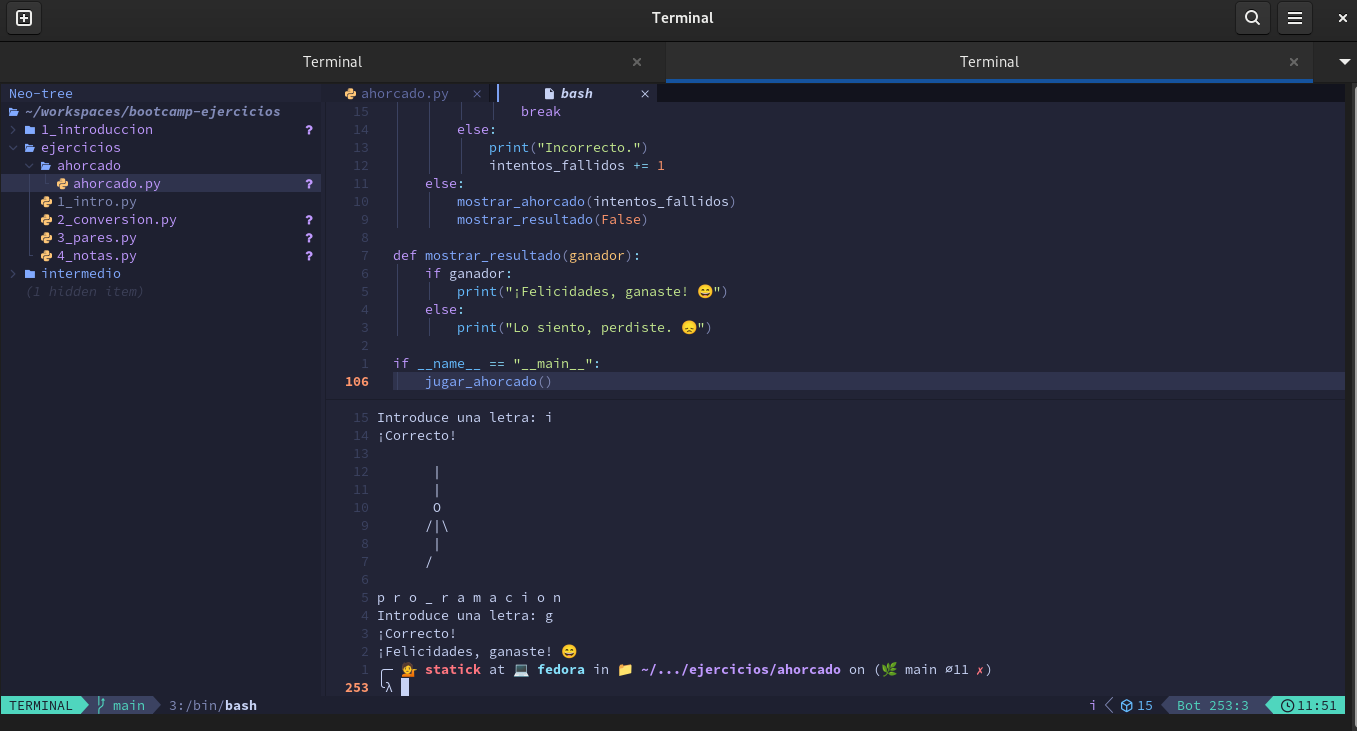
\includegraphics{unidades/Proyectos/images/ahorcado.png}

}

\caption{Ahorcado}

\end{figure}%

\section{Objetivos del Laboratorio}\label{objetivos-del-laboratorio}

\begin{enumerate}
\def\labelenumi{\arabic{enumi}.}
\tightlist
\item
  Desarrollar un juego de Ahorcado usando funciones en Python.
\item
  Usar estructuras de datos como listas y cadenas de texto.
\item
  Implementar lógica condicional y bucles para manejar el flujo del
  juego.
\item
  Mostrar mensajes finales (con emojis) según el resultado del juego.
\end{enumerate}

\section{Prerrequisitos}\label{prerrequisitos}

\begin{itemize}
\item
  \textbf{Conocimiento básico de Python:} funciones, listas, cadenas,
  condicionales y bucles.
\item
  Instalación de Python 3 en tu equipo.
\end{itemize}

\section{Paso 1: Crear la Estructura Inicial del
Proyecto}\label{paso-1-crear-la-estructura-inicial-del-proyecto}

\subsection{Crear un archivo de
Python:}\label{crear-un-archivo-de-python}

Abre tu editor de texto o IDE favorito (se recomienda utilizar Vscode) y
crea un nuevo archivo llamado \textbf{ahorcado.py}.

\textbf{Definir el objetivo del proyecto en el archivo:}

Añade un comentario en la primera línea que describa el propósito del
proyecto:

\begin{Shaded}
\begin{Highlighting}[]
\CommentTok{\# Juego de Ahorcado en Python}
\end{Highlighting}
\end{Shaded}

\section{Paso 2: Definir las Etapas del Ahorcado en
ASCII}\label{paso-2-definir-las-etapas-del-ahorcado-en-ascii}

\subsection{Crear la lista
AHORCADO\_DIBUJO:}\label{crear-la-lista-ahorcado_dibujo}

Define las etapas progresivas del dibujo del ahorcado usando una lista
de cadenas en ASCII.

Cada elemento de la lista representa una etapa del juego.

\begin{Shaded}
\begin{Highlighting}[]
\NormalTok{AHORCADO\_DIBUJO }\OperatorTok{=}\NormalTok{ [}
    \StringTok{"""}
\StringTok{       |}
\StringTok{       |}
\StringTok{       |}
\StringTok{       |}
\StringTok{    """}\NormalTok{,}
    \StringTok{"""}
\StringTok{       |}
\StringTok{       |}
\StringTok{       O}
\StringTok{       |}
\StringTok{    """}\NormalTok{,}
    \StringTok{"""}
\StringTok{       |}
\StringTok{       |}
\StringTok{       O}
\StringTok{      /|}
\StringTok{    """}\NormalTok{,}
    \StringTok{"""}
\StringTok{       |}
\StringTok{       |}
\StringTok{       O}
\StringTok{      /|}\CharTok{\textbackslash{}\textbackslash{}}
\StringTok{       |}
\StringTok{    """}\NormalTok{,}
    \StringTok{"""}
\StringTok{       |}
\StringTok{       |}
\StringTok{       O}
\StringTok{      /|}\CharTok{\textbackslash{}\textbackslash{}}
\StringTok{       |}
\StringTok{      /}
\StringTok{    """}\NormalTok{,}
    \StringTok{"""}
\StringTok{       |}
\StringTok{       |}
\StringTok{       O}
\StringTok{      /|}\CharTok{\textbackslash{}\textbackslash{}}
\StringTok{       |}
\StringTok{      / }\CharTok{\textbackslash{}\textbackslash{}}
\StringTok{    """}
\NormalTok{]}
\end{Highlighting}
\end{Shaded}

\subsection{Prueba del dibujo:}\label{prueba-del-dibujo}

Prueba imprimiendo cada elemento de la lista para asegurarte de que el
dibujo es correcto.

\begin{Shaded}
\begin{Highlighting}[]
\BuiltInTok{print}\NormalTok{(}\BuiltInTok{len}\NormalTok{(AHORCADO\_DIBUJO))}
\ControlFlowTok{for}\NormalTok{ etapa }\KeywordTok{in}\NormalTok{ AHORCADO\_DIBUJO:}
    \BuiltInTok{print}\NormalTok{(etapa)}
\end{Highlighting}
\end{Shaded}

\begin{tcolorbox}[enhanced jigsaw, bottomrule=.15mm, rightrule=.15mm, colframe=quarto-callout-tip-color-frame, arc=.35mm, breakable, colbacktitle=quarto-callout-tip-color!10!white, toptitle=1mm, colback=white, opacitybacktitle=0.6, opacityback=0, bottomtitle=1mm, toprule=.15mm, titlerule=0mm, left=2mm, coltitle=black, leftrule=.75mm, title=\textcolor{quarto-callout-tip-color}{\faLightbulb}\hspace{0.5em}{Tip}]

\textbf{Nota:} Puedes ejecutar el código en tu terminal o en un entorno
de Python para verificar que el dibujo se imprime correctamente.

\end{tcolorbox}

\begin{tcolorbox}[enhanced jigsaw, bottomrule=.15mm, rightrule=.15mm, colframe=quarto-callout-tip-color-frame, arc=.35mm, breakable, colbacktitle=quarto-callout-tip-color!10!white, toptitle=1mm, colback=white, opacitybacktitle=0.6, opacityback=0, bottomtitle=1mm, toprule=.15mm, titlerule=0mm, left=2mm, coltitle=black, leftrule=.75mm, title=\textcolor{quarto-callout-tip-color}{\faLightbulb}\hspace{0.5em}{Tip}]

No olvides utilizar la función \textbf{print()} para mostrar los
elementos de la lista en la consola. Y los comentarios para poder
identificar cada etapa del dibujo.

\end{tcolorbox}

\section{Paso 3: Crear la Función para Mostrar el Dibujo del
Ahorcado}\label{paso-3-crear-la-funciuxf3n-para-mostrar-el-dibujo-del-ahorcado}

\subsection{Definir la función
mostrar\_ahorcado:}\label{definir-la-funciuxf3n-mostrar_ahorcado}

Esta función tomará el número de intentos fallidos como argumento e
imprimirá la etapa correspondiente del ahorcado.

\begin{Shaded}
\begin{Highlighting}[]
\KeywordTok{def}\NormalTok{ mostrar\_ahorcado(intentos\_fallidos):}
    \BuiltInTok{print}\NormalTok{(AHORCADO\_DIBUJO[intentos\_fallidos])}
\end{Highlighting}
\end{Shaded}

\subsection{Prueba de la función:}\label{prueba-de-la-funciuxf3n}

Llama a \textbf{mostrar\_ahorcado} varias veces con diferentes valores
para verificar que cada etapa se muestra correctamente.

\section{Paso 4: Crear Funciones para el Flujo del
Juego}\label{paso-4-crear-funciones-para-el-flujo-del-juego}

\subsection{Función para Seleccionar Palabra
Aleatoria:}\label{funciuxf3n-para-seleccionar-palabra-aleatoria}

Define una lista de palabras para que el juego seleccione aleatoriamente
una de ellas.

Usa la biblioteca \textbf{random} para elegir una palabra al azar.

\begin{Shaded}
\begin{Highlighting}[]
\ImportTok{import}\NormalTok{ random}

\KeywordTok{def}\NormalTok{ seleccionar\_palabra():}
\NormalTok{    palabras }\OperatorTok{=}\NormalTok{ [}\StringTok{"python"}\NormalTok{, }\StringTok{"programacion"}\NormalTok{, }\StringTok{"juego"}\NormalTok{, }\StringTok{"ahorcado"}\NormalTok{, }\StringTok{"computadora"}\NormalTok{]}
    \ControlFlowTok{return}\NormalTok{ random.choice(palabras)}
\end{Highlighting}
\end{Shaded}

En el código anterior, la función \textbf{seleccionar\_palabra} devuelve
una palabra aleatoria de la lista de palabras. Tambien aparece el método
choice de random que selecciona una palabra aleatoria de la lista.

\subsection{Función para Mostrar el Estado
Actual:}\label{funciuxf3n-para-mostrar-el-estado-actual}

Esta función mostrará el progreso actual del jugador, mostrando las
letras adivinadas y guiones bajos \_ para letras no adivinadas.

\begin{Shaded}
\begin{Highlighting}[]
\KeywordTok{def}\NormalTok{ mostrar\_progreso(palabra, letras\_adivinadas):}
\NormalTok{    progreso }\OperatorTok{=}\NormalTok{ [letra }\ControlFlowTok{if}\NormalTok{ letra }\KeywordTok{in}\NormalTok{ letras\_adivinadas }\ControlFlowTok{else} \StringTok{\textquotesingle{}\_\textquotesingle{}} \ControlFlowTok{for}\NormalTok{ letra }\KeywordTok{in}\NormalTok{ palabra]}
    \BuiltInTok{print}\NormalTok{(}\StringTok{" "}\NormalTok{.join(progreso))}
\end{Highlighting}
\end{Shaded}

El código anterior crea una lista de letras adivinadas y guiones bajos
para las letras no adivinadas. Luego, une los elementos de la lista en
una cadena con un espacio entre cada letra.

Este proceso se conoce como \textbf{list comprehension} y es una forma
concisa de crear listas en Python.

Para ampliar la información sobre list comprehension, puedes consultar
la documentación oficial de Python en el siguiente enlace:
\href{https://docs.python.org/3/tutorial/datastructures.html\#list-comprehensions}{List
Comprehensions}

\subsection{Función para Manejar el Intento del
Jugador:}\label{funciuxf3n-para-manejar-el-intento-del-jugador}

Define una función que reciba una letra y verifique si está en la
palabra.

\begin{Shaded}
\begin{Highlighting}[]
\KeywordTok{def}\NormalTok{ intentar\_letra(palabra, letra, letras\_adivinadas):}
    \ControlFlowTok{if}\NormalTok{ letra }\KeywordTok{in}\NormalTok{ palabra:}
\NormalTok{        letras\_adivinadas.add(letra)}
        \ControlFlowTok{return} \VariableTok{True}
    \ControlFlowTok{return} \VariableTok{False}
\end{Highlighting}
\end{Shaded}

En el código anterior, la función \textbf{intentar\_letra} verifica si
la letra está en la palabra y la agrega a la colección de letras
adivinadas. Devuelve True si la letra está en la palabra y False si no
lo está.

\section{Paso 5: Crear la Función Principal del
Juego}\label{paso-5-crear-la-funciuxf3n-principal-del-juego}

\subsection{Configurar el Juego:}\label{configurar-el-juego}

Define la función \textbf{jugar\_ahorcado()} que controlará el flujo
completo del juego.

Establece la palabra a adivinar, el número de intentos, y una colección
para almacenar las letras adivinadas.

\begin{Shaded}
\begin{Highlighting}[]
\KeywordTok{def}\NormalTok{ jugar\_ahorcado():}
\NormalTok{    palabra }\OperatorTok{=}\NormalTok{ seleccionar\_palabra()}
\NormalTok{    letras\_adivinadas }\OperatorTok{=} \BuiltInTok{set}\NormalTok{()}
\NormalTok{    intentos\_fallidos }\OperatorTok{=} \DecValTok{0}
\NormalTok{    max\_intentos }\OperatorTok{=} \BuiltInTok{len}\NormalTok{(AHORCADO\_DIBUJO) }\OperatorTok{{-}} \DecValTok{1}
\end{Highlighting}
\end{Shaded}

En el código anterior, la función \textbf{jugar\_ahorcado} selecciona
una palabra aleatoria, inicializa una colección de letras adivinadas, y
establece el número máximo de intentos.

\subsection{Ciclo del Juego:}\label{ciclo-del-juego}

Crea un bucle while que continúe mientras el jugador tenga intentos
restantes y no haya adivinado la palabra completa.

\begin{Shaded}
\begin{Highlighting}[]
    \ControlFlowTok{while}\NormalTok{ intentos\_fallidos }\OperatorTok{\textless{}}\NormalTok{ max\_intentos:}
\NormalTok{        mostrar\_ahorcado(intentos\_fallidos)}
\NormalTok{        mostrar\_progreso(palabra, letras\_adivinadas)}
        
\NormalTok{        letra }\OperatorTok{=} \BuiltInTok{input}\NormalTok{(}\StringTok{"Introduce una letra: "}\NormalTok{).lower()}
        
        \ControlFlowTok{if}\NormalTok{ letra }\KeywordTok{in}\NormalTok{ letras\_adivinadas:}
            \BuiltInTok{print}\NormalTok{(}\StringTok{"Ya intentaste esa letra."}\NormalTok{)}
            \ControlFlowTok{continue}
        
        \ControlFlowTok{if}\NormalTok{ intentar\_letra(palabra, letra, letras\_adivinadas):}
            \BuiltInTok{print}\NormalTok{(}\StringTok{"¡Correcto!"}\NormalTok{)}
            \ControlFlowTok{if} \BuiltInTok{all}\NormalTok{(l }\KeywordTok{in}\NormalTok{ letras\_adivinadas }\ControlFlowTok{for}\NormalTok{ l }\KeywordTok{in}\NormalTok{ palabra):}
\NormalTok{                mostrar\_resultado(}\VariableTok{True}\NormalTok{)}
                \ControlFlowTok{break}
        \ControlFlowTok{else}\NormalTok{:}
            \BuiltInTok{print}\NormalTok{(}\StringTok{"Incorrecto."}\NormalTok{)}
\NormalTok{            intentos\_fallidos }\OperatorTok{+=} \DecValTok{1}
    \ControlFlowTok{else}\NormalTok{:}
\NormalTok{        mostrar\_ahorcado(intentos\_fallidos)}
\NormalTok{        mostrar\_resultado(}\VariableTok{False}\NormalTok{)}
\end{Highlighting}
\end{Shaded}

En el código anterior, el bucle while muestra el dibujo actual del
ahorcado, el progreso del jugador y solicita una letra al jugador.

\section{Paso 6: Crear Función de Resultado Final con
Emojis}\label{paso-6-crear-funciuxf3n-de-resultado-final-con-emojis}

\subsection{Definir
mostrar\_resultado:}\label{definir-mostrar_resultado}

Esta función mostrará un mensaje final con un emoji dependiendo de si el
jugador gana o pierde.

\begin{Shaded}
\begin{Highlighting}[]
\KeywordTok{def}\NormalTok{ mostrar\_resultado(ganador):}
    \ControlFlowTok{if}\NormalTok{ ganador:}
        \BuiltInTok{print}\NormalTok{(}\StringTok{"¡Felicidades, ganaste! 😄"}\NormalTok{)}
    \ControlFlowTok{else}\NormalTok{:}
        \BuiltInTok{print}\NormalTok{(}\StringTok{"Lo siento, perdiste. 😞"}\NormalTok{)}
\end{Highlighting}
\end{Shaded}

En el código anterior, la función \textbf{mostrar\_resultado} imprime un
mensaje de felicitación si el jugador gana y un mensaje de consuelo si
pierde.

\section{Paso 7: Ejecutar el Juego}\label{paso-7-ejecutar-el-juego}

\subsection{Ejecutar el Juego:}\label{ejecutar-el-juego}

Agrega una condición para ejecutar el juego cuando el archivo sea
ejecutado directamente.

\begin{Shaded}
\begin{Highlighting}[]
\ControlFlowTok{if} \VariableTok{\_\_name\_\_} \OperatorTok{==} \StringTok{"\_\_main\_\_"}\NormalTok{:}
\NormalTok{    jugar\_ahorcado()}
\end{Highlighting}
\end{Shaded}

En el código anterior, la condición \textbf{if \textbf{name} ==
``\textbf{main}'':} verifica si el archivo se ejecuta directamente y
llama a la función \textbf{jugar\_ahorcado} en ese caso.

\begin{tcolorbox}[enhanced jigsaw, bottomrule=.15mm, rightrule=.15mm, colframe=quarto-callout-tip-color-frame, arc=.35mm, breakable, colbacktitle=quarto-callout-tip-color!10!white, toptitle=1mm, colback=white, opacitybacktitle=0.6, opacityback=0, bottomtitle=1mm, toprule=.15mm, titlerule=0mm, left=2mm, coltitle=black, leftrule=.75mm, title=\textcolor{quarto-callout-tip-color}{\faLightbulb}\hspace{0.5em}{Tip}]

\textbf{Nota:} Puedes ejecutar el juego en tu terminal o en un entorno
de Python para jugar al Ahorcado.

\end{tcolorbox}

\subsection{Prueba Final:}\label{prueba-final}

Ejecuta \textbf{ahorcado.py} y juega una partida completa. Verifica que
los mensajes y el flujo del juego sean los correctos.

\begin{Shaded}
\begin{Highlighting}[]
\ExtensionTok{python}\NormalTok{ ahorcado.py}
\end{Highlighting}
\end{Shaded}

\section{Paso 8: Mejoras Opcionales}\label{paso-8-mejoras-opcionales}

\subsection{Añadir Validación de Entradas: Controla que el jugador solo
introduzca letras
válidas.}\label{auxf1adir-validaciuxf3n-de-entradas-controla-que-el-jugador-solo-introduzca-letras-vuxe1lidas.}

\begin{itemize}
\tightlist
\item
  \textbf{Agregar Dificultad}: Permite al jugador elegir entre palabras
  cortas, medias y largas.
\end{itemize}

\chapter{Conclusión}\label{conclusiuxf3n-2}

Con este laboratorio, has creado un juego de Ahorcado en Python que:

\begin{itemize}
\item
  Utiliza funciones para modular el código

  \begin{itemize}
  \tightlist
  \item
    mostrar\_ahorcado,
  \item
    seleccionar\_palabra,
  \item
    mostrar\_progreso,
  \item
    intentar\_letra,
  \item
    jugar\_ahorcado,
  \item
    mostrar\_resultado
  \end{itemize}
\end{itemize}

Si separas las funciones en un archivo aparte, puedes importarlas en el
archivo principal.

Ejemplo:

Los archivos que son necesarios crear deben estar dentro del directorio
funciones.

\begin{Shaded}
\begin{Highlighting}[]
\ExtensionTok{funciones/}
    \ExtensionTok{\_\_init\_\_.py}
    \ExtensionTok{funciones.py}
\ExtensionTok{ahorcado.py}
\end{Highlighting}
\end{Shaded}

El código del archivo \textbf{funciones.py} debe ser el siguiente:

\begin{Shaded}
\begin{Highlighting}[]
\NormalTok{AHORCADO\_DIBUJO }\OperatorTok{=}\NormalTok{ [}
    \StringTok{"""}
\StringTok{       |}
\StringTok{       |}
\StringTok{       |}
\StringTok{       |}
\StringTok{    """}\NormalTok{,}
    \StringTok{"""}
\StringTok{       |}
\StringTok{       |}
\StringTok{       O}
\StringTok{       |}
\StringTok{    """}\NormalTok{,}
    \StringTok{"""}
\StringTok{       |}
\StringTok{       |}
\StringTok{       O}
\StringTok{      /|}
\StringTok{    """}\NormalTok{,}
    \StringTok{"""}
\StringTok{       |}
\StringTok{       |}
\StringTok{       O}
\StringTok{      /|}\CharTok{\textbackslash{}\textbackslash{}}
\StringTok{       |}
\StringTok{    """}\NormalTok{,}
    \StringTok{"""}
\StringTok{       |}
\StringTok{       |}
\StringTok{       O}
\StringTok{      /|}\CharTok{\textbackslash{}\textbackslash{}}
\StringTok{       |}
\StringTok{      /}
\StringTok{    """}\NormalTok{,}
    \StringTok{"""}
\StringTok{       |}
\StringTok{       |}
\StringTok{       O}
\StringTok{      /|}\CharTok{\textbackslash{}\textbackslash{}}
\StringTok{       |}
\StringTok{      / }\CharTok{\textbackslash{}\textbackslash{}}
\StringTok{    """}
\NormalTok{]}

\KeywordTok{def}\NormalTok{ mostrar\_ahorcado(intentos\_fallidos):}
    \BuiltInTok{print}\NormalTok{(AHORCADO\_DIBUJO[intentos\_fallidos])}

\ImportTok{import}\NormalTok{ random}

\KeywordTok{def}\NormalTok{ seleccionar\_palabra():}
\NormalTok{    palabras }\OperatorTok{=}\NormalTok{ [}\StringTok{"python"}\NormalTok{, }\StringTok{"programacion"}\NormalTok{, }\StringTok{"juego"}\NormalTok{, }\StringTok{"ahorcado"}\NormalTok{, }\StringTok{"computadora"}\NormalTok{]}
    \ControlFlowTok{return}\NormalTok{ random.choice(palabras)}

\KeywordTok{def}\NormalTok{ mostrar\_progreso(palabra, letras\_adivinadas):}
\NormalTok{    progreso }\OperatorTok{=}\NormalTok{ [letra }\ControlFlowTok{if}\NormalTok{ letra }\KeywordTok{in}\NormalTok{ letras\_adivinadas }\ControlFlowTok{else} \StringTok{\textquotesingle{}\_\textquotesingle{}} \ControlFlowTok{for}\NormalTok{ letra }\KeywordTok{in}\NormalTok{ palabra]}
    \BuiltInTok{print}\NormalTok{(}\StringTok{" "}\NormalTok{.join(progreso))}

\KeywordTok{def}\NormalTok{ intentar\_letra(palabra, letra, letras\_adivinadas):}
    \ControlFlowTok{if}\NormalTok{ letra }\KeywordTok{in}\NormalTok{ palabra:}
\NormalTok{        letras\_adivinadas.add(letra)}
        \ControlFlowTok{return} \VariableTok{True}
    \ControlFlowTok{return} \VariableTok{False}

\KeywordTok{def}\NormalTok{ jugar\_ahorcado():}
\NormalTok{    palabra }\OperatorTok{=}\NormalTok{ seleccionar\_palabra()}
\NormalTok{    letras\_adivinadas }\OperatorTok{=} \BuiltInTok{set}\NormalTok{()}
\NormalTok{    intentos\_fallidos }\OperatorTok{=} \DecValTok{0}
\NormalTok{    max\_intentos }\OperatorTok{=} \BuiltInTok{len}\NormalTok{(AHORCADO\_DIBUJO) }\OperatorTok{{-}} \DecValTok{1}

    \ControlFlowTok{while}\NormalTok{ intentos\_fallidos }\OperatorTok{\textless{}}\NormalTok{ max\_intentos:}
\NormalTok{        mostrar\_ahorcado(intentos\_fallidos)}
\NormalTok{        mostrar\_progreso(palabra, letras\_adivinadas)}
        
\NormalTok{        letra }\OperatorTok{=} \BuiltInTok{input}\NormalTok{(}\StringTok{"Introduce una letra: "}\NormalTok{).lower()}
        
        \ControlFlowTok{if}\NormalTok{ letra }\KeywordTok{in}\NormalTok{ letras\_adivinadas:}
            \BuiltInTok{print}\NormalTok{(}\StringTok{"Ya intentaste esa letra."}\NormalTok{)}
            \ControlFlowTok{continue}
        
        \ControlFlowTok{if}\NormalTok{ intentar\_letra(palabra, letra, letras\_adivinadas):}
            \BuiltInTok{print}\NormalTok{(}\StringTok{"¡Correcto!"}\NormalTok{)}
            \ControlFlowTok{if} \BuiltInTok{all}\NormalTok{(l }\KeywordTok{in}\NormalTok{ letras\_adivinadas }\ControlFlowTok{for}\NormalTok{ l }\KeywordTok{in}\NormalTok{ palabra):}
\NormalTok{                mostrar\_resultado(}\VariableTok{True}\NormalTok{)}
                \ControlFlowTok{break}
        \ControlFlowTok{else}\NormalTok{:}
            \BuiltInTok{print}\NormalTok{(}\StringTok{"Incorrecto."}\NormalTok{)}
\NormalTok{            intentos\_fallidos }\OperatorTok{+=} \DecValTok{1}
    \ControlFlowTok{else}\NormalTok{:}
\NormalTok{        mostrar\_ahorcado(intentos\_fallidos)}
\NormalTok{        mostrar\_resultado(}\VariableTok{False}\NormalTok{)}

\KeywordTok{def}\NormalTok{ mostrar\_resultado(ganador):}
    \ControlFlowTok{if}\NormalTok{ ganador:}
        \BuiltInTok{print}\NormalTok{(}\StringTok{"¡Felicidades, ganaste! 😄"}\NormalTok{)}
    \ControlFlowTok{else}\NormalTok{:}
        \BuiltInTok{print}\NormalTok{(}\StringTok{"Lo siento, perdiste. 😞"}\NormalTok{)}

\ControlFlowTok{if} \VariableTok{\_\_name\_\_} \OperatorTok{==} \StringTok{"\_\_main\_\_"}\NormalTok{:}
\NormalTok{    jugar\_ahorcado()}
\end{Highlighting}
\end{Shaded}

El archivo principal \textbf{ahorcado.py} debe tener el siguiente
código:

\begin{Shaded}
\begin{Highlighting}[]
\ImportTok{from}\NormalTok{ funciones }\ImportTok{import}\NormalTok{ mostrar\_ahorcado}
\ImportTok{from}\NormalTok{ funciones }\ImportTok{import}\NormalTok{ seleccionar\_palabra}
\ImportTok{from}\NormalTok{ funciones }\ImportTok{import}\NormalTok{ mostrar\_progreso}
\ImportTok{from}\NormalTok{ funciones }\ImportTok{import}\NormalTok{ intentar\_letra}
\ImportTok{from}\NormalTok{ funciones }\ImportTok{import}\NormalTok{ jugar\_ahorcado}

\ControlFlowTok{if} \VariableTok{\_\_name\_\_} \OperatorTok{==} \StringTok{"\_\_main\_\_"}\NormalTok{:}
\NormalTok{    jugar\_ahorcado()}
\end{Highlighting}
\end{Shaded}

\begin{tcolorbox}[enhanced jigsaw, bottomrule=.15mm, rightrule=.15mm, colframe=quarto-callout-tip-color-frame, arc=.35mm, breakable, colbacktitle=quarto-callout-tip-color!10!white, toptitle=1mm, colback=white, opacitybacktitle=0.6, opacityback=0, bottomtitle=1mm, toprule=.15mm, titlerule=0mm, left=2mm, coltitle=black, leftrule=.75mm, title=\textcolor{quarto-callout-tip-color}{\faLightbulb}\hspace{0.5em}{Tip}]

\textbf{Nota:} Puedes personalizar el juego añadiendo más palabras,
emojis, o mensajes según tus preferencias.

\end{tcolorbox}

\begin{itemize}
\item
  \textbf{Personalizar Mensajes}: Cambia los mensajes de victoria y
  derrota para hacerlos más divertidos.
\item
  \textbf{Agregar Sonidos}: Añade sonidos o efectos de sonido al juego
  para mejorar la experiencia del jugador.
\item
  \textbf{Diseño Gráfico}: Crea un diseño gráfico más elaborado para el
  ahorcado y las letras adivinadas.
\item
  \textbf{Más Palabras}: Añade más palabras al juego para aumentar la
  variedad y dificultad.
\end{itemize}

\chapter{Que aprendimos}\label{que-aprendimos}

\begin{itemize}
\item
  \textbf{Funciones en Python}: Cómo definir y llamar funciones en
  Python.
\item
  \textbf{Listas y Cadenas de Texto}: Cómo trabajar con listas y cadenas
  de texto en Python.
\item
  \textbf{Lógica Condicional y Bucles}: Cómo usar lógica condicional y
  bucles para controlar el flujo del programa.
\item
  \textbf{List Comprehensions}: Cómo usar list comprehensions para crear
  listas de forma concisa.
\item
  \textbf{Importar Módulos}: Cómo importar funciones de otros archivos
  en Python.
\end{itemize}

¡Espero que hayas disfrutado este laboratorio y te animes a personalizar
el juego de Ahorcado con tus propias ideas! ¡Felicidades por completar
el laboratorio!

\chapter{📝 Gestor de Tareas con
Prioridades}\label{gestor-de-tareas-con-prioridades}

\begin{figure}[H]

{\centering 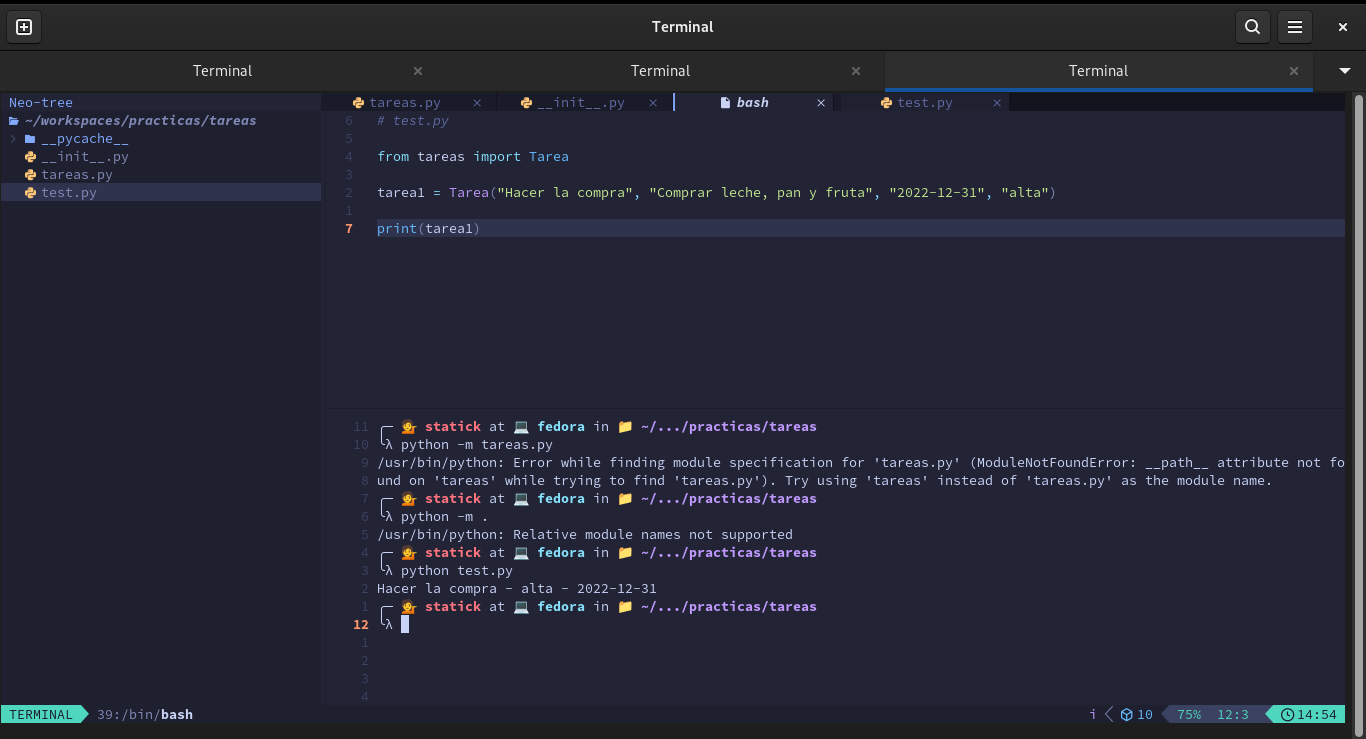
\includegraphics{unidades/Proyectos/images/proyecto_modulos.png}

}

\caption{Gestor de Tareas}

\end{figure}%

Una aplicación interactiva que permite organizar tus tareas de manera
eficiente, asignando prioridades y estableciendo fechas límite.

\section{Módulos del Proyecto}\label{muxf3dulos-del-proyecto}

\subsection{📋 Módulo de tareas}\label{muxf3dulo-de-tareas}

\begin{itemize}
\item
  Crear una nueva tarea con título, descripción, fecha límite y
  prioridad.
\item
  Marcar tareas como completadas ✅ o en progreso 🔄.
\item
  Organizar las tareas en orden de prioridad 🔥 o por fecha límite 📅.
\end{itemize}

\section{Funciones Clave}\label{funciones-clave}

\begin{itemize}
\tightlist
\item
  Prioriza tus tareas con un sistema de prioridades: baja, media y alta
  🔥.
\end{itemize}

\subsection{Desarrollo}\label{desarrollo}

Creamos la siguiente estructura de carpetas para organizar nuestro
proyecto:

\begin{Shaded}
\begin{Highlighting}[]
\NormalTok{proyecto\_modulos/}
\NormalTok{│}
\NormalTok{├── tareas/}
\NormalTok{│   ├── \_\_init\_\_.py}
\NormalTok{│   ├── tareas.py}
\NormalTok{│}
\end{Highlighting}
\end{Shaded}

En el archivo \textbf{tareas.py} definimos las clases y funciones
necesarias para gestionar las tareas.

\begin{Shaded}
\begin{Highlighting}[]
\CommentTok{\# tareas.py}

\KeywordTok{class}\NormalTok{ Tarea:}
    \KeywordTok{def} \FunctionTok{\_\_init\_\_}\NormalTok{(}\VariableTok{self}\NormalTok{, titulo, descripcion, fecha\_limite, prioridad):}
        \VariableTok{self}\NormalTok{.titulo }\OperatorTok{=}\NormalTok{ titulo}
        \VariableTok{self}\NormalTok{.descripcion }\OperatorTok{=}\NormalTok{ descripcion}
        \VariableTok{self}\NormalTok{.fecha\_limite }\OperatorTok{=}\NormalTok{ fecha\_limite}
        \VariableTok{self}\NormalTok{.prioridad }\OperatorTok{=}\NormalTok{ prioridad}
        \VariableTok{self}\NormalTok{.completada }\OperatorTok{=} \VariableTok{False}

    \KeywordTok{def}\NormalTok{ marcar\_completada(}\VariableTok{self}\NormalTok{):}
        \VariableTok{self}\NormalTok{.completada }\OperatorTok{=} \VariableTok{True}

    \KeywordTok{def}\NormalTok{ marcar\_en\_progreso(}\VariableTok{self}\NormalTok{):}
        \VariableTok{self}\NormalTok{.completada }\OperatorTok{=} \VariableTok{False}

    \KeywordTok{def} \FunctionTok{\_\_str\_\_}\NormalTok{(}\VariableTok{self}\NormalTok{):}
        \ControlFlowTok{return} \SpecialStringTok{f"}\SpecialCharTok{\{}\VariableTok{self}\SpecialCharTok{.}\NormalTok{titulo}\SpecialCharTok{\}}\SpecialStringTok{ {-} }\SpecialCharTok{\{}\VariableTok{self}\SpecialCharTok{.}\NormalTok{prioridad}\SpecialCharTok{\}}\SpecialStringTok{ {-} }\SpecialCharTok{\{}\VariableTok{self}\SpecialCharTok{.}\NormalTok{fecha\_limite}\SpecialCharTok{\}}\SpecialStringTok{"}
\end{Highlighting}
\end{Shaded}

En el archivo \textbf{\textbf{init}.py} definimos las funciones
principales para interactuar con las tareas.

\begin{Shaded}
\begin{Highlighting}[]
\CommentTok{\# \_\_init\_\_.py}

\ImportTok{from}\NormalTok{ tareas }\ImportTok{import}\NormalTok{ Tarea}

\KeywordTok{def}\NormalTok{ crear\_tarea(titulo, descripcion, fecha\_limite, prioridad):}
    \ControlFlowTok{return}\NormalTok{ Tarea(titulo, descripcion, fecha\_limite, prioridad)}

\KeywordTok{def}\NormalTok{ marcar\_completada(tarea):}
\NormalTok{    tarea.marcar\_completada()}

\KeywordTok{def}\NormalTok{ marcar\_en\_progreso(tarea):}
\NormalTok{    tarea.marcar\_en\_progreso()}
\end{Highlighting}
\end{Shaded}

Con esta estructura básica, podemos empezar a desarrollar la
funcionalidad de nuestro gestor de tareas. En los siguientes módulos,
ampliaremos las capacidades de nuestra aplicación y añadiremos nuevas
funcionalidades.

Para poder probar nuestro código, podemos crear un script de prueba en
la misma carpeta:

\begin{Shaded}
\begin{Highlighting}[]
\CommentTok{\# test.py}

\ImportTok{from}\NormalTok{ tareas }\ImportTok{import}\NormalTok{ Tarea}

\NormalTok{tarea1 }\OperatorTok{=}\NormalTok{ Tarea(}\StringTok{"Hacer la compra"}\NormalTok{, }\StringTok{"Comprar leche, pan y fruta"}\NormalTok{, }\StringTok{"2022{-}12{-}31"}\NormalTok{, }\StringTok{"alta"}\NormalTok{)}

\BuiltInTok{print}\NormalTok{(tarea1)}
\end{Highlighting}
\end{Shaded}

Al ejecutar el script de prueba, deberíamos ver la información de la
tarea creada.

\begin{Shaded}
\begin{Highlighting}[]
\ExtensionTok{$}\NormalTok{ python test.py}
\ExtensionTok{Hacer}\NormalTok{ la compra }\AttributeTok{{-}}\NormalTok{ alta }\AttributeTok{{-}}\NormalTok{ 2022{-}12{-}31}
\end{Highlighting}
\end{Shaded}

\chapter{Extra 🎁}\label{extra}

\begin{itemize}
\tightlist
\item
  Añadir la funcionalidad de editar y eliminar tareas.
\end{itemize}

\begin{Shaded}
\begin{Highlighting}[]
\KeywordTok{def}\NormalTok{ editar\_tarea(tarea, titulo}\OperatorTok{=}\VariableTok{None}\NormalTok{, descripcion}\OperatorTok{=}\VariableTok{None}\NormalTok{, fecha\_limite}\OperatorTok{=}\VariableTok{None}\NormalTok{, prioridad}\OperatorTok{=}\VariableTok{None}\NormalTok{):}
    \ControlFlowTok{if}\NormalTok{ titulo:}
\NormalTok{        tarea.titulo }\OperatorTok{=}\NormalTok{ titulo}
    \ControlFlowTok{if}\NormalTok{ descripcion:}
\NormalTok{        tarea.descripcion }\OperatorTok{=}\NormalTok{ descripcion}
    \ControlFlowTok{if}\NormalTok{ fecha\_limite:}
\NormalTok{        tarea.fecha\_limite }\OperatorTok{=}\NormalTok{ fecha\_limite}
    \ControlFlowTok{if}\NormalTok{ prioridad:}
\NormalTok{        tarea.prioridad }\OperatorTok{=}\NormalTok{ prioridad}
\end{Highlighting}
\end{Shaded}

\begin{itemize}
\tightlist
\item
  Implementar un sistema de notificaciones para recordar las fechas
  límite de las tareas.
\end{itemize}

\begin{Shaded}
\begin{Highlighting}[]
\ImportTok{import}\NormalTok{ datetime}

\KeywordTok{def}\NormalTok{ notificar\_tareas(tareas):}
\NormalTok{    hoy }\OperatorTok{=}\NormalTok{ datetime.date.today()}
    \ControlFlowTok{for}\NormalTok{ tarea }\KeywordTok{in}\NormalTok{ tareas:}
        \ControlFlowTok{if}\NormalTok{ tarea.fecha\_limite }\OperatorTok{==}\NormalTok{ hoy:}
            \BuiltInTok{print}\NormalTok{(}\SpecialStringTok{f"¡Recuerda! La tarea \textquotesingle{}}\SpecialCharTok{\{}\NormalTok{tarea}\SpecialCharTok{.}\NormalTok{titulo}\SpecialCharTok{\}}\SpecialStringTok{\textquotesingle{} vence hoy."}\NormalTok{)}
\end{Highlighting}
\end{Shaded}

\begin{itemize}
\tightlist
\item
  Crear una interfaz gráfica para una mejor experiencia de usuario.
\end{itemize}

\begin{Shaded}
\begin{Highlighting}[]
\ImportTok{import}\NormalTok{ tkinter }\ImportTok{as}\NormalTok{ tk}

\NormalTok{root }\OperatorTok{=}\NormalTok{ tk.Tk()}

\NormalTok{label }\OperatorTok{=}\NormalTok{ tk.Label(root, text}\OperatorTok{=}\StringTok{"Gestor de Tareas"}\NormalTok{)}
\NormalTok{label.pack()}

\NormalTok{root.mainloop()}
\end{Highlighting}
\end{Shaded}

\chapter{Conclusión}\label{conclusiuxf3n-3}

Con estos módulos básicos, hemos sentado las bases para desarrollar un
gestor de tareas con prioridades. A medida que añadamos más
funcionalidades y módulos, nuestra aplicación se volverá más completa y
útil para organizar nuestras tareas diarias.

\chapter{Reto 💡}\label{reto}

\begin{itemize}
\tightlist
\item
  Implementar un sistema de categorías para organizar las tareas por
  proyectos o áreas de interés.
\end{itemize}

\chapter{🛒 Simulador de Tienda
Online}\label{simulador-de-tienda-online}

\begin{figure}[H]

{\centering 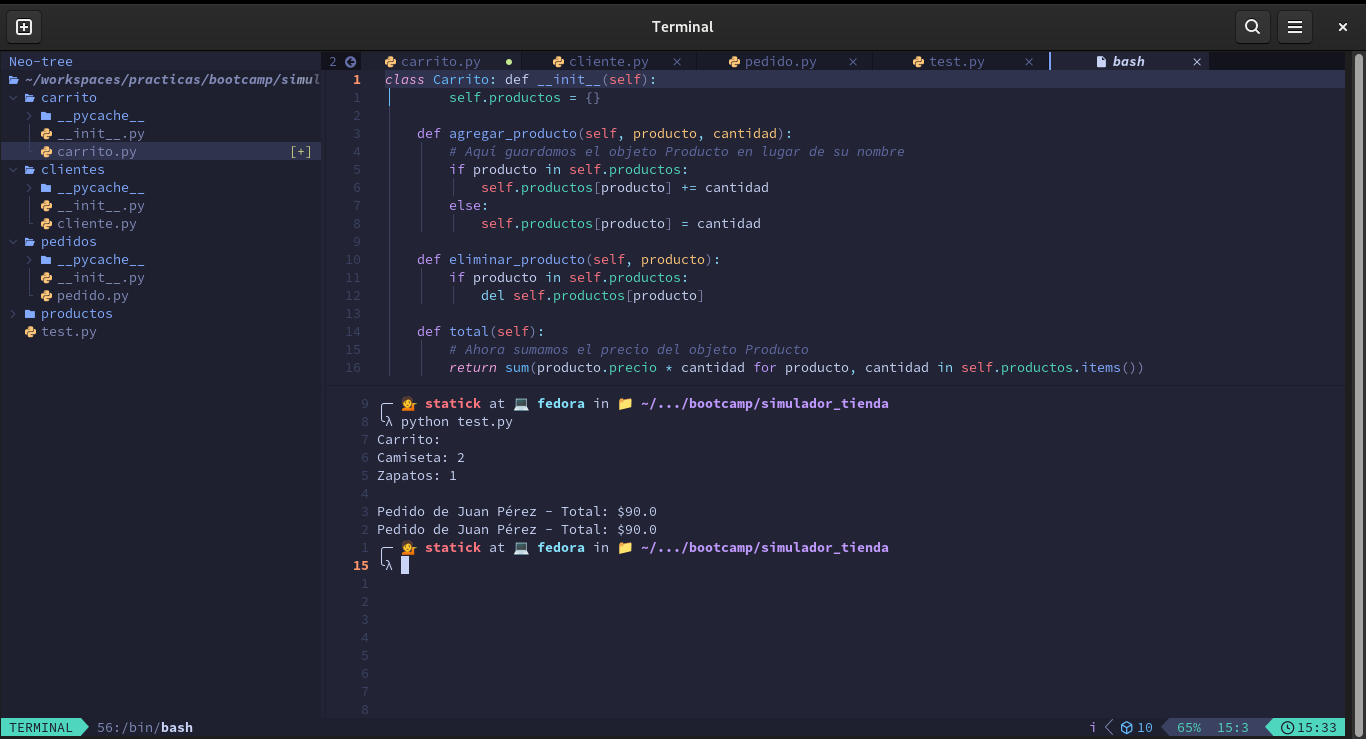
\includegraphics{unidades/Proyectos/images/tienda_online.png}

}

\caption{Tienda Online}

\end{figure}%

Un proyecto interactivo que simula una tienda en línea donde los
clientes pueden agregar productos al carrito, realizar pedidos,
gestionar inventarios y procesar pagos.

\section{Módulos del Proyecto}\label{muxf3dulos-del-proyecto-1}

\subsection{🛍️ Módulo de Productos}\label{muxf3dulo-de-productos}

\begin{enumerate}
\def\labelenumi{\arabic{enumi}.}
\tightlist
\item
  Definir productos con nombre, precio y cantidad en inventario.
\item
  Actualizar el inventario después de cada compra o cuando se agregan
  nuevos productos.
\end{enumerate}

\subsection{🛒 Módulo de Carrito}\label{muxf3dulo-de-carrito}

\begin{enumerate}
\def\labelenumi{\arabic{enumi}.}
\tightlist
\item
  Permite a los clientes agregar o quitar productos de su carrito.
\item
  Calcular el costo total de los productos en el carrito.
\end{enumerate}

\subsection{👤 Módulo de Cliente}\label{muxf3dulo-de-cliente}

\begin{enumerate}
\def\labelenumi{\arabic{enumi}.}
\tightlist
\item
  Gestionar la creación de nuevos clientes.
\item
  Mantener el historial de compras del cliente.
\end{enumerate}

\subsection{📦 Módulo de Pedido}\label{muxf3dulo-de-pedido}

\begin{enumerate}
\def\labelenumi{\arabic{enumi}.}
\tightlist
\item
  Procesar un pedido, verificar disponibilidad en inventario, y generar
  la factura.
\item
  Actualizar el inventario después de la compra.
\end{enumerate}

\chapter{Desarrollo}\label{desarrollo-1}

Creamos la siguiente estructura de carpetas para organizar nuestro
proyecto:

\begin{Shaded}
\begin{Highlighting}[]
\NormalTok{tienda\_online/}
\NormalTok{│}
\NormalTok{├── productos/}
\NormalTok{│   ├── \_\_init\_\_.py}
\NormalTok{│   ├── producto.py}
\NormalTok{│}
\NormalTok{├── clientes/}
\NormalTok{│   ├── \_\_init\_\_.py}
\NormalTok{│   ├── cliente.py}
\NormalTok{│}
\NormalTok{├── carrito/}
\NormalTok{│   ├── \_\_init\_\_.py}
\NormalTok{│   ├── carrito.py}
\NormalTok{│}
\NormalTok{├── pedidos/}
\NormalTok{│   ├── \_\_init\_\_.py}
\NormalTok{│   ├── pedido.py}
\end{Highlighting}
\end{Shaded}

Definimos las clases y funciones necesarias para gestionar la tienda en
línea.

\section{🛍️ Productos}\label{productos}

En el archivo \textbf{producto.py}, definimos la clase
\textbf{Producto}:

\begin{Shaded}
\begin{Highlighting}[]
\CommentTok{\# productos/producto.py}

\KeywordTok{class}\NormalTok{ Producto:}
    \KeywordTok{def} \FunctionTok{\_\_init\_\_}\NormalTok{(}\VariableTok{self}\NormalTok{, nombre, precio, inventario):}
        \VariableTok{self}\NormalTok{.nombre }\OperatorTok{=}\NormalTok{ nombre}
        \VariableTok{self}\NormalTok{.precio }\OperatorTok{=}\NormalTok{ precio}
        \VariableTok{self}\NormalTok{.inventario }\OperatorTok{=}\NormalTok{ inventario}

    \KeywordTok{def}\NormalTok{ actualizar\_inventario(}\VariableTok{self}\NormalTok{, cantidad):}
        \VariableTok{self}\NormalTok{.inventario }\OperatorTok{{-}=}\NormalTok{ cantidad}

    \KeywordTok{def} \FunctionTok{\_\_str\_\_}\NormalTok{(}\VariableTok{self}\NormalTok{):}
        \ControlFlowTok{return} \SpecialStringTok{f"}\SpecialCharTok{\{}\VariableTok{self}\SpecialCharTok{.}\NormalTok{nombre}\SpecialCharTok{\}}\SpecialStringTok{ {-} $}\SpecialCharTok{\{}\VariableTok{self}\SpecialCharTok{.}\NormalTok{precio}\SpecialCharTok{\}}\SpecialStringTok{ (Inventario: }\SpecialCharTok{\{}\VariableTok{self}\SpecialCharTok{.}\NormalTok{inventario}\SpecialCharTok{\}}\SpecialStringTok{)"}
\end{Highlighting}
\end{Shaded}

\section{🛒 Carrito}\label{carrito}

En el archivo \textbf{carrito.py}, definimos la clase Carrito:

\begin{Shaded}
\begin{Highlighting}[]
\CommentTok{\# carrito/carrito.py}

\KeywordTok{class}\NormalTok{ Carrito:}
    \KeywordTok{def} \FunctionTok{\_\_init\_\_}\NormalTok{(}\VariableTok{self}\NormalTok{):}
        \VariableTok{self}\NormalTok{.productos }\OperatorTok{=}\NormalTok{ \{\}}

    \KeywordTok{def}\NormalTok{ agregar\_producto(}\VariableTok{self}\NormalTok{, producto, cantidad):}
        \ControlFlowTok{if}\NormalTok{ producto.nombre }\KeywordTok{in} \VariableTok{self}\NormalTok{.productos:}
            \VariableTok{self}\NormalTok{.productos[producto.nombre] }\OperatorTok{+=}\NormalTok{ cantidad}
        \ControlFlowTok{else}\NormalTok{:}
            \VariableTok{self}\NormalTok{.productos[producto.nombre] }\OperatorTok{=}\NormalTok{ cantidad}

    \KeywordTok{def}\NormalTok{ eliminar\_producto(}\VariableTok{self}\NormalTok{, producto):}
        \ControlFlowTok{if}\NormalTok{ producto.nombre }\KeywordTok{in} \VariableTok{self}\NormalTok{.productos:}
            \KeywordTok{del} \VariableTok{self}\NormalTok{.productos[producto.nombre]}

    \KeywordTok{def}\NormalTok{ total(}\VariableTok{self}\NormalTok{):}
        \ControlFlowTok{return} \BuiltInTok{sum}\NormalTok{(producto.precio }\OperatorTok{*}\NormalTok{ cantidad }\ControlFlowTok{for}\NormalTok{ producto, cantidad }\KeywordTok{in} \VariableTok{self}\NormalTok{.productos.items())}

    \KeywordTok{def} \FunctionTok{\_\_str\_\_}\NormalTok{(}\VariableTok{self}\NormalTok{):}
\NormalTok{        carrito\_str }\OperatorTok{=} \StringTok{"Carrito:}\CharTok{\textbackslash{}n}\StringTok{"}
        \ControlFlowTok{for}\NormalTok{ producto, cantidad }\KeywordTok{in} \VariableTok{self}\NormalTok{.productos.items():}
\NormalTok{            carrito\_str }\OperatorTok{+=} \SpecialStringTok{f"}\SpecialCharTok{\{}\NormalTok{producto}\SpecialCharTok{\}}\SpecialStringTok{: }\SpecialCharTok{\{}\NormalTok{cantidad}\SpecialCharTok{\}}\CharTok{\textbackslash{}n}\SpecialStringTok{"}
        \ControlFlowTok{return}\NormalTok{ carrito\_str}
\end{Highlighting}
\end{Shaded}

\section{👤 Clientes}\label{clientes}

En el archivo \textbf{cliente.py}, definimos la clase \textbf{Cliente}:

\begin{Shaded}
\begin{Highlighting}[]
\CommentTok{\# clientes/cliente.py}

\KeywordTok{class}\NormalTok{ Cliente:}
    \KeywordTok{def} \FunctionTok{\_\_init\_\_}\NormalTok{(}\VariableTok{self}\NormalTok{, nombre, email):}
        \VariableTok{self}\NormalTok{.nombre }\OperatorTok{=}\NormalTok{ nombre}
        \VariableTok{self}\NormalTok{.email }\OperatorTok{=}\NormalTok{ email}
        \VariableTok{self}\NormalTok{.historial\_compras }\OperatorTok{=}\NormalTok{ []}

    \KeywordTok{def}\NormalTok{ agregar\_historial(}\VariableTok{self}\NormalTok{, pedido):}
        \VariableTok{self}\NormalTok{.historial\_compras.append(pedido)}

    \KeywordTok{def}\NormalTok{ ver\_historial(}\VariableTok{self}\NormalTok{):}
        \ControlFlowTok{if} \KeywordTok{not} \VariableTok{self}\NormalTok{.historial\_compras:}
            \ControlFlowTok{return} \StringTok{"No tienes compras aún."}
        \ControlFlowTok{return} \StringTok{"}\CharTok{\textbackslash{}n}\StringTok{"}\NormalTok{.join(}\BuiltInTok{str}\NormalTok{(pedido) }\ControlFlowTok{for}\NormalTok{ pedido }\KeywordTok{in} \VariableTok{self}\NormalTok{.historial\_compras)}

    \KeywordTok{def} \FunctionTok{\_\_str\_\_}\NormalTok{(}\VariableTok{self}\NormalTok{):}
        \ControlFlowTok{return} \SpecialStringTok{f"Cliente: }\SpecialCharTok{\{}\VariableTok{self}\SpecialCharTok{.}\NormalTok{nombre}\SpecialCharTok{\}}\SpecialStringTok{ (}\SpecialCharTok{\{}\VariableTok{self}\SpecialCharTok{.}\NormalTok{email}\SpecialCharTok{\}}\SpecialStringTok{)"}
\end{Highlighting}
\end{Shaded}

\section{📦 Pedidos}\label{pedidos}

En el archivo \textbf{pedido.py}, definimos la clase \textbf{Pedido}:

\begin{Shaded}
\begin{Highlighting}[]
\CommentTok{\# pedidos/pedido.py}

\KeywordTok{class}\NormalTok{ Pedido:}
    \KeywordTok{def} \FunctionTok{\_\_init\_\_}\NormalTok{(}\VariableTok{self}\NormalTok{, cliente, carrito):}
        \VariableTok{self}\NormalTok{.cliente }\OperatorTok{=}\NormalTok{ cliente}
        \VariableTok{self}\NormalTok{.carrito }\OperatorTok{=}\NormalTok{ carrito}
        \VariableTok{self}\NormalTok{.total }\OperatorTok{=}\NormalTok{ carrito.total()}

    \KeywordTok{def}\NormalTok{ procesar\_pedido(}\VariableTok{self}\NormalTok{):}
        \ControlFlowTok{for}\NormalTok{ producto, cantidad }\KeywordTok{in} \VariableTok{self}\NormalTok{.carrito.productos.items():}
\NormalTok{            producto.actualizar\_inventario(cantidad)}
        \VariableTok{self}\NormalTok{.cliente.agregar\_historial(}\VariableTok{self}\NormalTok{)}

    \KeywordTok{def} \FunctionTok{\_\_str\_\_}\NormalTok{(}\VariableTok{self}\NormalTok{):}
        \ControlFlowTok{return} \SpecialStringTok{f"Pedido de }\SpecialCharTok{\{}\VariableTok{self}\SpecialCharTok{.}\NormalTok{cliente}\SpecialCharTok{.}\NormalTok{nombre}\SpecialCharTok{\}}\SpecialStringTok{ {-} Total: $}\SpecialCharTok{\{}\VariableTok{self}\SpecialCharTok{.}\NormalTok{total}\SpecialCharTok{\}}\SpecialStringTok{"}
\end{Highlighting}
\end{Shaded}

\chapter{Prueba del Simulador de Tienda
Online}\label{prueba-del-simulador-de-tienda-online}

En un archivo de prueba test.py, puedes simular una compra en la tienda:

\begin{Shaded}
\begin{Highlighting}[]
\CommentTok{\# test.py}

\ImportTok{from}\NormalTok{ productos.producto }\ImportTok{import}\NormalTok{ Producto}
\ImportTok{from}\NormalTok{ carrito.carrito }\ImportTok{import}\NormalTok{ Carrito}
\ImportTok{from}\NormalTok{ clientes.cliente }\ImportTok{import}\NormalTok{ Cliente}
\ImportTok{from}\NormalTok{ pedidos.pedido }\ImportTok{import}\NormalTok{ Pedido}

\CommentTok{\# Crear productos}
\NormalTok{producto1 }\OperatorTok{=}\NormalTok{ Producto(}\StringTok{"Camiseta"}\NormalTok{, }\FloatTok{20.0}\NormalTok{, }\DecValTok{50}\NormalTok{)}
\NormalTok{producto2 }\OperatorTok{=}\NormalTok{ Producto(}\StringTok{"Zapatos"}\NormalTok{, }\FloatTok{50.0}\NormalTok{, }\DecValTok{20}\NormalTok{)}

\CommentTok{\# Crear un cliente}
\NormalTok{cliente }\OperatorTok{=}\NormalTok{ Cliente(}\StringTok{"Juan Pérez"}\NormalTok{, }\StringTok{"juan@example.com"}\NormalTok{)}

\CommentTok{\# Crear un carrito y agregar productos}
\NormalTok{carrito }\OperatorTok{=}\NormalTok{ Carrito()}
\NormalTok{carrito.agregar\_producto(producto1, }\DecValTok{2}\NormalTok{)}
\NormalTok{carrito.agregar\_producto(producto2, }\DecValTok{1}\NormalTok{)}

\BuiltInTok{print}\NormalTok{(carrito)  }\CommentTok{\# Ver contenido del carrito}

\CommentTok{\# Crear y procesar el pedido}
\NormalTok{pedido }\OperatorTok{=}\NormalTok{ Pedido(cliente, carrito)}
\NormalTok{pedido.procesar\_pedido()}

\BuiltInTok{print}\NormalTok{(pedido)  }\CommentTok{\# Ver detalles del pedido}
\BuiltInTok{print}\NormalTok{(cliente.ver\_historial())  }\CommentTok{\# Ver historial de compras}
\end{Highlighting}
\end{Shaded}

Al ejecutar el archivo test.py, verás el contenido del carrito, el
pedido procesado, y el historial de compras del cliente.

\chapter{Extra 🎁}\label{extra-1}

\begin{itemize}
\tightlist
\item
  Añadir la funcionalidad de eliminar productos del carrito:
\end{itemize}

\begin{Shaded}
\begin{Highlighting}[]
\KeywordTok{def}\NormalTok{ eliminar\_producto(}\VariableTok{self}\NormalTok{, producto):}
    \ControlFlowTok{if}\NormalTok{ producto }\KeywordTok{in} \VariableTok{self}\NormalTok{.productos:}
        \KeywordTok{del} \VariableTok{self}\NormalTok{.productos[producto]}
\end{Highlighting}
\end{Shaded}

\begin{itemize}
\tightlist
\item
  Añadir un sistema de descuento:
\end{itemize}

\begin{Shaded}
\begin{Highlighting}[]
\KeywordTok{def}\NormalTok{ aplicar\_descuento(}\VariableTok{self}\NormalTok{, porcentaje):}
    \VariableTok{self}\NormalTok{.total }\OperatorTok{{-}=} \VariableTok{self}\NormalTok{.total }\OperatorTok{*}\NormalTok{ (porcentaje }\OperatorTok{/} \DecValTok{100}\NormalTok{)}
\end{Highlighting}
\end{Shaded}

\begin{itemize}
\tightlist
\item
  Añadir una interfaz gráfica usando Tkinter:
\end{itemize}

\begin{Shaded}
\begin{Highlighting}[]
\ImportTok{import}\NormalTok{ tkinter }\ImportTok{as}\NormalTok{ tk}

\NormalTok{root }\OperatorTok{=}\NormalTok{ tk.Tk()}

\NormalTok{label }\OperatorTok{=}\NormalTok{ tk.Label(root, text}\OperatorTok{=}\StringTok{"¡Bienvenido a la Tienda Online!"}\NormalTok{)}
\NormalTok{label.pack()}

\NormalTok{root.mainloop()}
\end{Highlighting}
\end{Shaded}

\chapter{Conclusión}\label{conclusiuxf3n-4}

Con esta estructura básica de POO, hemos creado un simulador de tienda
online donde se gestionan productos, carritos, clientes y pedidos. A
medida que avances, puedes agregar más características como métodos de
pago, envío, y más opciones de interacción para los clientes.

¡Diviértete desarrollando y mejorando tu tienda online! 🚀



\end{document}
